%% RA-PatchTST: IEEE manuscript.
%% Default build: IEEE journal manuscript, single column, 12 pt (review/submission format).
%% Camera-ready two-column build:  pdflatex "\def\cameraready{1}%% RA-PatchTST: IEEE manuscript.
%% Default build: IEEE journal manuscript, single column, 12 pt (review/submission format).
%% Camera-ready two-column build:  pdflatex "\def\cameraready{1}%% RA-PatchTST: IEEE manuscript.
%% Default build: IEEE journal manuscript, single column, 12 pt (review/submission format).
%% Camera-ready two-column build:  pdflatex "\def\cameraready{1}%% RA-PatchTST: IEEE manuscript.
%% Default build: IEEE journal manuscript, single column, 12 pt (review/submission format).
%% Camera-ready two-column build:  pdflatex "\def\cameraready{1}\input{main}"
\ifdefined\cameraready
  \documentclass[journal]{IEEEtran}
\else
  \documentclass[journal,12pt,onecolumn]{IEEEtran}
\fi

\usepackage{cite}
\usepackage{amsmath,amssymb,amsfonts}
\usepackage{bm}
\usepackage{graphicx}
\usepackage{booktabs}
\usepackage{multirow}
\usepackage{array}
\usepackage{xcolor}
\usepackage{algorithm}
\usepackage{algpseudocode}
\usepackage{textcomp}
\usepackage{url}
\usepackage[hidelinks]{hyperref}
\graphicspath{{figures/}}
\interdisplaylinepenalty=2500

\ifdefined\cameraready
  \newcommand{\figwidth}{\textwidth}
  \newcommand{\colfig}{\columnwidth}
\else
  \newcommand{\figwidth}{0.98\textwidth}
  \newcommand{\colfig}{0.62\textwidth}
\fi

\newcommand{\X}{\mathbf{X}}
\newcommand{\Y}{\mathbf{Y}}
\newcommand{\R}{\mathbb{R}}
\DeclareMathOperator*{\argmin}{arg\,min}

\ifdefined\cameraready
  \newcommand{\colfit}[1]{\resizebox{\columnwidth}{!}{#1}}
\else
  \newcommand{\colfit}[1]{#1}
\fi
\makeatletter\newcommand{\tabin}[1]{\@@input tables/#1.tex }\makeatother
\hyphenation{Patch-TST RA-Patch-TST Trans-former}

\begin{document}

\title{RA-PatchTST: A Reliability-Aware Extension of PatchTST for Multivariate Time-Series Forecasting Under Corrupted Inputs}

\author{Jeevika~N,
        Jnanottam~G~Y,
        and~Mallegowda~M%
\thanks{The authors are with the Department of Computer Science and Engineering, Ramaiah Institute of Technology, MSR Nagar, MSRIT Post, Bengaluru 560054, India. This work was carried out as part of the course Artificial Intelligence and Machine Learning (24CS52), academic year 2026--27.}}

\markboth{RA-PatchTST: Reliability-Aware PatchTST Under Corrupted Inputs}%
{N \MakeLowercase{\textit{et al.}}: RA-PatchTST: Reliability-Aware PatchTST Under Corrupted Inputs}

\maketitle

\input{sections/00_abstract}
\input{sections/01_introduction}
\input{sections/02_literature}
\input{sections/03_problem}
\input{sections/04_methodology}
\input{sections/05_architecture}
\input{sections/06_implementation}
\input{sections/07_experiments}
\input{sections/08_results}
\input{sections/09_future}
\input{sections/10_conclusion}

\section*{Acknowledgment}
The authors thank the Department of Computer Science and Engineering, Ramaiah Institute of Technology, for computing access and guidance. The ETTh1 dataset was released by Zhou \textit{et al.}~\cite{informer} through the ETDataset repository~\cite{ettdata}. The PatchTST re-implementation follows the official code of Nie \textit{et al.}~\cite{patchtst_code}, and the data protocol follows the Time-Series-Library~\cite{tslib_code}.

\bibliographystyle{IEEEtran}
\bibliography{refs}

\appendices
\input{sections/11_appendix}

\end{document}
"
\ifdefined\cameraready
  \documentclass[journal]{IEEEtran}
\else
  \documentclass[journal,12pt,onecolumn]{IEEEtran}
\fi

\usepackage{cite}
\usepackage{amsmath,amssymb,amsfonts}
\usepackage{bm}
\usepackage{graphicx}
\usepackage{booktabs}
\usepackage{multirow}
\usepackage{array}
\usepackage{xcolor}
\usepackage{algorithm}
\usepackage{algpseudocode}
\usepackage{textcomp}
\usepackage{url}
\usepackage[hidelinks]{hyperref}
\graphicspath{{figures/}}
\interdisplaylinepenalty=2500

\ifdefined\cameraready
  \newcommand{\figwidth}{\textwidth}
  \newcommand{\colfig}{\columnwidth}
\else
  \newcommand{\figwidth}{0.98\textwidth}
  \newcommand{\colfig}{0.62\textwidth}
\fi

\newcommand{\X}{\mathbf{X}}
\newcommand{\Y}{\mathbf{Y}}
\newcommand{\R}{\mathbb{R}}
\DeclareMathOperator*{\argmin}{arg\,min}

\ifdefined\cameraready
  \newcommand{\colfit}[1]{\resizebox{\columnwidth}{!}{#1}}
\else
  \newcommand{\colfit}[1]{#1}
\fi
\makeatletter\newcommand{\tabin}[1]{\@@input tables/#1.tex }\makeatother
\hyphenation{Patch-TST RA-Patch-TST Trans-former}

\begin{document}

\title{RA-PatchTST: A Reliability-Aware Extension of PatchTST for Multivariate Time-Series Forecasting Under Corrupted Inputs}

\author{Jeevika~N,
        Jnanottam~G~Y,
        and~Mallegowda~M%
\thanks{The authors are with the Department of Computer Science and Engineering, Ramaiah Institute of Technology, MSR Nagar, MSRIT Post, Bengaluru 560054, India. This work was carried out as part of the course Artificial Intelligence and Machine Learning (24CS52), academic year 2026--27.}}

\markboth{RA-PatchTST: Reliability-Aware PatchTST Under Corrupted Inputs}%
{N \MakeLowercase{\textit{et al.}}: RA-PatchTST: Reliability-Aware PatchTST Under Corrupted Inputs}

\maketitle

\begin{abstract}
Patch-based Transformer forecasters such as PatchTST treat every input patch as equally trustworthy, yet sensor series routinely contain missing readings, measurement noise, spikes and shifts in level or scale. This paper presents RA-PatchTST, a reliability-aware extension of PatchTST that adds three small components to the original design: a patch reliability gate (a two-layer perceptron with 801 parameters that scores each patch between 0 and 1 and rescales its embedding), a shift-aware forecasting head that receives the mean and scale of each input window relative to the training statistics, which instance normalization would otherwise discard, and corruption-aware training, in which half of the training windows are corrupted on the fly while the loss is always computed against the clean future. The full model adds 993 parameters (1.2\%) to an 81,728-parameter backbone. We evaluate on the ETTh1 benchmark (17,420 hourly records, seven variables, chronological 12/4/4-month split, look-back 336, horizon 96) using five ablation variants, two random seeds and 22 fixed test conditions: clean data plus 21 seeded corruptions covering point-wise and 16-step missing values, Gaussian noise, spikes, segment-level shift and a mixed setting. Our PatchTST re-implementation reaches a clean test MSE of 0.379 against the published 0.375. RA-PatchTST lowers the mean MSE over the 21 corrupted conditions from 0.429 to 0.413 ($-3.7\%$), with the largest reductions under shift ($-11.0\%$), spikes ($-6.5\%$) and mixed damage ($-5.2\%$), at a cost of $+0.7\%$ on clean data and up to $+1.3\%$ under missing values. The ablation attributes about four fifths of the gain to corruption-aware training; the gate and the shift-aware head add a further $-0.8\%$, concentrated on shift. The gate assigns clearly lower weight to corrupted patches only for spikes. With one dataset, one horizon, two seeds and synthetic corruptions drawn from the training families, these results are preliminary evidence for the approach and do not establish general superiority.
\end{abstract}

\begin{IEEEkeywords}
Time-series forecasting, PatchTST, Transformer, robustness, distribution shift, data corruption, reliability gating, instance normalization, ablation study.
\end{IEEEkeywords}

\section{Introduction}
\label{sec:intro}

\IEEEPARstart{F}{orecasting} the next few days of a multivariate sensor series supports load planning in power networks, scheduling in industrial plants and maintenance of equipment such as power transformers. Deep forecasters for this task have changed quickly over the last five years. Informer~\cite{informer} and its successors Autoformer~\cite{autoformer} and FEDformer~\cite{fedformer} adapted the Transformer~\cite{vaswani} to long sequences. DLinear~\cite{dlinear} then showed that a single linear layer could match or beat these models on the standard long-term benchmarks, and PatchTST~\cite{patchtst} restored the lead of attention-based models by splitting each channel into short overlapping patches, treating each patch as a token and processing channels independently with shared weights. PatchTST is now a common baseline in forecasting studies and in benchmark libraries~\cite{tslib}.

These models are compared on clean benchmarks, while real sensor streams are noisy in several ways: readings go missing when a logger fails, analog channels pick up noise, transient faults produce isolated spikes, and recalibration or a change in operating regime moves a stretch of the series to a different level or scale~\cite{blazquez_anomaly,gama_drift}. In forecasting there are rarely labels that say which inputs are bad~\cite{seer}, so the model has to cope with corrupted inputs without being told where they are.

Two properties of PatchTST make it sensitive to such inputs. First, every patch enters the encoder with the same standing. The attention weights can in principle learn to ignore a damaged patch, but nothing in the architecture or the training signal encourages this. Second, PatchTST normalizes each input window by its own mean and standard deviation (the instance normalization of RevIN~\cite{revin}, without the affine part) and restores those statistics at the output. This helps under slow drift, but it also removes the information that would tell the model that a window sits at an unusual level relative to the training data. Recent analyses argue that window-local statistics cannot capture every kind of shift~\cite{fan,apt,revinrole}.

In our own baseline run, under the segment-level shift corruption described in Section~\ref{sec:exp}, the test MSE of a faithful PatchTST re-implementation on ETTh1 rises from 0.379 on clean inputs to 0.520 on average over four severity levels, and to 0.712 at the highest level. Spikes raise it to 0.458. Missing values and noise, by contrast, cost less than 0.015.

Existing remedies fall into three groups (Section~\ref{sec:lit}). Normalization-based methods such as RevIN~\cite{revin}, Dish-TS~\cite{dishts}, FAN~\cite{fan} and APT~\cite{apt} target distribution shift but do not weigh inputs by quality. Robustness-oriented frameworks such as SEER~\cite{seer}, RobustTSF~\cite{robusttsf} and TameR~\cite{tamer} address noisy or anomalous inputs, but either replace the forecaster with a new architecture, focus on one type of damage, or act only at training time~\cite{tps}. Expert-based and test-time methods such as TFPS~\cite{tfps} and SOLID~\cite{solid} add parameters or per-sample fine-tuning. None of the studies we surveyed offers a small plug-in for PatchTST that scores the reliability of each patch and gives the head a global view of shift within a single forward pass; we make no claim about work outside that set.

This paper studies whether such a plug-in helps, and by how much. We make four contributions.
\begin{enumerate}
\item A reproducible corruption benchmark on ETTh1 with 22 fixed test conditions (clean plus five corruption families at four severity levels and one mixed setting), in which every model sees identical corrupted inputs.
\item RA-PatchTST, which adds to PatchTST a patch reliability gate, two shift features appended to the forecasting head, and corruption-aware training, for 993 extra parameters in total.
\item An ablation over five variants (A0 to A4) and two seeds that separates the contribution of training on corrupted data from that of each architectural component, together with a direct check of whether the gate down-weights corrupted patches.
\item A browser-based live laboratory in which the original and the proposed model run side by side on real ETTh1 test windows that the user can damage interactively.
\end{enumerate}

RA-PatchTST reduces the average corrupted-input MSE by 3.7\% and the shift error by 11.0\%, but most of this gain comes from corruption-aware training, the gate is a weak detector except for spikes, and the model is slightly worse than PatchTST on clean data and under missing values. The PatchTST backbone is a re-implementation of the published design~\cite{patchtst,patchtst_code}; the research contribution lies in the gate, the shift features, their combination with corruption-aware training, and the ablation that measures what each part adds.

The rest of the paper is organized as follows. Section~\ref{sec:lit} reviews related work. Section~\ref{sec:problem} states the problem formally. Section~\ref{sec:method} develops the method, Section~\ref{sec:arch} describes the system architecture and Section~\ref{sec:impl} the implementation. Section~\ref{sec:exp} gives the experimental protocol and Section~\ref{sec:results} the results and their discussion. Sections~\ref{sec:future} and~\ref{sec:conclusion} outline future work and conclude.

\section{Literature Review}
\label{sec:lit}

We carried out a focused narrative review. We searched arXiv, the proceedings of ICLR, ICML, NeurIPS, AAAI and KDD, and the Google Scholar and GitHub pages of the papers found, using the terms \emph{PatchTST}, \emph{patch-based forecasting}, \emph{robust time series forecasting}, \emph{distribution shift}, \emph{instance normalization}, \emph{missing values} and \emph{anomalies}, for the period 2021 to 2026. A study was kept if it builds on or compares with patch-based Transformers, if it addresses corrupted inputs or distribution shift in forecasting, or if it defines the benchmark protocol. Several 2026 entries were preprints at the time of writing. Because the papers use different datasets, horizons and protocols, we do not compare their numbers with ours.

\subsection{From Sequence Transformers to Patch Tokens}

The Transformer~\cite{vaswani} replaced recurrence with self-attention, and Informer~\cite{informer} was among the first to adapt it to long-sequence time-series forecasting, introducing ProbSparse attention and, with it, the ETT datasets that remain a standard benchmark. Autoformer~\cite{autoformer} built series decomposition into the network and replaced point-wise attention with an auto-correlation mechanism, and FEDformer~\cite{fedformer} moved attention into the frequency domain. Zeng \textit{et al.}~\cite{dlinear} then questioned the whole line of work: one-layer linear models with a trend-seasonal split (DLinear) outperformed these Transformers on nine benchmarks, suggesting that point-wise tokens carry too little semantic content for attention to exploit.

PatchTST~\cite{patchtst} answered this by grouping consecutive time steps into patches, in the same spirit as the image patches of the Vision Transformer~\cite{vit}. A look-back of 336 steps cut into patches of 16 with stride 8 gives 42 tokens per channel, which shortens the attention span by a factor of about eight and gives each token local shape information. PatchTST also processes each channel independently with shared weights, and normalizes each input window with its own statistics. The official implementation~\cite{patchtst_code} uses BatchNorm inside the encoder~\cite{batchnorm}, GELU activations~\cite{gelu} and residual attention scores in the style of RealFormer~\cite{realformer}. On ETTh1 with look-back 336 and horizon 96, the supervised PatchTST/42 reports MSE 0.375 and MAE 0.399~\cite{patchtst}.

Later models moved in several directions. TimesNet~\cite{timesnet} reshapes a series into two-dimensional period-by-phase tensors. iTransformer~\cite{itransformer} inverts the token axis and attends across variables instead of time. TimeMixer~\cite{timemixer} mixes seasonal and trend components across scales with MLPs, and xPatch~\cite{xpatch} combines patching with exponential seasonal-trend decomposition in a dual-stream CNN and MLP network. Chronos~\cite{chronos} takes the foundation-model route, scaling and quantizing values into tokens and training a language-model architecture on a large corpus for zero-shot use. The Time-Series-Library survey and benchmark~\cite{tslib,tslib_code} fixes a common protocol for these models, which we follow.

\subsection{Normalization and Distribution Shift}

A forecaster trained on one period and applied to the next faces distribution shift, a problem studied in machine learning under the names dataset shift~\cite{datasetshift} and concept drift~\cite{gama_drift}. RevIN~\cite{revin} handles it by normalizing each input window and restoring its statistics at the output, with optional learnable affine parameters. Non-stationary Transformers~\cite{nstransformer} combine such series stationarization with a de-stationary attention that reinjects the removed statistics into the attention scores, which is the closest prior idea to our shift-aware head. Dish-TS~\cite{dishts} separates the shift within the look-back window from the shift between look-back and horizon. FAN~\cite{fan} argues that mean and variance do not describe non-stationarity in the frequency domain and removes the dominant Fourier components instead. APT~\cite{apt} adds affine prototypes indexed by timestamp because, in its authors' analysis, local mean and variance miss global shift. An analysis of RevIN using PatchTST~\cite{revinrole} finds that some of its parts are redundant or even harmful, and that it does not cover all forms of shift. TS\_Adam~\cite{tsadam} changes the optimizer to cope with drift during training.

Two methods react to shift more actively. TFPS~\cite{tfps} identifies patch-level distribution shift and routes patches to pattern-specific experts in the time and frequency domains. SOLID~\cite{solid} detects context-driven shift and fine-tunes the prediction layer for each test sample on similar training samples, which adds computation at test time just as TFPS adds experts.

\subsection{Robustness to Corrupted Inputs}

Missing values are usually handled by imputation before forecasting, with recurrent models such as BRITS~\cite{brits} or self-attention models such as SAITS~\cite{saits}; anomalies are usually handled by detection~\cite{blazquez_anomaly}. Both add a separate model with its own training and error. Several recent works instead make the forecaster itself tolerant to corruption. RobustTSF~\cite{robusttsf} analyzes forecasting when the training data contain anomalies and proposes a robust training procedure. TameR~\cite{tamer} uses global context to reduce the bias of forecasters toward recent, possibly corrupted, observations and reports gains under noise, missing values and anomalies. SEER~\cite{seer} is the closest work to ours: a Transformer framework with a channel-adaptive module and a learnable patch replacement module that filters low-quality patches, tested under missing values, shifts, anomalies and noise. SEER is a full framework, whereas we ask how much of the benefit a far smaller addition to an unchanged PatchTST can deliver. Temporal Patch Shuffle~\cite{tps} augments training data by shuffling patches and improves the robustness of several model families, PatchTST included, but at test time every patch is still trusted equally.

Our evaluation design borrows from computer vision, where Hendrycks and Dietterich~\cite{hendrycks_corrupt} defined a benchmark of common corruptions at graded severities applied to the test set only. A study of Autoformer, Informer and PatchTST on synthetic signals~\cite{synthbench} similarly compares architectures under controlled noise. Training on corrupted copies of the input is a form of data augmentation, which the survey of Wen \textit{et al.}~\cite{tsaug_survey} reviews for time series.

\subsection{Gating as a Soft Selection Mechanism}

Multiplicative gates with sigmoid outputs are a standard way to let a network decide how much of a signal to pass. LSTM gates~\cite{lstm} control the flow of memory, gated linear units~\cite{glu} modulate convolutional features, and squeeze-and-excitation blocks~\cite{senet} rescale feature channels using a small bottleneck MLP over pooled statistics. Our reliability gate follows the last pattern most closely: a small MLP reads summary statistics of each patch and outputs a scale factor applied to that patch's embedding.

\subsection{Summary and Research Gap}

Table~\ref{tab:lit} summarizes the studies most relevant to this work. Shift-oriented methods change normalization or add experts, but none of them weighs inputs by their quality. The robustness-oriented methods do address corrupted inputs, each in its own way: SEER and TameR with new architectures, RobustTSF with a focus on anomalies, and TPS through augmentation at training time only. The accuracy-oriented models address neither problem. None of them tests how far a few hundred parameters added to an unchanged PatchTST can go, or which of the possible additions helps; Sections~\ref{sec:method} and~\ref{sec:results} take up both questions.

\begin{table*}[!t]
\centering
\caption{Studies Most Relevant to This Work and the Gap Each Leaves Open}
\label{tab:lit}
\footnotesize
\renewcommand{\arraystretch}{1.15}
\begin{tabular}{@{}p{0.17\textwidth}p{0.36\textwidth}p{0.40\textwidth}@{}}
\toprule
Study (venue, year) & Approach & Relevance and limitation for this work \\
\midrule
SEER~\cite{seer} (ICML 2026) & Channel-adaptive module and learnable patch replacement that filters low-quality patches & Closest aim; a full new framework rather than a small add-on to PatchTST \\
APT~\cite{apt} (AAAI 2026) & Affine prototypes indexed by timestamp for shift & Shift only; motivates giving the model global statistics \\
TameR~\cite{tamer} (ICML 2026) & Global context against recent-data bias & Robust to noise, missing values and anomalies; no per-patch reliability score \\
TPS~\cite{tps} (preprint, 2026) & Patch shuffling as training augmentation & Training time only; all patches trusted equally at test time \\
RevIN analysis~\cite{revinrole} (preprint, 2026) & Ablation of RevIN components with PatchTST & Analysis only; supports adding a global view of shift \\
TS\_Adam~\cite{tsadam} (Neurocomputing, 2026) & Optimizer modified for drift & Cannot distinguish reliable from unreliable inputs \\
xPatch~\cite{xpatch} (AAAI 2025) & Dual-stream patching with exponential decomposition & Accuracy-oriented; no input-quality mechanism \\
TFPS~\cite{tfps} (NeurIPS 2025) & Pattern-specific experts for patch-level shift & More parameters; targets shift rather than noise or missing data \\
FAN~\cite{fan} (NeurIPS 2024) & Frequency adaptive normalization & Shift only; does not weigh patches by quality \\
RobustTSF~\cite{robusttsf} (ICLR 2024) & Robust training with anomalous data & Anomalies only; not patch-based \\
SOLID~\cite{solid} (KDD 2024) & Detect context-driven shift, fine-tune per sample & Costly at test time; our gate needs one forward pass \\
iTransformer~\cite{itransformer}, TimeMixer~\cite{timemixer} (ICLR 2024) & Variate tokens; multiscale MLP mixing & Accuracy-oriented baselines \\
Chronos~\cite{chronos} (TMLR 2024) & Pretrained tokenized forecaster & Large pretrained model; not a lightweight fix \\
DLinear~\cite{dlinear} (AAAI 2023) & Linear model with decomposition & Strong simple baseline; no robustness mechanism \\
PatchTST~\cite{patchtst} (ICLR 2023) & Patching, channel independence, instance norm. & Base model; equal trust in all patches, window-local statistics only \\
RevIN~\cite{revin} (ICLR 2022) & Reversible instance normalization & Uses only the window's own mean and variance \\
\bottomrule
\end{tabular}
\end{table*}

\section{Problem Statement}
\label{sec:problem}

\subsection{Forecasting Setting}

Let $\{\mathbf{s}_t\}_{t=1}^{T_{\mathrm{tot}}}$, $\mathbf{s}_t\in\R^{C}$, be a multivariate series with $C$ channels sampled at regular intervals. At time $t$ a forecaster receives the look-back window $\X=[\mathbf{s}_{t-L+1},\dots,\mathbf{s}_t]^{\top}\in\R^{L\times C}$ and predicts the next $H$ steps $\Y=[\mathbf{s}_{t+1},\dots,\mathbf{s}_{t+H}]^{\top}\in\R^{H\times C}$. In this work $C=7$, $L=336$ and $H=96$, so the model reads two weeks of hourly data and forecasts the next four days. A forecaster $f_\theta$ is trained by minimizing the mean squared error
\begin{equation}
\mathcal{L}(\theta)=\mathbb{E}_{(\X,\Y)}\Big[\tfrac{1}{HC}\big\lVert f_\theta(\X)-\Y\big\rVert_F^2\Big].
\label{eq:mse}
\end{equation}

\subsection{Corrupted Inputs}

In deployment the model may receive a corrupted window $\tilde{\X}=\mathcal{C}(\X;\,\kappa,\ell,\xi)$, where $\mathcal{C}$ is a corruption operator of type $\kappa$ (missing values, noise, spike, shift or a mixture), severity $\ell$, and random draw $\xi$. The location of the damage is unknown to the model; we write $\mathbf{M}\in\{0,1\}^{L\times C}$ for the mask of altered positions, which is used only for analysis. The forecast target is never corrupted: the goal is to predict the true future $\Y$ from damaged evidence $\tilde{\X}$. Section~\ref{sec:method-corrupt} defines $\mathcal{C}$ precisely.

\subsection{Problem Definition}

Given a PatchTST forecaster, the problem is to keep the forecast error low when the input is corrupted, with three constraints that make the result usable as a plug-in:
\begin{enumerate}
\item the error on clean inputs should not rise by more than 2\%;
\item the parameter count should not rise by more than 5\%;
\item the model must run in a single forward pass, without a separate imputation or detection model and without test-time adaptation.
\end{enumerate}

\subsection{Research Questions and Hypotheses}

\textit{RQ1:} How much accuracy does a faithful PatchTST lose under controlled input corruption, and which corruption types hurt most?

\textit{RQ2:} Can a reliability gate, a shift-aware head and corruption-aware training reduce that loss, and how much does each contribute?

We test two hypotheses separately.
\begin{itemize}
\item \textbf{H1.} Together, the three components lower the test MSE of PatchTST averaged over the corrupted conditions, while the clean-data MSE changes only slightly.
\item \textbf{H2.} The gate learns to assign lower weight to corrupted patches than to clean patches.
\end{itemize}

\subsection{Objectives and Success Criteria}

Table~\ref{tab:objectives} lists the objectives and how each is measured. The numerical thresholds are practical targets we set for a lightweight add-on, not standards from the literature. The original plan to cover four datasets (ETTh1, ETTm1, Weather, Electricity) and four horizons was reduced to ETTh1 at horizon 96 because all training ran on CPUs; Section~\ref{sec:limitations} returns to this.

\begin{table}[!t]
\centering
\caption{Objectives and Success Criteria}
\label{tab:objectives}
\footnotesize
\renewcommand{\arraystretch}{1.15}
\colfit{%
\begin{tabular}{@{}p{0.06\linewidth}p{0.42\linewidth}p{0.44\linewidth}@{}}
\toprule
ID & Objective & Measure and target \\
\midrule
O1 & Re-implement PatchTST and reproduce its clean ETTh1 result & Test MSE within 2\% of the published 0.375 \\
O2 & Build a seeded corruption benchmark & 22 conditions; identical inputs for all models \\
O3 & Design RA-PatchTST & Parameter increase below 5\% \\
O4 & Compare A0 with variants A1 to A4 & Mean corrupted MSE lower than A0 in every seed; clean MSE increase below 2\% \\
O5 & Check what the gate learns & Mean gate weight on corrupted vs.\ clean patches \\
O6 & Build an interactive demonstration & Browser port agrees with PyTorch within $10^{-5}$ \\
\bottomrule
\end{tabular}}
\end{table}

\section{Proposed Methodology}
\label{sec:method}

RA-PatchTST keeps the PatchTST backbone unchanged and adds three components (Fig.~\ref{fig:arch}). This section first describes data preparation and the backbone, then each addition, the corruption model used for training and testing, and the training objective.

\begin{figure*}[!t]
\centering
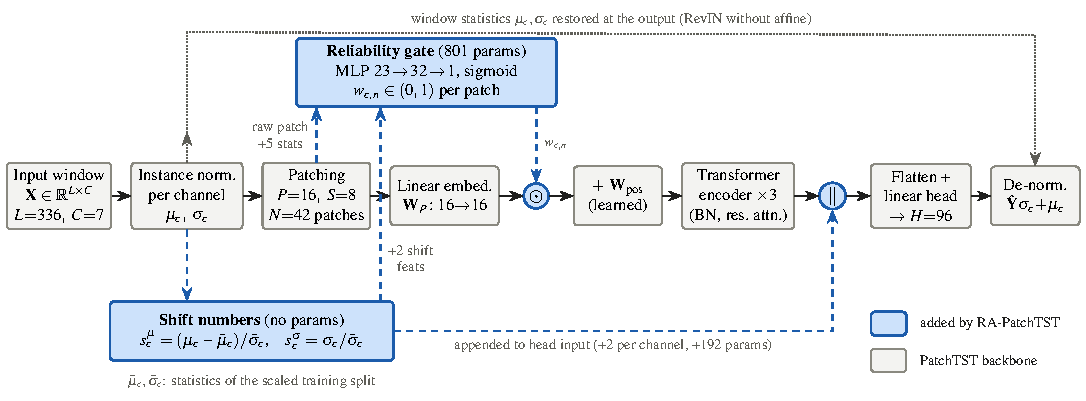
\includegraphics[width=\figwidth]{fig_architecture.pdf}
\caption{RA-PatchTST architecture. Grey blocks are the PatchTST backbone; blue blocks are the components added in this work. The reliability gate scores every patch and rescales its embedding before the position encoding is added; the two shift numbers are computed from the window statistics that instance normalization removes and are appended to the input of the linear head. Corruption-aware training (Fig.~\ref{fig:cat}) changes only the data fed to this network.}
\label{fig:arch}
\end{figure*}

\subsection{Data Preparation}
\label{sec:method-data}

The series is split chronologically into training, validation and test segments (Section~\ref{sec:exp}). A per-channel z-score scaler is fitted on the training segment only and applied to all three,
\begin{equation}
\begin{gathered}
\bar{s}_{t,c}=\frac{s_{t,c}-m_c}{d_c},\qquad m_c=\frac{1}{T_{\mathrm{tr}}}\sum_{t\le T_{\mathrm{tr}}}s_{t,c},\\
d_c^2=\frac{1}{T_{\mathrm{tr}}}\sum_{t\le T_{\mathrm{tr}}}(s_{t,c}-m_c)^2,
\end{gathered}
\label{eq:scale}
\end{equation}
so that no validation or test statistics leak into training. Windows of length $L+H$ are then cut with stride 1. Validation and test windows start $L$ steps before their segment so that the first forecast target lies exactly on the segment border, as in the Time-Series-Library protocol~\cite{tslib_code}. We also store the per-channel mean $\bar{\mu}_c$ and standard deviation $\bar{\sigma}_c$ of the \emph{scaled} training segment, which the shift features use. By construction $\bar{\mu}_c=0$ and $\bar{\sigma}_c=1$ up to rounding; the code keeps them explicit so that the same model can be used with other scalers.

\subsection{PatchTST Backbone}
\label{sec:method-backbone}

\subsubsection{Instance normalization}
For each window and channel the model computes
\begin{equation}
\begin{gathered}
\mu_c=\frac{1}{L}\sum_{i=1}^{L}x_{i,c},\qquad \sigma_c=\sqrt{\frac{1}{L}\sum_{i=1}^{L}(x_{i,c}-\mu_c)^2+\varepsilon},\\
x^{N}_{i,c}=\frac{x_{i,c}-\mu_c}{\sigma_c},
\end{gathered}
\label{eq:revin}
\end{equation}
with $\varepsilon=10^{-5}$. The statistics are treated as constants during back-propagation. This is RevIN~\cite{revin} without the learnable affine parameters, matching the configuration of the official PatchTST script for ETTh1.

\subsubsection{Patching}
Each normalized channel $\mathbf{x}^{N}_{c}\in\R^{L}$ is padded at the end with $S$ copies of its last value and unfolded into overlapping patches of length $P$ with stride $S$ (Fig.~\ref{fig:patching}):
\begin{equation}
\begin{gathered}
\mathbf{p}_{c,n}=\big[x^{N}_{nS+1,c},\dots,x^{N}_{nS+P,c}\big]^{\top}\in\R^{P},\\
n=0,\dots,N-1,\qquad N=\Big\lfloor\frac{L-P}{S}\Big\rfloor+2.
\end{gathered}
\label{eq:patch}
\end{equation}
With $L=336$, $P=16$ and $S=8$ this gives $N=42$ patches per channel, hence the name PatchTST/42.

\begin{figure}[!t]
\centering
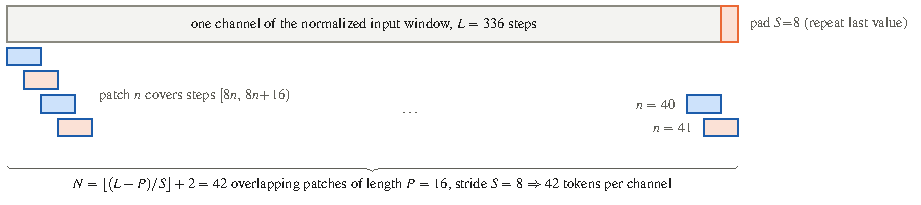
\includegraphics[width=\colfig]{fig_patching.pdf}
\caption{Patching of one channel. End padding with $S$ repeated values adds one patch, giving $N=42$ tokens for $L=336$, $P=16$, $S=8$.}
\label{fig:patching}
\end{figure}

\subsubsection{Embedding and encoder}
Each patch is mapped to a $D$-dimensional token by a shared linear layer, and a learnable position encoding $\mathbf{W}_{\mathrm{pos}}\in\R^{N\times D}$ is added:
\begin{equation}
\mathbf{e}_{c,n}=\mathbf{W}_P\,\mathbf{p}_{c,n}+\mathbf{b}_P,\qquad \mathbf{u}^{(0)}_{c,n}=\mathbf{e}_{c,n}+\mathbf{W}_{\mathrm{pos},n}.
\label{eq:embed}
\end{equation}
Channels are processed independently: the batch of $B$ windows becomes $B\cdot C$ sequences of $N$ tokens. Each of the three encoder layers applies multi-head self-attention with residual attention scores~\cite{realformer}, followed by a position-wise feed-forward network, each wrapped in a residual connection and BatchNorm~\cite{batchnorm}. For head $h$ in layer $l$,
\begin{equation}
\begin{gathered}
\mathbf{A}^{(l)}_h=\frac{\mathbf{Q}^{(l)}_h{\mathbf{K}^{(l)}_h}^{\top}}{\sqrt{d_k}}+\mathbf{A}^{(l-1)}_h,\\
\mathrm{head}^{(l)}_h=\mathrm{softmax}\big(\mathbf{A}^{(l)}_h\big)\,\mathbf{V}^{(l)}_h,
\end{gathered}
\label{eq:attn}
\end{equation}
where $\mathbf{A}^{(0)}_h=\mathbf{0}$ and $d_k=D/n_h$. The layer output is
\begin{align}
\mathbf{z}^{(l)}&=\mathrm{BN}\big(\mathbf{u}^{(l-1)}+\mathrm{Drop}(\mathrm{MHA}(\mathbf{u}^{(l-1)})\mathbf{W}_O)\big),\label{eq:layer1}\\
\mathbf{u}^{(l)}&=\mathrm{BN}\big(\mathbf{z}^{(l)}+\mathrm{Drop}(\mathbf{W}_2\,\mathrm{GELU}(\mathbf{W}_1\mathbf{z}^{(l)}))\big),\label{eq:layer2}
\end{align}
with GELU activation~\cite{gelu} and dropout~\cite{dropout}. We use $D=16$, $n_h=4$, a feed-forward width of 128 and dropout 0.3, the official settings for ETTh1.

\subsubsection{Head and de-normalization}
The $N$ output tokens of each channel are flattened into $\mathbf{h}_c\in\R^{ND}$ ($ND=672$), mapped to the horizon by a linear head, and the window statistics are restored:
\begin{equation}
\hat{\mathbf{y}}^{N}_c=\mathbf{W}_H\mathbf{h}_c+\mathbf{b}_H\in\R^{H},\qquad \hat{\mathbf{y}}_c=\sigma_c\,\hat{\mathbf{y}}^{N}_c+\mu_c.
\label{eq:head}
\end{equation}

\subsection{Patch Reliability Gate}
\label{sec:method-gate}

The gate is a small MLP that assigns every patch a weight $w_{c,n}\in(0,1)$ (Fig.~\ref{fig:gate}). Its input concatenates the 16 normalized values of the patch with seven summary features:
\begin{equation}
\begin{split}
\mathbf{g}_{c,n}=\mathrm{clip}_{[-10,10]}\Big(\big[&\mathbf{p}_{c,n};\ \bar{p}_{c,n};\ \varsigma_{c,n};\ j_{c,n};\\
&z_{c,n};\ a_{c,n};\ s^{\mu}_c;\ s^{\sigma}_c\big]\Big)\in\R^{23}.
\end{split}
\label{eq:gatein}
\end{equation}
Here $\bar{p}_{c,n}$ and $\varsigma_{c,n}$ are the mean and standard deviation of the patch, and $a_{c,n}=\max_k|p_{c,n,k}|$ is its largest absolute value. The jump feature compares a patch's mean with the average of its neighbours,
\begin{equation}
j_{c,n}=\Big|\bar{p}_{c,n}-\tfrac12\big(\bar{p}_{c,n-1}+\bar{p}_{c,n+1}\big)\Big|,
\label{eq:jump}
\end{equation}
with the first and last patch mean repeated at the borders. The zero share $z_{c,n}$ is the fraction of values in the corresponding patch of the \emph{un-normalized} (scaled) input that are exactly zero; it was designed to expose missing values, which the corruption model fills with the training mean, i.e., zero after scaling. The last two entries are the window-level shift features defined in~\eqref{eq:shift} below, broadcast to every patch of the channel. The gate is
\begin{equation}
w_{c,n}=\mathrm{sigmoid}\Big(\mathbf{v}_2^{\top}\,\mathrm{ReLU}\big(\mathbf{V}_1\mathbf{g}_{c,n}+\mathbf{c}_1\big)+c_2\Big),
\label{eq:gate}
\end{equation}
with $\mathbf{V}_1\in\R^{32\times23}$, $\mathbf{c}_1,\mathbf{v}_2\in\R^{32}$ and $c_2\in\R$. The weight rescales the patch embedding before the position encoding is added, replacing~\eqref{eq:embed} by
\begin{equation}
\mathbf{u}^{(0)}_{c,n}=w_{c,n}\big(\mathbf{W}_P\,\mathbf{p}_{c,n}+\mathbf{b}_P\big)+\mathbf{W}_{\mathrm{pos},n}.
\label{eq:gated}
\end{equation}
Applying the gate before the position encoding means that a fully distrusted patch still occupies its position in the sequence but carries no content. The output bias is initialized to $c_2=4$, so that $w\approx\mathrm{sigmoid}(4)\approx0.982$ at the start of training and the model initially behaves like PatchTST. The gate has $23\cdot32+32+32+1=801$ parameters. No supervision tells the gate which patches are corrupted; it is trained only through the forecasting loss. The code also supports an optional penalty $\lambda(1-\bar{w})$ that discourages uniformly low weights, but it was not used ($\lambda=0$) in any reported run.

\begin{figure}[!t]
\centering
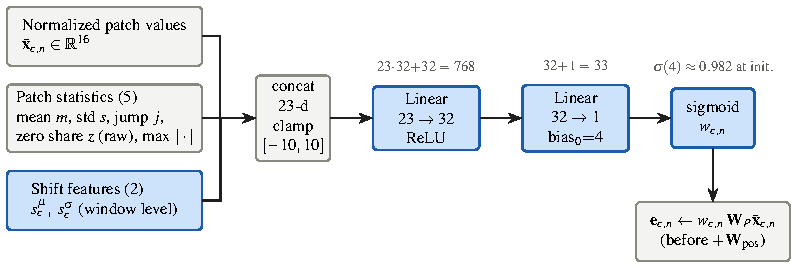
\includegraphics[width=\linewidth]{fig_gate.pdf}
\caption{Reliability gate. Each patch is scored from its 16 normalized values, five patch statistics and the two shift features of its channel. The score multiplies the patch embedding.}
\label{fig:gate}
\end{figure}

\subsection{Shift-Aware Head}
\label{sec:method-shift}

Instance normalization~\eqref{eq:revin} makes the encoder blind to where a window sits relative to the data the model was trained on: a window whose level has moved by two standard deviations looks the same after normalization as an ordinary one. The window statistics are added back at the output~\eqref{eq:head}, but only as an affine correction, so the shape of the forecast cannot depend on them. We compute two shift numbers per channel,
\begin{equation}
s^{\mu}_c=\frac{\mu_c-\bar{\mu}_c}{\bar{\sigma}_c},\qquad s^{\sigma}_c=\frac{\sigma_c}{\bar{\sigma}_c},
\label{eq:shift}
\end{equation}
and append them to the flattened encoder output before the head:
\begin{equation}
\hat{\mathbf{y}}^{N}_c=\mathbf{W}'_H\big[\mathbf{h}_c;\ s^{\mu}_c;\ s^{\sigma}_c\big]+\mathbf{b}_H,\qquad \mathbf{W}'_H\in\R^{H\times(ND+2)}.
\label{eq:shifthead}
\end{equation}
This adds $2H=192$ parameters. The idea is related to the de-stationary attention of Non-stationary Transformers~\cite{nstransformer}, which also reinjects removed statistics, but here they enter only the linear head. The same two numbers feed the gate.

\subsection{Corruption Model}
\label{sec:method-corrupt}

All corruptions act on scaled input windows, so a unit of one corresponds to one training standard deviation. Let $\mathbf{M}$ denote the mask of altered positions, $\odot$ the element-wise product and $\mathcal{B}(p)$ an independent Bernoulli draw per position.

\textit{Missing values (point):} $\mathbf{M}\sim\mathcal{B}(p)$ and $\tilde{\X}=(\mathbf{1}-\mathbf{M})\odot\X$, i.e., each dropped value is replaced by the training mean (zero).

\textit{Missing values (16-step stretch):} a stretch starts at each position with probability $p/16$ and zeroes the next 16 values of that channel, so the expected coverage is close to $p$ and a whole patch length can be lost at once.

\textit{Noise:} $\mathbf{M}\sim\mathcal{B}(p)$ and $\tilde{\X}=\X+\mathbf{M}\odot\bm{\epsilon}$ with $\epsilon_{i,c}\sim\mathcal{N}(0,1)$.

\textit{Anomaly (spike):} $\mathbf{M}\sim\mathcal{B}(p)$ and $\tilde{\X}=\X+\mathbf{M}\odot\mathbf{r}\odot\mathbf{a}$ with magnitudes $a_{i,c}\sim\mathcal{U}(3,5)$ and random signs $r_{i,c}\in\{-1,+1\}$.

\textit{Shift:} for each window and channel, $k$ segments of length $\lfloor L/10\rfloor=33$ with random start are transformed as
\begin{equation}
\tilde{x}_{i,c}=\alpha\,x_{i,c}+\beta,\qquad \alpha\sim\mathcal{U}(0.5,2),\quad \beta\sim\mathcal{U}(-2,2),
\label{eq:shiftcorr}
\end{equation}
with independent $(\alpha,\beta)$ per segment. Segments may overlap.

\textit{Mixed:} shift with $k=1$, then noise, spikes and point-wise missing values, each at $p=5\%$. Missing values are applied last so that dropped values stay exactly zero.

The severity levels are $p\in\{1,5,10,15\}\%$ of points for the first four types and $k\in\{1,3,5,10\}$ segments for shift. Fig.~\ref{fig:corr} shows each type on a real test window.

\begin{figure*}[!t]
\centering
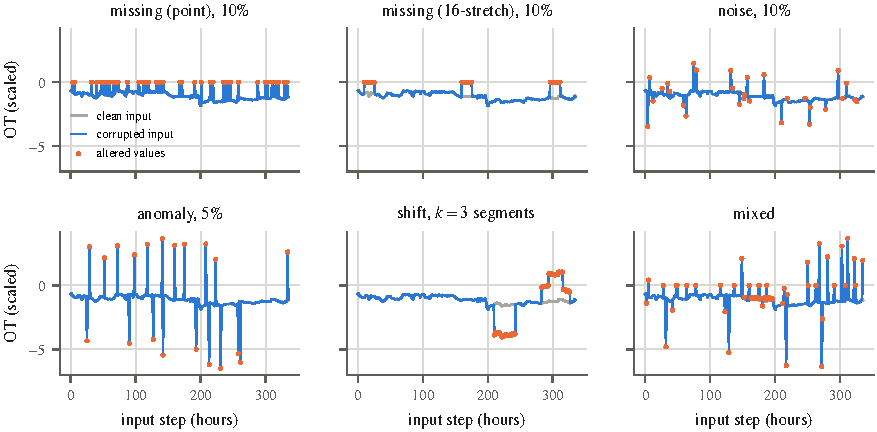
\includegraphics[width=\figwidth]{fig_corruptions.pdf}
\caption{The corruption types applied to one ETTh1 test input window (oil temperature channel, scaled units). Grey: clean input; blue: corrupted input; orange dots: altered values. The panels were drawn with a NumPy port of the project's corruption functions using the same distributions and parameters.}
\label{fig:corr}
\end{figure*}

\subsection{Corruption-Aware Training}
\label{sec:method-cat}

During training each window in a mini-batch is corrupted independently with probability $0.5$ (Fig.~\ref{fig:cat}). For a corrupted window the type is drawn uniformly from \{missing, noise, anomaly, shift\} and the level index uniformly from the four levels; a missing-value corruption is point-wise or stretch-wise with equal probability. The mixed setting is never used for training. The loss~\eqref{eq:mse} is always computed against the clean future, so the network learns to forecast the true continuation from damaged evidence. Because corruption is drawn afresh at every step, the model sees a different damaged copy of each window in every epoch.

\begin{figure}[!t]
\centering
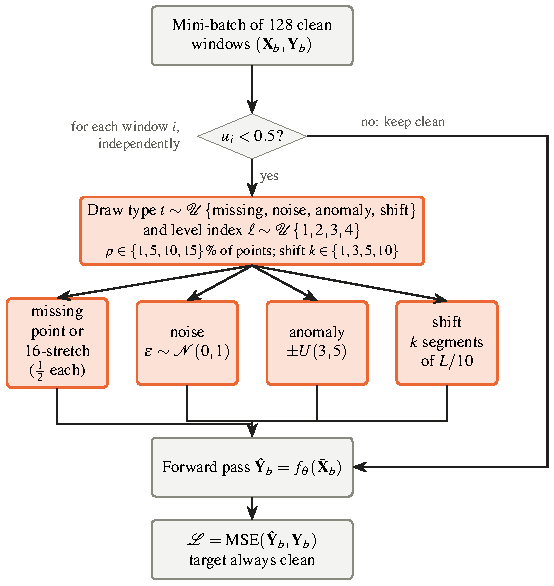
\includegraphics[width=\colfig]{fig_cat.pdf}
\caption{Corruption-aware training. Each window of a mini-batch is corrupted with probability 0.5 using a randomly chosen type and severity. The forecasting loss always uses the clean target.}
\label{fig:cat}
\end{figure}

\subsection{Optimization and Model Selection}
\label{sec:method-opt}

All variants use Adam~\cite{adam} with an initial learning rate $\eta_0=10^{-4}$, batch size 128 and the step decay of the official code (its ``type3'' schedule),
\begin{equation}
\eta_e=\eta_0\cdot0.9^{\max(0,\,e-4)},\qquad e=1,2,\dots
\label{eq:lr}
\end{equation}
Training runs for at most 20 epochs. After each epoch we evaluate the validation MSE on clean windows and on a fixed mixed-corruption copy of the validation set, and keep the checkpoint that minimizes
\begin{equation}
J=\tfrac12\big(\mathrm{MSE}_{\mathrm{val}}^{\mathrm{clean}}+\mathrm{MSE}_{\mathrm{val}}^{\mathrm{mixed}}\big).
\label{eq:select}
\end{equation}
Early stopping uses the same criterion with patience 5. We also keep the checkpoint with the lowest clean validation MSE, which is used only to report the clean reproduction of PatchTST. Algorithm~\ref{alg:train} summarizes the procedure.

\begin{algorithm}[!t]
\caption{Training and selection of one RA-PatchTST variant}
\label{alg:train}
\small
\begin{algorithmic}[1]
\Require training windows $\mathcal{D}_{\mathrm{tr}}$, validation windows $\mathcal{D}_{\mathrm{va}}$, variant flags (gate, shift head, CAT), seed
\State $\tilde{\mathcal{D}}_{\mathrm{va}}\gets$ mixed corruption of $\mathcal{D}_{\mathrm{va}}$ with seed 777
\State initialize $\theta$; gate output bias $c_2\gets4$; $J^\star\gets\infty$; $bad\gets0$
\For{$e=1$ \textbf{to} $20$}
  \State $\eta\gets10^{-4}\cdot0.9^{\max(0,e-4)}$
  \For{each mini-batch $(\X_b,\Y_b)$ of 128 windows, shuffled, last partial batch dropped}
    \If{CAT} \State $\X_b\gets$ corrupt each window with probability 0.5 (random type and level) \EndIf
    \State $\hat{\Y}_b\gets f_\theta(\X_b)$ \Comment{Eqs.~\eqref{eq:revin}--\eqref{eq:shifthead}}
    \State $\theta\gets\mathrm{Adam}\big(\theta,\nabla_\theta\,\mathrm{MSE}(\hat{\Y}_b,\Y_b),\eta\big)$
  \EndFor
  \State $J\gets\frac12\big(\mathrm{MSE}(f_\theta,\mathcal{D}_{\mathrm{va}})+\mathrm{MSE}(f_\theta,\tilde{\mathcal{D}}_{\mathrm{va}})\big)$
  \If{$J<J^\star$} \State $J^\star\gets J$;\ $\theta^\star\gets\theta$;\ $bad\gets0$ \Else \State $bad\gets bad+1$ \EndIf
  \If{$bad\ge5$} \textbf{break} \EndIf
\EndFor
\State \Return $\theta^\star$
\end{algorithmic}
\end{algorithm}

\subsection{Model Variants}
\label{sec:method-variants}

The ablation adds one component at a time (Table~\ref{tab:variants}). A0 is the PatchTST baseline. A1 adds corruption-aware training only, so it isolates the effect of the training data. A2 and A3 add the shift-aware head and the gate respectively on top of A1, and A4 is the full RA-PatchTST. Two further variants are defined in the code, A5 (A4 without corruption-aware training) and A6 (A4 with a gate that does not see the shift features), but they were not run and no result is reported for them.

\begin{table}[!t]
\centering
\caption{Model Variants of the Ablation}
\label{tab:variants}
\footnotesize
\colfit{%
\begin{tabular}{@{}lcccrl@{}}
\toprule
Variant & CAT & Shift head & Gate & Params & Status \\
\midrule
A0 PatchTST & -- & -- & -- & 81,728 & run, 2 seeds \\
A1 & \checkmark & -- & -- & 81,728 & run, 2 seeds \\
A2 & \checkmark & \checkmark & -- & 81,920 & run, 2 seeds \\
A3 & \checkmark & -- & \checkmark & 82,529 & run, 2 seeds \\
A4 RA-PatchTST & \checkmark & \checkmark & \checkmark & 82,721 & run, 2 seeds \\
A5 & -- & \checkmark & \checkmark & 82,721 & defined, not run \\
A6 & \checkmark & \checkmark & \checkmark$^{\dagger}$ & 82,657 & defined, not run \\
\bottomrule
\multicolumn{6}{@{}p{0.95\linewidth}@{}}{\scriptsize CAT: corruption-aware training. $^{\dagger}$Gate without the two shift features (21 inputs instead of 23).}
\end{tabular}}
\end{table}

\subsection{Complexity}
\label{sec:method-complexity}

For a batch of $B$ windows, self-attention costs $O(B\,C\,N^2 D)$ per layer and the feed-forward network $O(B\,C\,N\,D\,d_{ff})$. The gate adds $O(B\,C\,N\cdot(23\cdot32+32))$ operations, roughly the cost of one extra feed-forward layer of width 32 on the patch tokens, and the shift head adds $O(B\,C\,H)$. Neither changes the asymptotic cost. The parameter count of the backbone breaks down as follows: patch embedding 272, position encoding 672, three encoder layers of 5,392 each (attention projections 1,088, two BatchNorms 64, feed-forward 4,240) and the head 64,608, for 81,728 in total. The head dominates, and the gate and shift head together add 993 parameters (1.2\%).

\section{System Architecture}
\label{sec:arch}

The system has two parts: a Python research pipeline that prepares the data, corrupts inputs, trains and evaluates the variants and produces the reports, and a self-contained browser application that runs the trained baseline and RA-PatchTST side by side. Fig.~\ref{fig:pipeline} shows how data move through the pipeline.

\begin{figure*}[!t]
\centering
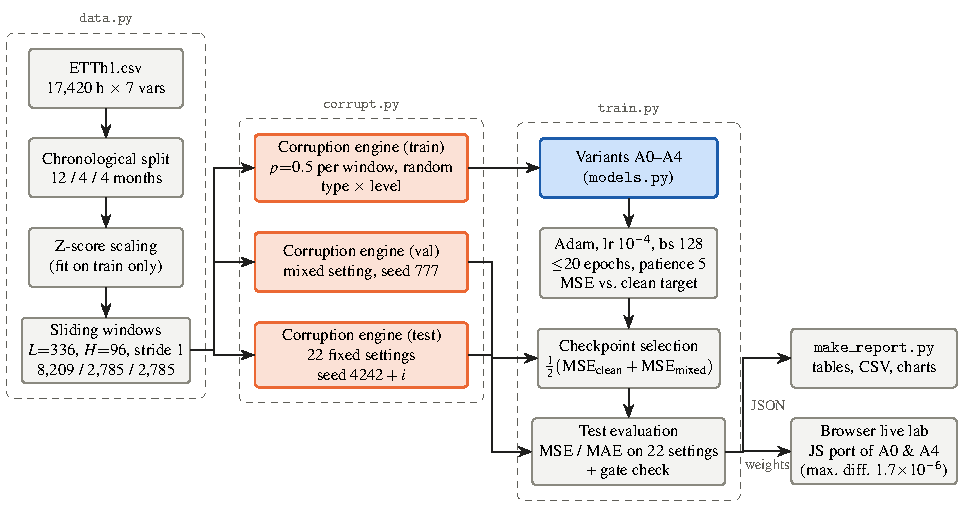
\includegraphics[width=0.92\textwidth]{fig_pipeline.pdf}
\caption{End-to-end pipeline. The same corruption engine produces random corruptions during training, one fixed mixed corruption of the validation set for model selection, and 22 fixed, seeded corruptions of the test set. Results are written as JSON files from which every table and chart is generated; the weights of A0 and A4 are exported to the browser application.}
\label{fig:pipeline}
\end{figure*}

\subsection{Module Design}

The code base consists of five Python modules with narrow interfaces (Table~\ref{tab:modules}). The data module returns tensors only and knows nothing about corruption. The corruption engine is a set of pure functions that take a scaled batch and a seeded random generator and return the corrupted batch together with the mask of altered positions; the same functions serve training, validation and testing, so the corruption seen in evaluation is guaranteed to be the one described in Section~\ref{sec:method-corrupt}. The model module defines a single class whose constructor flags switch the gate and the shift head on or off, and a table that maps each variant name to its flags. The training module owns optimization, selection, evaluation and the gate check, and writes one JSON file per (variant, seed). The report module reads only those JSON files.

\begin{table*}[!t]
\centering
\caption{Software Modules, Responsibilities and Interfaces}
\label{tab:modules}
\footnotesize
\renewcommand{\arraystretch}{1.15}
\begin{tabular}{@{}p{0.14\textwidth}p{0.42\textwidth}p{0.38\textwidth}@{}}
\toprule
Module & Responsibility & Input $\rightarrow$ output \\
\midrule
\texttt{data.py} & Chronological split, train-only scaling, sliding windows, training statistics & CSV file $\rightarrow$ train/val/test tensors, $\bar{\mu}_c,\bar{\sigma}_c$ \\
\texttt{corrupt.py} & Five corruption types, 22 test settings, training-time corruption, patch masks & window batch, seed $\rightarrow$ corrupted batch, mask \\
\texttt{models.py} & PatchTST backbone, reliability gate, shift head; variants A0 to A6 & window batch $\rightarrow$ forecast (and gate weights) \\
\texttt{train.py} & Training loop, checkpoint selection, resumable per-epoch checkpoints, test sweep, gate check & variant, seed $\rightarrow$ result JSON \\
\texttt{make\_report.py} & Aggregation over seeds, tables and charts & result JSON files $\rightarrow$ Markdown, CSV, PNG \\
Live lab (HTML) & JavaScript forward pass of A0 and A4 with embedded weights and test windows & user edits $\rightarrow$ two forecasts, errors, gate weights \\
\bottomrule
\end{tabular}
\end{table*}

\subsection{Tensor Flow Through the Model}

Table~\ref{tab:shapes} traces the shape of the data through one forward pass for a batch of $B$ windows. Channel independence is implemented by folding the channel axis into the batch axis before the encoder and unfolding it before the head; the gate and shift features are computed per channel before folding.

\begin{table}[!t]
\centering
\caption{Tensor Shapes in One Forward Pass}
\label{tab:shapes}
\footnotesize
\colfit{%
\begin{tabular}{@{}ll@{}}
\toprule
Stage & Shape \\
\midrule
Input window $\X$ & $(B,\ 336,\ 7)$ \\
Window statistics $\mu,\sigma$; shift numbers $s^{\mu},s^{\sigma}$ & $(B,\ 7)$ each \\
Patches $\mathbf{p}$ & $(B,\ 7,\ 42,\ 16)$ \\
Gate input $\mathbf{g}$ / gate weights $w$ & $(B,\ 7,\ 42,\ 23)$ / $(B,\ 7,\ 42)$ \\
Embeddings $\mathbf{u}^{(0)}$ (channels folded) & $(7B,\ 42,\ 16)$ \\
Encoder output & $(7B,\ 42,\ 16)$ \\
Head input $[\mathbf{h}_c;s^{\mu}_c;s^{\sigma}_c]$ & $(B,\ 7,\ 674)$ \\
Forecast $\hat{\Y}$ & $(B,\ 96,\ 7)$ \\
\bottomrule
\end{tabular}}
\end{table}

\subsection{Evaluation Subsystem}

Evaluation is deterministic by design. Test setting $i$ ($i=0,\dots,21$) is generated once from the clean test windows with generator seed $4242+i$, and the validation mixed set with seed 777, so all variants and seeds are scored on identical corrupted inputs. For the gated variants the evaluation also reads the gate weights for seven representative settings and splits them by a patch-level mask: a patch counts as corrupted if any of its 16 values was altered, computed by padding and unfolding the position mask exactly as the input is patched.

\subsection{Interactive Live Laboratory}

The live laboratory is a single HTML file that needs no server or network connection. It contains a JavaScript port of the forward pass of A0 and A4 (seed 2021), their trained weights, and a fixed set of 24 ETTh1 test windows. A user picks a window and a channel, applies damage through presets (missing stretches, noise, spikes, level and scale shifts, mixed) or by dragging individual readings, and sees the true future, both forecasts, the damaged input and the trust that the A4 gate gives each patch. A benchmark button runs both models on all $24\times7=168$ sample series under the current damage settings. A dashboard tab shows the experimental results of Section~\ref{sec:results} and states their limitations. When the page was built, the JavaScript forward pass was compared with PyTorch on sample windows and differed by at most $1.7\times10^{-6}$.

\section{Implementation}
\label{sec:impl}

\subsection{Environment}

The system is written in Python~3 with PyTorch~\cite{pytorch}, NumPy and pandas, and matplotlib for the charts. All experiments ran on a cloud CPU container with two virtual cores (Intel Xeon class, 2.1~GHz). Training used two worker processes with one thread each, running the (variant, seed) jobs in a fixed priority order; the script skips jobs whose result file already exists and saves a checkpoint after every epoch, so an interrupted schedule resumes where it stopped. No GPU was used, and a laptop CPU is sufficient to reproduce every run at roughly 40~s per epoch.

\subsection{Hyperparameters}

Table~\ref{tab:hparams} lists every setting. The backbone values are those of the official PatchTST script for ETTh1. No hyperparameter search was carried out for any variant; all variants share the same settings and training budget, so differences between them are attributable to the components being ablated and to seed variation.

\begin{table}[!t]
\centering
\caption{Hyperparameters (Identical for All Variants)}
\label{tab:hparams}
\footnotesize
\colfit{%
\begin{tabular}{@{}ll@{}}
\toprule
Setting & Value \\
\midrule
Look-back $L$ / horizon $H$ & 336 / 96 \\
Patch length $P$ / stride $S$ / patches $N$ & 16 / 8 / 42 \\
Encoder layers / heads / $D$ / FFN width & 3 / 4 / 16 / 128 \\
Dropout & 0.3 \\
Gate hidden width / output bias init. & 32 / $+4$ \\
Gate input clamp & $[-10,10]$ \\
Optimizer / initial learning rate & Adam / $10^{-4}$ \\
Learning-rate decay & $\times0.9$ per epoch after epoch 4 \\
Batch size & 128 (last partial batch dropped) \\
Max.\ epochs / early-stopping patience & 20 / 5 \\
Corruption probability in training & 0.5 per window \\
Training seeds & 2021, 2022 \\
Validation / test corruption seeds & 777 / $4242+i$ \\
Gate penalty $\lambda$ & 0 (not used) \\
\bottomrule
\end{tabular}}
\end{table}

\subsection{Faithfulness to the Official PatchTST}

The backbone was re-implemented from the official code~\cite{patchtst_code} rather than imported, so that the gate and shift head could be inserted at the exact points shown in Fig.~\ref{fig:arch}. It reproduces instance normalization without affine parameters, end padding, patch length 16 with stride 8, the learnable position encoding initialized uniformly in $[-0.02,0.02]$, post-norm encoder layers with BatchNorm, residual attention scores and GELU, and the flatten-linear head. Three small deviations were made, all documented with the code:
\begin{enumerate}
\item dropout is implemented with a uniform random mask ($\mathbf{x}\odot\mathbb{1}[\mathbf{u}\ge p]/(1-p)$, $\mathbf{u}\sim\mathcal{U}(0,1)$), which is mathematically the same inverted dropout but about twice as fast on the CPU;
\item the gate input is clamped to $[-10,10]$ to keep spikes from saturating the gate MLP;
\item the checkpoint used for corrupted-data results is chosen by the combined criterion~\eqref{eq:select} instead of clean validation loss alone, and the clean-validation checkpoint is kept separately for the reproduction check.
\end{enumerate}
The training budget is also smaller than the official one (20 epochs instead of up to 100), which is discussed with the results.

\subsection{Verification}

Before the experiments, the pipeline was checked with the tests in Table~\ref{tab:tests}. They confirm the split sizes, that scaling uses training statistics only, that corruption is deterministic for a given seed and touches only masked positions, that parameter counts match the design, that the untrained gate starts near one, that saved weights reproduce the stored results, and that the browser port agrees with PyTorch.

\begin{table*}[!t]
\centering
\caption{Verification Tests and Their Outcomes}
\label{tab:tests}
\footnotesize
\renewcommand{\arraystretch}{1.12}
\begin{tabular}{@{}lp{0.19\textwidth}p{0.22\textwidth}p{0.18\textwidth}p{0.24\textwidth}l@{}}
\toprule
ID & Purpose & Input & Expected & Observed & Result \\
\midrule
T1 & Window counts & ETTh1, $L=336$, $H=96$ & 8,209 / 2,785 / 2,785 & 8,209 / 2,785 / 2,785 & Pass \\
T2 & Train-only scaling & Training split & Mean 0, std 1 per variable & 0.0 and 1.0 for all 7 variables & Pass \\
T3 & Deterministic corruption & Mixed corruption, seed 4242 twice, then 4243 & Same seed identical; different seed differs & Identical; differs & Pass \\
T4 & Only masked values change & Missing, noise, spike, shift on 128 windows & Unmasked values unchanged & Unchanged for all four; 9.9\% altered at the 10\% level & Pass \\
T5 & Parameter counts & A0, A4, gate & 81,728 / 82,721 / 801 & 81,728 / 82,721 / 801 & Pass \\
T6 & Untrained gate near 1 & A4, untrained, 32 windows & $\approx0.98$ & 0.984 & Pass \\
T7 & Saved weights reproduce results & A0 and A4, seed 2021, clean and mixed test MSE & Match result files & 0.3785/0.4491 (A0), 0.3815/0.4276 (A4) & Pass \\
T8 & Browser port matches PyTorch & Sample windows & Max.\ difference $<10^{-5}$ & $1.7\times10^{-6}$ & Pass \\
T9 & Baseline reproduces paper & ETTh1, $H=96$ & Within 2\% of 0.375 & 0.379 ($+1.1\%$) & Pass \\
\bottomrule
\end{tabular}
\end{table*}

\subsection{Reproducibility}

All randomness is seeded. The training seed fixes model initialization, batch order and, through a separate generator offset by 1000, the training-time corruption. Corrupted evaluation sets use their own fixed seeds. The public ETTh1 file is used unchanged. Every number in Section~\ref{sec:results} is computed by script from the per-run JSON files, which also store the per-epoch training history; the tables and figures of this paper were regenerated from those files.

\section{Experimental Setup}
\label{sec:exp}

\subsection{Dataset}

ETTh1 is the hourly subset of the Electricity Transformer Temperature dataset introduced with Informer~\cite{informer} and distributed through the ETDataset repository~\cite{ettdata} and the Time-Series-Library~\cite{tslib_code}. The file covers 1 July 2016 to 26 June 2018 (17,420 hourly records) from one power transformer in China. It has seven variables: six load features (high, middle and low useful and useless load: HUFL, HULL, MUFL, MULL, LUFL, LULL) and the oil temperature OT. We found no missing values, no duplicate timestamps and no gaps in the hourly spacing. The load features contain negative values and large excursions (HUFL ranges from $-22.7$ to $23.6$), which we keep because they are part of the recorded signal. The data contain no personal information.

Following the standard protocol, the first 12 months form the training set, the next four months the validation set and the following four months the test set; the remaining 3,020 hours are not used. Table~\ref{tab:split} gives the periods and window counts, and Fig.~\ref{fig:dataset} shows two of the variables with the split. The test period falls in winter. Its mean oil temperature is 4.85 against 17.13 in the training year, and the standard deviation of HUFL is 7.66 against 5.81, so even the clean test set is shifted relative to training. Because windows are cut with stride 1, neighbouring samples overlap and are not independent.

\begin{table}[!t]
\centering
\caption{Chronological Split of ETTh1}
\label{tab:split}
\footnotesize
\colfit{%
\begin{tabular}{@{}llr@{}}
\toprule
Split & Period (hourly records) & Windows ($L{=}336$, $H{=}96$) \\
\midrule
Train & 2016-07-01 to 2017-06-25 (8,640) & 8,209 \\
Validation & 2017-06-26 to 2017-10-23 (2,880) & 2,785 \\
Test & 2017-10-24 to 2018-02-20 (2,880) & 2,785 \\
\bottomrule
\end{tabular}}
\end{table}

\begin{figure*}[!t]
\centering
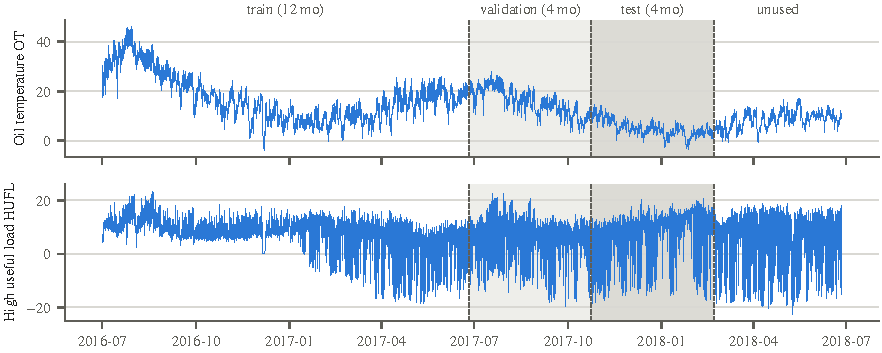
\includegraphics[width=\figwidth]{fig_dataset.pdf}
\caption{Two ETTh1 variables over the full recording with the chronological split. The shaded regions are the validation and test periods; the last 3,020 hours are not used.}
\label{fig:dataset}
\end{figure*}

\subsection{Test Conditions}

Each model is evaluated on 22 versions of the 2,785 test windows (Table~\ref{tab:settings}): the clean inputs, four severity levels for each of the five corruption families, and the mixed setting. Only the input windows are corrupted; the target is the clean future in every case. The mixed setting combines all four training families but at a fixed combination never seen during training.

\begin{table}[!t]
\centering
\caption{The 22 Test Conditions}
\label{tab:settings}
\footnotesize
\renewcommand{\arraystretch}{1.12}
\colfit{%
\begin{tabular}{@{}p{0.28\linewidth}p{0.36\linewidth}p{0.24\linewidth}@{}}
\toprule
Family & Parameters & Levels \\
\midrule
Clean & none & 1 \\
Missing (point) & fraction $p$ of values set to 0 & $p\in\{1,5,10,15\}\%$ \\
Missing (16-stretch) & stretches of 16 zeros, coverage $\approx p$ & $p\in\{1,5,10,15\}\%$ \\
Noise & $+\mathcal{N}(0,1)$ on fraction $p$ & $p\in\{1,5,10,15\}\%$ \\
Anomaly (spike) & $\pm\,\mathcal{U}(3,5)$ on fraction $p$ & $p\in\{1,5,10,15\}\%$ \\
Shift & $k$ segments of 33 steps, $\alpha\!\sim\!\mathcal{U}(0.5,2)$, $\beta\!\sim\!\mathcal{U}(-2,2)$ & $k\in\{1,3,5,10\}$ \\
Mixed & shift $k{=}1$ + noise, spike, missing at 5\% each & 1 \\
\bottomrule
\end{tabular}}
\end{table}

\subsection{Metrics}

We report the mean squared error and mean absolute error on the scaled data,
\begin{equation}
\begin{gathered}
\mathrm{MSE}=\frac{1}{|\mathcal{T}|HC}\sum_{\mathcal{T}}\sum_{i=1}^{H}\sum_{c=1}^{C}(\hat{y}_{i,c}-y_{i,c})^2,\\
\mathrm{MAE}=\frac{1}{|\mathcal{T}|HC}\sum_{\mathcal{T}}\sum_{i=1}^{H}\sum_{c=1}^{C}|\hat{y}_{i,c}-y_{i,c}|,
\end{gathered}
\label{eq:metrics}
\end{equation}
where $\mathcal{T}$ is the set of test windows; lower is better for both. Scaled units make the numbers comparable with published ETTh1 results. Results are aggregated by family (mean over the four levels) and as the mean over all 21 corrupted conditions. Relative change against a reference variant is $\Delta=100\,(\mathrm{MSE}_{v}/\mathrm{MSE}_{\mathrm{ref}}-1)\%$, computed from seed-averaged values, so negative values mean improvement. Gate behaviour is measured as the mean gate weight over corrupted and over clean patches.

\subsection{Statistical Treatment}

Each variant was trained with two seeds (2021 and 2022). We report means with the sample standard deviation over the two seeds, the per-seed values for the headline numbers, and a paired comparison of each variant with A1 in each seed. Two seeds and overlapping test windows do not support formal significance tests or confidence intervals, so we do not report any; the standard deviations should be read as indicating the spread between two runs, nothing more.

\subsection{Baselines}

The baseline is our PatchTST re-implementation (A0). No other published method was re-run under this protocol, so the paper makes no claim about RA-PatchTST relative to DLinear, iTransformer, SEER, TFPS, APT or any other model.

\section{Results and Discussion}
\label{sec:results}

All results are on the ETTh1 test split (2,785 windows, horizon 96, scaled units) and are means over two seeds unless stated otherwise. Table~\ref{tab:headline} gives the headline comparison between the baseline and the full model with the per-seed values; Tables~\ref{tab:groups-mse} to~\ref{tab:delta-a1} break the results down by corruption family and variant, and Appendix~\ref{app:full} lists every condition.

\begin{table}[!t]
\centering
\caption{Headline Results: PatchTST (A0) Versus RA-PatchTST (A4)}
\label{tab:headline}
\footnotesize
\colfit{%
\begin{tabular}{@{}llccl@{}}
\toprule
Model & Test condition & MSE & MAE & Per-seed MSE \\
\midrule
\tabin{tab_headline}
\bottomrule
\end{tabular}}
\end{table}

\subsection{Clean-Data Reproduction (O1)}

Table~\ref{tab:repro} reports the clean test error of each variant with the checkpoint chosen on clean validation loss, which is how PatchTST is usually evaluated. The baseline A0 reaches MSE 0.3791 and MAE 0.4008, against 0.375 and 0.399 published for PatchTST/42~\cite{patchtst}, a gap of 1.1\% in MSE and 0.5\% in MAE, which meets the 2\% target. The remaining gap is plausibly due to the shorter training budget: seed 2021 of A0 reached its best validation score in the last allowed epoch (Table~\ref{tab:cost}), so it had not finished improving. In every run the two checkpoint rules happened to select the same epoch, so the clean numbers in Tables~\ref{tab:headline} and~\ref{tab:repro} coincide.

\begin{table}[!t]
\centering
\caption{Clean Test Error With the Clean-Validation Checkpoint, Against the Published PatchTST/42 Result (MSE 0.375, MAE 0.399)}
\label{tab:repro}
\footnotesize
\colfit{%
\begin{tabular}{@{}lcccc@{}}
\toprule
Variant & MSE & MAE & $\Delta$MSE vs.\ paper & $\Delta$MAE vs.\ paper \\
\midrule
\tabin{tab_repro}
\bottomrule
\end{tabular}}
\end{table}

\subsection{How Much Does Corruption Hurt PatchTST? (RQ1)}

The baseline degrades very unevenly across corruption families (first column of Table~\ref{tab:groups-mse}, Fig.~\ref{fig:groups}). Point-wise missing values, 16-step stretches and noise raise its MSE by only 0.005 to 0.013 on average, and even at 15\% the worst of them costs 7\% (missing stretches, 0.406). Spikes raise the mean MSE to 0.458 ($+20.9\%$) and segment-level shift to 0.520 ($+37.1\%$); at ten shifted segments the MSE reaches 0.712, 88\% above the clean value. Averaged over all 21 corrupted conditions the baseline loses 13.3\%.

Instance normalization explains most of this pattern. A zero in a scaled series is the training mean, which instance normalization turns into a moderate value, and Gaussian noise of one standard deviation on a few percent of the points barely changes the window statistics. A spike of 3 to 5 standard deviations, on the other hand, inflates $\sigma_c$ in~\eqref{eq:revin}, which compresses every other value of the window after normalization and then stretches the forecast when the statistics are restored. A shifted segment moves both $\mu_c$ and $\sigma_c$ and changes the local shape that the patches encode. In both cases the damage spreads, through the window statistics, to every patch of the window.

\begin{table*}[!t]
\centering
\caption{Test MSE by Corruption Family (Mean $\pm$ Standard Deviation Over Two Seeds; Best in Bold)}
\label{tab:groups-mse}
\footnotesize
\begin{tabular}{@{}lccccc@{}}
\toprule
Test condition & A0 PatchTST & A1 +CAT & A2 +CAT+shift head & A3 +CAT+gate & A4 RA-PatchTST \\
\midrule
\tabin{tab_groups_mse}
\bottomrule
\end{tabular}
\end{table*}

\begin{table*}[!t]
\centering
\caption{Test MAE by Corruption Family (Mean $\pm$ Standard Deviation Over Two Seeds; Best in Bold)}
\label{tab:groups-mae}
\footnotesize
\begin{tabular}{@{}lccccc@{}}
\toprule
Test condition & A0 PatchTST & A1 +CAT & A2 +CAT+shift head & A3 +CAT+gate & A4 RA-PatchTST \\
\midrule
\tabin{tab_groups_mae}
\bottomrule
\end{tabular}
\end{table*}

\begin{figure*}[!t]
\centering
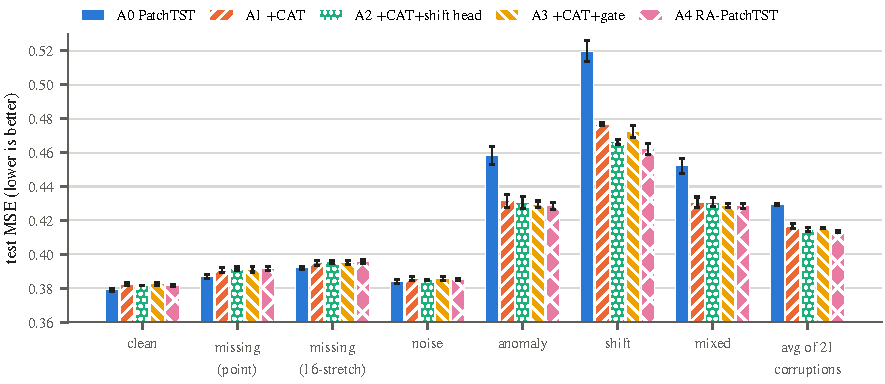
\includegraphics[width=\figwidth]{fig_mse_groups.pdf}
\caption{Test MSE by corruption family for the five variants (mean over two seeds; error bars show the standard deviation between seeds). Note that the vertical axis starts at 0.36.}
\label{fig:groups}
\end{figure*}

\subsection{Effect of RA-PatchTST (RQ2, H1)}

The full model lowers the average MSE over the 21 corrupted conditions from 0.429 to 0.413, a reduction of 3.7\% (Table~\ref{tab:delta-a0}). The reduction is 11.0\% under shift, 6.5\% under spikes and 5.2\% in the mixed setting, and the same ordering holds for MAE (Table~\ref{tab:groups-mae}). The price is a small loss elsewhere: $+0.7\%$ on clean inputs, $+1.3\%$ under point-wise missing values, $+0.9\%$ under missing stretches and $+0.2\%$ under noise. A4 beats A0 in 10 of the 21 corrupted conditions: all four spike levels, all four shift levels, the mixed setting and noise at 15\%. It is worse in the remaining eleven, all of them missing-value or low-level noise conditions where the baseline was already close to its clean error.

The improvement grows with severity (Fig.~\ref{fig:severity}). At one shifted segment A4 is 1.6\% better than A0, at ten segments 20.1\% better (0.569 against 0.712). For spikes the gain rises from 0.6\% at 1\% of points to 11.0\% at 15\%. Fig.~\ref{fig:heatmap} shows the same effect as degradation relative to each model's own clean error: A0 loses 88\% at the worst condition, A4 49\%, and averaged over the 21 conditions A0 loses 13.3\% and A4 8.3\%. For missing values the curves of the three models run nearly parallel, with A0 slightly below.

Against the success criteria of Section~\ref{sec:problem}, A4 lowers the average corrupted MSE in both seeds (0.4132 and 0.4137 against 0.4289 and 0.4298), raises clean MSE by 0.7\% (below the 2\% limit) and adds 1.2\% parameters (below 5\%). H1 is therefore supported on this dataset, with the qualification that the gain is concentrated in two corruption families.

\begin{table}[!t]
\centering
\caption{Change in Test MSE Relative to A0 (Negative Means Better)}
\label{tab:delta-a0}
\footnotesize
\colfit{%
\begin{tabular}{@{}lcccc@{}}
\toprule
Test condition & A1 & A2 & A3 & A4 \\
\midrule
\tabin{tab_delta_a0}
\bottomrule
\end{tabular}}
\end{table}

\begin{figure*}[!t]
\centering
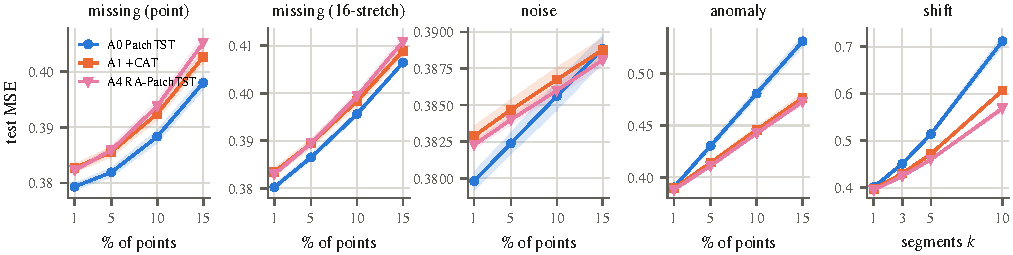
\includegraphics[width=\figwidth]{fig_severity.pdf}
\caption{Test MSE against corruption severity for A0, A1 and A4. Lines are seed means; the shaded bands span the two seeds. Note the different vertical scales.}
\label{fig:severity}
\end{figure*}

\begin{figure*}[!t]
\centering
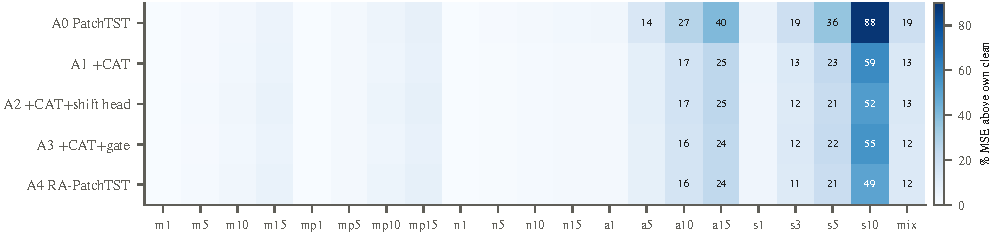
\includegraphics[width=\figwidth]{fig_heatmap.pdf}
\caption{Degradation of each variant relative to its own clean error, $100(\mathrm{MSE}_{\mathrm{cond}}/\mathrm{MSE}_{\mathrm{clean}}-1)$, for the 21 corrupted conditions (m: missing point, mp: missing 16-stretch, n: noise, a: anomaly, s: shift; numbers give the percentage level or the number of shifted segments). Cells of 10\% or more are labelled.}
\label{fig:heatmap}
\end{figure*}

\subsection{Ablation: Where Does the Gain Come From?}

Training on corrupted inputs alone (A1) already gives $-3.0\%$ of the $-3.7\%$ average reduction, that is, about four fifths of the total (Table~\ref{tab:delta-a0}, Fig.~\ref{fig:ablation}). Measured against A1 (Table~\ref{tab:delta-a1}), the shift-aware head (A2) adds $-0.5\%$ on average and $-2.2\%$ under shift, the gate (A3) adds $-0.3\%$ and $-0.9\%$, and the two together (A4) add $-0.8\%$ and $-3.0\%$. The effects of the two components add up almost exactly, which suggests that they address different parts of the problem: the head corrects the level and scale of the forecast, while the gate changes which patches the encoder relies on.

The shift-aware head is the more useful of the two architectural additions, as the analysis of RQ1 would predict: under shift the model needs the window level and scale that instance normalization removes, and the head gives them back. A2 and A4 also reach lower validation errors than A1 and A3 on both the clean and the mixed validation sets (Fig.~\ref{fig:learning}), which points to a benefit that is not limited to the test period.

\begin{table}[!t]
\centering
\caption{Change in Test MSE Relative to A1 (Corruption-Aware Training Only)}
\label{tab:delta-a1}
\footnotesize
\colfit{%
\begin{tabular}{@{}lccc@{}}
\toprule
Test condition & A2 & A3 & A4 \\
\midrule
\tabin{tab_delta_a1}
\bottomrule
\end{tabular}}
\end{table}

\begin{figure}[!t]
\centering
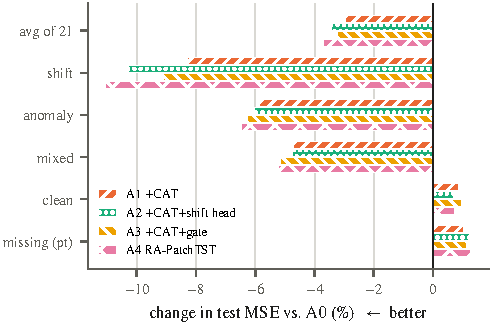
\includegraphics[width=\colfig]{fig_ablation.pdf}
\caption{Change in test MSE relative to A0 for each variant and selected condition groups. Bars to the left of zero are improvements.}
\label{fig:ablation}
\end{figure}

\subsection{Are the Differences Consistent Across Seeds?}

Table~\ref{tab:paired} compares each variant with A1 seed by seed on the average of the 21 corrupted conditions. All three variants improve on A1 in both seeds, and A4 does so by 0.0025 and 0.0039. These differences are small, of the same order as the gap between the two seeds of A1 (0.0020), and with two seeds no significance can be claimed. The comparison with A0 is on firmer ground: the difference between A0 and A4 (0.016) is about 18 times the seed spread of A0 (0.0009) and 32 times that of A4 (0.0005).

\begin{table}[!t]
\centering
\caption{Paired Per-Seed Comparison With A1 on the Average of the 21 Corrupted Conditions}
\label{tab:paired}
\footnotesize
\colfit{%
\begin{tabular}{@{}lcccl@{}}
\toprule
Variant & Seeds & Mean $\Delta$MSE & Seeds better & Per-seed $\Delta$MSE \\
\midrule
\tabin{tab_paired}
\bottomrule
\end{tabular}}
\end{table}

\subsection{Does the Gate Detect Corrupted Patches? (H2)}

Table~\ref{tab:gate} and Fig.~\ref{fig:gate-w} compare the mean gate weight on corrupted and clean patches for seven representative conditions. The gate does react to spikes: in A4 a patch containing a spike receives 0.939 on average, against 0.964 for clean patches in the same windows, and in A3 the gap is wider (0.926 against 0.963). Smaller gaps appear for shift ($-0.017$) and noise ($-0.007$). For missing values, which the zero-share feature was meant to expose, the gate hardly separates damaged from clean patches (a gap of 0.002 to 0.004).

All weights lie between 0.92 and 0.97, so the gate never comes close to switching a patch off; it behaves more like a mild global rescaling with a small extra discount on suspicious patches than like a filter. The gap is also largest for A3, where the gate is the only architectural addition, which suggests that in A4 the shift head takes over part of the work the gate would otherwise do. H2 is supported only weakly, and only for spikes. We therefore do not attribute the robustness of RA-PatchTST mainly to the gate.

\begin{table*}[!t]
\centering
\caption{Mean Gate Weight on Corrupted and Clean Patches (1.0: Fully Trusted). A Patch Counts as Corrupted if Any of Its 16 Values Was Altered}
\label{tab:gate}
\footnotesize
\begin{tabular}{@{}lccccccc@{}}
\toprule
 & & \multicolumn{3}{c}{A3 (+CAT+gate)} & \multicolumn{3}{c}{A4 (RA-PatchTST)} \\
\cmidrule(lr){3-5}\cmidrule(l){6-8}
Condition & Share corrupted & Corrupted & Clean & Gap & Corrupted & Clean & Gap \\
\midrule
\tabin{tab_gate}
\bottomrule
\end{tabular}
\end{table*}

\begin{figure*}[!t]
\centering
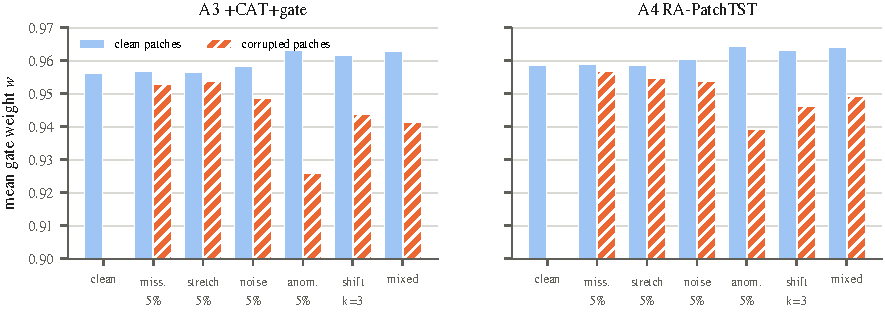
\includegraphics[width=\figwidth]{fig_gate_weights.pdf}
\caption{Mean gate weight on clean and corrupted patches for A3 and A4 (mean over two seeds). The vertical axis spans 0.90 to 0.97: every weight is close to one, and a clear gap appears only for spikes.}
\label{fig:gate-w}
\end{figure*}

\subsection{Training Dynamics}

Fig.~\ref{fig:learning} shows the validation curves. All runs used the full 20 epochs, and the selected checkpoints come from epochs 17 to 20 (Table~\ref{tab:cost}), so none of the models had clearly converged; the official schedule allows up to 100 epochs. On clean validation data A0 ends with the lowest error, as expected for the only model trained on clean data alone. On the mixed validation set the order reverses: at the selected epochs A4 reaches 0.729 to 0.734 and A0 0.761 to 0.765. In every variant the validation MSE is much higher than the test MSE (about 0.68 against 0.38 on clean data), so the two periods differ in difficulty and selection on the validation period transfers to the test period only approximately. Corruption-aware variants also end with higher training loss (0.383 to 0.388 against 0.357 to 0.358 for A0), because half of their training windows are corrupted.

\begin{figure*}[!t]
\centering
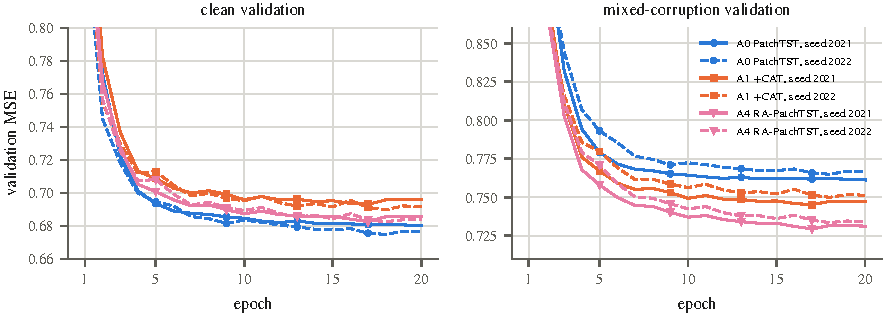
\includegraphics[width=\figwidth]{fig_learning.pdf}
\caption{Validation MSE per epoch for A0, A1 and A4 on clean (left) and mixed-corruption (right) validation windows. Solid lines: seed 2021; dashed lines: seed 2022.}
\label{fig:learning}
\end{figure*}

\subsection{Computational Cost}

Table~\ref{tab:cost} lists the cost of each variant. RA-PatchTST has 993 more parameters than PatchTST (1.2\%), of which 801 are in the gate and 192 in the head. Training time per epoch on one CPU thread rises from 37.0~s to 41.2~s ($+11\%$); 2.0~s of the increase comes from generating corruptions (A1 against A0), 2.0~s from the gate (A3 against A1) and under 1~s from the shift head (A2 against A1). Inference on the 2,785 test windows takes 4.2 to 5.5~s for all variants, and the differences between variants lie within the timing noise of a shared CPU.

\begin{table}[!t]
\centering
\caption{Model Size and Cost (Training Time on One CPU Thread; Inference Over 2,785 Test Windows)}
\label{tab:cost}
\footnotesize
\colfit{%
\begin{tabular}{@{}lrrrccc@{}}
\toprule
Variant & Params & $\Delta$ & Gate & s/epoch & Infer.\ (s) & Sel.\ epoch \\
\midrule
\tabin{tab_cost}
\bottomrule
\multicolumn{7}{@{}l@{}}{\scriptsize Sel.\ epoch: epoch of the selected checkpoint for seeds 2021/2022 (max.\ 20).}
\end{tabular}}
\end{table}

\subsection{Interactive Demonstration}

On the fixed set of 24 test windows $\times$ 7 channels in the live laboratory, with the mixed damage preset, the browser models (seed 2021) give MSE 0.433 for PatchTST and 0.426 for RA-PatchTST ($-1.5\%$), and RA-PatchTST is better on 112 of the 168 series. This is a small demonstration set and not part of the evaluation, but it agrees in direction with the test results.

\subsection{Discussion}

\subsubsection{Interpretation}
The baseline reproduces PatchTST closely and loses accuracy mainly under spikes and shift, in line with the concerns raised about window-local normalization~\cite{fan,apt,revinrole} and patch-level shift~\cite{tfps}. RA-PatchTST reduces these losses, and most of the reduction is due to the training data: a PatchTST that simply sees corrupted windows during training (A1) recovers about 80\% of the gain. The architectural additions help, mostly under shift, and the more effective of them is the simplest one, two numbers appended to the head. The gate learns to discount spikes a little but does not detect missing values.

\subsubsection{Why missing values get slightly worse}
All corruption-aware variants are 0.7 to 1.3\% worse than A0 under missing values and on clean data. Two causes are plausible. First, capacity and training signal are shared: the model spends part of both on spikes and shift, the most damaging families, at a small cost on the mild ones. Second, the zero-filling corruption is easy for the baseline to absorb (a zero is the training mean), so there is little to gain and some precision to lose. The weak response of the gate to missing values may also have a simple cause: the zero-share feature in~\eqref{eq:gatein} is one of 23 inputs, and nothing in the loss rewards the gate for using it.

\subsubsection{Practical significance}
The extra cost is small: 993 parameters, about 11\% more training time and no measurable inference overhead. For data that are mostly clean and complete, RA-PatchTST brings almost no benefit and a slight loss of accuracy. For sensors that are prone to spikes, recalibration jumps or regime changes, the reduction of up to 20\% at high shift severity is a meaningful gain. The model is a research prototype and has not been validated in operation.

\subsubsection{Limitations and threats to validity}
\label{sec:limitations}
The evidence is narrow. Only one dataset (ETTh1), one horizon (96) and one look-back (336) were tested, with two seeds and a 20-epoch budget, and no hyperparameters were tuned. No other published method was re-run, so nothing is claimed relative to SEER~\cite{seer}, TFPS~\cite{tfps}, APT~\cite{apt} or DLinear~\cite{dlinear}. The test corruptions come from the same families that were used in training (only their combination in the mixed setting is new), so the results show robustness to known corruption types, not to unseen ones. The corruptions are synthetic and may differ from real sensor faults. Test windows overlap, so naive confidence intervals would be too narrow. The differences between A2, A3, A4 and A1 are of the same order as the seed variation. Variants A5 and A6 and the gate penalty were not run, so we cannot say how the gate behaves without corruption-aware training or without the shift features. Error analysis by channel or by horizon step was not carried out.

\section{Future Scope}
\label{sec:future}

The limitations above point directly to the next steps, which we order from the most to the least immediate.

\subsubsection{Complete the ablation and strengthen the statistics}
Run at least five seeds per variant, complete A5 (no corruption-aware training) and A6 (gate without shift features), and test the gate penalty $\lambda$. Replace the two-seed standard deviations with confidence intervals from a moving-block bootstrap over test windows~\cite{kunsch}, which respects the overlap between neighbouring windows.

\subsubsection{Broaden the benchmark}
Repeat the protocol on ETTm1, Weather and Electricity and at horizons 192, 336 and 720, with the full training budget of the official code. Re-run DLinear~\cite{dlinear}, iTransformer~\cite{itransformer}, SEER~\cite{seer}, TFPS~\cite{tfps} and APT~\cite{apt} under the same corruption protocol so that the comparison no longer rests on a single baseline.

\subsubsection{Test generalization to unseen damage}
Hold corruption families out of training (for example, train without shift and test with it), add corruption types not modelled here such as stuck-at values, drift ramps and quantization, and evaluate on series with real logged sensor faults rather than synthetic ones.

\subsubsection{Improve the gate}
Give the gate an explicit missing-value mask where the data pipeline can supply one, add a weak auxiliary loss on synthetic corruptions that teaches it where damage is (the corruption engine already produces the mask), and let it act on the attention scores as well as the embeddings. The current result, a gate that stays near one, suggests that the forecasting loss alone gives it too little reason to discriminate.

\subsubsection{Extend the shift signal}
The two shift numbers proved the most useful addition. Richer global descriptors, such as frequency-domain statistics in the spirit of FAN~\cite{fan} or timestamp prototypes as in APT~\cite{apt}, could be passed to the head in the same cheap way, and the effect on clean accuracy should be checked across datasets.

\subsubsection{Towards deployment}
Couple the gate weights with a calibrated uncertainty estimate so that low trust in the input can be reported to an operator, and measure latency on embedded hardware typical of substation monitoring.

\section{Conclusion}
\label{sec:conclusion}

PatchTST gives every input patch the same trust and normalizes away the level and scale of each window, which makes it sensitive to spikes and to shifts in the input. We proposed RA-PatchTST, which adds a patch reliability gate, two shift features for the forecasting head and corruption-aware training, at a cost of 993 parameters, and evaluated it on ETTh1 against a PatchTST re-implementation that reproduces the published clean error to within 1.1\%. Across 21 corrupted test conditions the mean MSE fell from 0.429 to 0.413 ($-3.7\%$), with reductions of 11.0\% under shift, 6.5\% under spikes and 5.2\% under mixed damage, and of 20.1\% at the most severe shift; the clean error rose by 0.7\%.

The ablation qualifies these numbers. Training on corrupted inputs provides about four fifths of the gain. The shift-aware head adds most of the remainder and the gate a little more, and the two effects are additive. The gate discounts spiky patches but does not identify missing values, and its weights stay close to one. The study covers one dataset, one horizon and two seeds, with synthetic corruptions from the training families, so the evidence is preliminary. Within those limits, the results suggest that for patch-based forecasters a large part of the robustness to corrupted inputs can be bought cheaply, through the training data and a global view of shift, and that learning to distrust individual patches needs a stronger signal than the forecasting loss provides.


\section*{Acknowledgment}
The authors thank the Department of Computer Science and Engineering, Ramaiah Institute of Technology, for computing access and guidance. The ETTh1 dataset was released by Zhou \textit{et al.}~\cite{informer} through the ETDataset repository~\cite{ettdata}. The PatchTST re-implementation follows the official code of Nie \textit{et al.}~\cite{patchtst_code}, and the data protocol follows the Time-Series-Library~\cite{tslib_code}.

\bibliographystyle{IEEEtran}
\bibliography{refs}

\appendices
\section{Results for All 22 Test Conditions}
\label{app:full}

Table~\ref{tab:full} gives the test MSE of every variant for every test condition (mean over seeds 2021 and 2022), the MAE of A0 and A4, and the relative change in MSE of A4 against A0. The per-seed values of every run are stored in the result files of the project.

\begin{table*}[!t]
\centering
\caption{Test MSE of All Variants and MAE of A0 and A4 for Every Test Condition (Mean of Two Seeds; Lowest MSE in Bold)}
\label{tab:full}
\footnotesize
\begin{tabular}{@{}lccccccccc@{}}
\toprule
 & \multicolumn{5}{c}{MSE} & \multicolumn{2}{c}{MAE} & \\
\cmidrule(lr){2-6}\cmidrule(lr){7-8}
Condition & A0 & A1 & A2 & A3 & A4 & A0 & A4 & $\Delta$MSE A4 vs.\ A0 \\
\midrule
\tabin{tab_full}
\bottomrule
\end{tabular}
\end{table*}

\section{Data Dictionary}
\label{app:data}

\begin{table}[!h]
\centering
\caption{ETTh1 Variables (Original Units Are Not Stated in the Dataset Documentation)}
\label{tab:dict}
\footnotesize
\colfit{%
\begin{tabular}{@{}llrrrr@{}}
\toprule
Variable & Description & Mean & Std & Min & Max \\
\midrule
HUFL & High useful load & 7.38 & 7.07 & $-22.71$ & 23.64 \\
HULL & High useless load & 2.24 & 2.04 & $-4.76$ & 10.11 \\
MUFL & Middle useful load & 4.30 & 6.83 & $-25.09$ & 17.34 \\
MULL & Middle useless load & 0.88 & 1.81 & $-5.93$ & 7.75 \\
LUFL & Low useful load & 3.07 & 1.16 & $-1.19$ & 8.50 \\
LULL & Low useless load & 0.86 & 0.60 & $-1.37$ & 3.05 \\
OT & Oil temperature (target of interest) & 13.32 & 8.57 & $-4.08$ & 46.01 \\
\bottomrule
\multicolumn{6}{@{}l@{}}{\scriptsize Statistics over all 17,420 records. The \texttt{date} column (hourly timestamps) is dropped before modelling.}
\end{tabular}}
\end{table}

\section{Reproducing the Experiments}
\label{app:repro}

The experiments are reproduced with the commands below, run from the project folder with Python~3, PyTorch, NumPy, pandas and matplotlib installed.

\begin{footnotesize}
\begin{verbatim}
python data.py data_raw/ETTh1.csv
python train.py --variants A0 A1 A2 A3 A4 \
  --seeds 2021 2022 --epochs 20 --patience 5
python make_report.py
\end{verbatim}
\end{footnotesize}

\noindent The first command checks the split shapes, the second trains and evaluates all runs, and the third writes the summary tables and chart.

\noindent \texttt{run\_all.sh} contains the exact two-worker schedule that was used. The figures and tables of this paper are regenerated from the stored result files by \texttt{make\_figures.py} and \texttt{make\_tables.py} in the manuscript repository.


\end{document}
"
\ifdefined\cameraready
  \documentclass[journal]{IEEEtran}
\else
  \documentclass[journal,12pt,onecolumn]{IEEEtran}
\fi

\usepackage{cite}
\usepackage{amsmath,amssymb,amsfonts}
\usepackage{bm}
\usepackage{graphicx}
\usepackage{booktabs}
\usepackage{multirow}
\usepackage{array}
\usepackage{xcolor}
\usepackage{algorithm}
\usepackage{algpseudocode}
\usepackage{textcomp}
\usepackage{url}
\usepackage[hidelinks]{hyperref}
\graphicspath{{figures/}}
\interdisplaylinepenalty=2500

\ifdefined\cameraready
  \newcommand{\figwidth}{\textwidth}
  \newcommand{\colfig}{\columnwidth}
\else
  \newcommand{\figwidth}{0.98\textwidth}
  \newcommand{\colfig}{0.62\textwidth}
\fi

\newcommand{\X}{\mathbf{X}}
\newcommand{\Y}{\mathbf{Y}}
\newcommand{\R}{\mathbb{R}}
\DeclareMathOperator*{\argmin}{arg\,min}

\ifdefined\cameraready
  \newcommand{\colfit}[1]{\resizebox{\columnwidth}{!}{#1}}
\else
  \newcommand{\colfit}[1]{#1}
\fi
\makeatletter\newcommand{\tabin}[1]{\@@input tables/#1.tex }\makeatother
\hyphenation{Patch-TST RA-Patch-TST Trans-former}

\begin{document}

\title{RA-PatchTST: A Reliability-Aware Extension of PatchTST for Multivariate Time-Series Forecasting Under Corrupted Inputs}

\author{Jeevika~N,
        Jnanottam~G~Y,
        and~Mallegowda~M%
\thanks{The authors are with the Department of Computer Science and Engineering, Ramaiah Institute of Technology, MSR Nagar, MSRIT Post, Bengaluru 560054, India. This work was carried out as part of the course Artificial Intelligence and Machine Learning (24CS52), academic year 2026--27.}}

\markboth{RA-PatchTST: Reliability-Aware PatchTST Under Corrupted Inputs}%
{N \MakeLowercase{\textit{et al.}}: RA-PatchTST: Reliability-Aware PatchTST Under Corrupted Inputs}

\maketitle

\begin{abstract}
Patch-based Transformer forecasters such as PatchTST treat every input patch as equally trustworthy, yet sensor series routinely contain missing readings, measurement noise, spikes and shifts in level or scale. This paper presents RA-PatchTST, a reliability-aware extension of PatchTST that adds three small components to the original design: a patch reliability gate (a two-layer perceptron with 801 parameters that scores each patch between 0 and 1 and rescales its embedding), a shift-aware forecasting head that receives the mean and scale of each input window relative to the training statistics, which instance normalization would otherwise discard, and corruption-aware training, in which half of the training windows are corrupted on the fly while the loss is always computed against the clean future. The full model adds 993 parameters (1.2\%) to an 81,728-parameter backbone. We evaluate on the ETTh1 benchmark (17,420 hourly records, seven variables, chronological 12/4/4-month split, look-back 336, horizon 96) using five ablation variants, two random seeds and 22 fixed test conditions: clean data plus 21 seeded corruptions covering point-wise and 16-step missing values, Gaussian noise, spikes, segment-level shift and a mixed setting. Our PatchTST re-implementation reaches a clean test MSE of 0.379 against the published 0.375. RA-PatchTST lowers the mean MSE over the 21 corrupted conditions from 0.429 to 0.413 ($-3.7\%$), with the largest reductions under shift ($-11.0\%$), spikes ($-6.5\%$) and mixed damage ($-5.2\%$), at a cost of $+0.7\%$ on clean data and up to $+1.3\%$ under missing values. The ablation attributes about four fifths of the gain to corruption-aware training; the gate and the shift-aware head add a further $-0.8\%$, concentrated on shift. The gate assigns clearly lower weight to corrupted patches only for spikes. With one dataset, one horizon, two seeds and synthetic corruptions drawn from the training families, these results are preliminary evidence for the approach and do not establish general superiority.
\end{abstract}

\begin{IEEEkeywords}
Time-series forecasting, PatchTST, Transformer, robustness, distribution shift, data corruption, reliability gating, instance normalization, ablation study.
\end{IEEEkeywords}

\section{Introduction}
\label{sec:intro}

\IEEEPARstart{F}{orecasting} the next few days of a multivariate sensor series supports load planning in power networks, scheduling in industrial plants and maintenance of equipment such as power transformers. Deep forecasters for this task have changed quickly over the last five years. Informer~\cite{informer} and its successors Autoformer~\cite{autoformer} and FEDformer~\cite{fedformer} adapted the Transformer~\cite{vaswani} to long sequences. DLinear~\cite{dlinear} then showed that a single linear layer could match or beat these models on the standard long-term benchmarks, and PatchTST~\cite{patchtst} restored the lead of attention-based models by splitting each channel into short overlapping patches, treating each patch as a token and processing channels independently with shared weights. PatchTST is now a common baseline in forecasting studies and in benchmark libraries~\cite{tslib}.

These models are compared on clean benchmarks, while real sensor streams are noisy in several ways: readings go missing when a logger fails, analog channels pick up noise, transient faults produce isolated spikes, and recalibration or a change in operating regime moves a stretch of the series to a different level or scale~\cite{blazquez_anomaly,gama_drift}. In forecasting there are rarely labels that say which inputs are bad~\cite{seer}, so the model has to cope with corrupted inputs without being told where they are.

Two properties of PatchTST make it sensitive to such inputs. First, every patch enters the encoder with the same standing. The attention weights can in principle learn to ignore a damaged patch, but nothing in the architecture or the training signal encourages this. Second, PatchTST normalizes each input window by its own mean and standard deviation (the instance normalization of RevIN~\cite{revin}, without the affine part) and restores those statistics at the output. This helps under slow drift, but it also removes the information that would tell the model that a window sits at an unusual level relative to the training data. Recent analyses argue that window-local statistics cannot capture every kind of shift~\cite{fan,apt,revinrole}.

In our own baseline run, under the segment-level shift corruption described in Section~\ref{sec:exp}, the test MSE of a faithful PatchTST re-implementation on ETTh1 rises from 0.379 on clean inputs to 0.520 on average over four severity levels, and to 0.712 at the highest level. Spikes raise it to 0.458. Missing values and noise, by contrast, cost less than 0.015.

Existing remedies fall into three groups (Section~\ref{sec:lit}). Normalization-based methods such as RevIN~\cite{revin}, Dish-TS~\cite{dishts}, FAN~\cite{fan} and APT~\cite{apt} target distribution shift but do not weigh inputs by quality. Robustness-oriented frameworks such as SEER~\cite{seer}, RobustTSF~\cite{robusttsf} and TameR~\cite{tamer} address noisy or anomalous inputs, but either replace the forecaster with a new architecture, focus on one type of damage, or act only at training time~\cite{tps}. Expert-based and test-time methods such as TFPS~\cite{tfps} and SOLID~\cite{solid} add parameters or per-sample fine-tuning. None of the studies we surveyed offers a small plug-in for PatchTST that scores the reliability of each patch and gives the head a global view of shift within a single forward pass; we make no claim about work outside that set.

This paper studies whether such a plug-in helps, and by how much. We make four contributions.
\begin{enumerate}
\item A reproducible corruption benchmark on ETTh1 with 22 fixed test conditions (clean plus five corruption families at four severity levels and one mixed setting), in which every model sees identical corrupted inputs.
\item RA-PatchTST, which adds to PatchTST a patch reliability gate, two shift features appended to the forecasting head, and corruption-aware training, for 993 extra parameters in total.
\item An ablation over five variants (A0 to A4) and two seeds that separates the contribution of training on corrupted data from that of each architectural component, together with a direct check of whether the gate down-weights corrupted patches.
\item A browser-based live laboratory in which the original and the proposed model run side by side on real ETTh1 test windows that the user can damage interactively.
\end{enumerate}

RA-PatchTST reduces the average corrupted-input MSE by 3.7\% and the shift error by 11.0\%, but most of this gain comes from corruption-aware training, the gate is a weak detector except for spikes, and the model is slightly worse than PatchTST on clean data and under missing values. The PatchTST backbone is a re-implementation of the published design~\cite{patchtst,patchtst_code}; the research contribution lies in the gate, the shift features, their combination with corruption-aware training, and the ablation that measures what each part adds.

The rest of the paper is organized as follows. Section~\ref{sec:lit} reviews related work. Section~\ref{sec:problem} states the problem formally. Section~\ref{sec:method} develops the method, Section~\ref{sec:arch} describes the system architecture and Section~\ref{sec:impl} the implementation. Section~\ref{sec:exp} gives the experimental protocol and Section~\ref{sec:results} the results and their discussion. Sections~\ref{sec:future} and~\ref{sec:conclusion} outline future work and conclude.

\section{Literature Review}
\label{sec:lit}

We carried out a focused narrative review. We searched arXiv, the proceedings of ICLR, ICML, NeurIPS, AAAI and KDD, and the Google Scholar and GitHub pages of the papers found, using the terms \emph{PatchTST}, \emph{patch-based forecasting}, \emph{robust time series forecasting}, \emph{distribution shift}, \emph{instance normalization}, \emph{missing values} and \emph{anomalies}, for the period 2021 to 2026. A study was kept if it builds on or compares with patch-based Transformers, if it addresses corrupted inputs or distribution shift in forecasting, or if it defines the benchmark protocol. Several 2026 entries were preprints at the time of writing. Because the papers use different datasets, horizons and protocols, we do not compare their numbers with ours.

\subsection{From Sequence Transformers to Patch Tokens}

The Transformer~\cite{vaswani} replaced recurrence with self-attention, and Informer~\cite{informer} was among the first to adapt it to long-sequence time-series forecasting, introducing ProbSparse attention and, with it, the ETT datasets that remain a standard benchmark. Autoformer~\cite{autoformer} built series decomposition into the network and replaced point-wise attention with an auto-correlation mechanism, and FEDformer~\cite{fedformer} moved attention into the frequency domain. Zeng \textit{et al.}~\cite{dlinear} then questioned the whole line of work: one-layer linear models with a trend-seasonal split (DLinear) outperformed these Transformers on nine benchmarks, suggesting that point-wise tokens carry too little semantic content for attention to exploit.

PatchTST~\cite{patchtst} answered this by grouping consecutive time steps into patches, in the same spirit as the image patches of the Vision Transformer~\cite{vit}. A look-back of 336 steps cut into patches of 16 with stride 8 gives 42 tokens per channel, which shortens the attention span by a factor of about eight and gives each token local shape information. PatchTST also processes each channel independently with shared weights, and normalizes each input window with its own statistics. The official implementation~\cite{patchtst_code} uses BatchNorm inside the encoder~\cite{batchnorm}, GELU activations~\cite{gelu} and residual attention scores in the style of RealFormer~\cite{realformer}. On ETTh1 with look-back 336 and horizon 96, the supervised PatchTST/42 reports MSE 0.375 and MAE 0.399~\cite{patchtst}.

Later models moved in several directions. TimesNet~\cite{timesnet} reshapes a series into two-dimensional period-by-phase tensors. iTransformer~\cite{itransformer} inverts the token axis and attends across variables instead of time. TimeMixer~\cite{timemixer} mixes seasonal and trend components across scales with MLPs, and xPatch~\cite{xpatch} combines patching with exponential seasonal-trend decomposition in a dual-stream CNN and MLP network. Chronos~\cite{chronos} takes the foundation-model route, scaling and quantizing values into tokens and training a language-model architecture on a large corpus for zero-shot use. The Time-Series-Library survey and benchmark~\cite{tslib,tslib_code} fixes a common protocol for these models, which we follow.

\subsection{Normalization and Distribution Shift}

A forecaster trained on one period and applied to the next faces distribution shift, a problem studied in machine learning under the names dataset shift~\cite{datasetshift} and concept drift~\cite{gama_drift}. RevIN~\cite{revin} handles it by normalizing each input window and restoring its statistics at the output, with optional learnable affine parameters. Non-stationary Transformers~\cite{nstransformer} combine such series stationarization with a de-stationary attention that reinjects the removed statistics into the attention scores, which is the closest prior idea to our shift-aware head. Dish-TS~\cite{dishts} separates the shift within the look-back window from the shift between look-back and horizon. FAN~\cite{fan} argues that mean and variance do not describe non-stationarity in the frequency domain and removes the dominant Fourier components instead. APT~\cite{apt} adds affine prototypes indexed by timestamp because, in its authors' analysis, local mean and variance miss global shift. An analysis of RevIN using PatchTST~\cite{revinrole} finds that some of its parts are redundant or even harmful, and that it does not cover all forms of shift. TS\_Adam~\cite{tsadam} changes the optimizer to cope with drift during training.

Two methods react to shift more actively. TFPS~\cite{tfps} identifies patch-level distribution shift and routes patches to pattern-specific experts in the time and frequency domains. SOLID~\cite{solid} detects context-driven shift and fine-tunes the prediction layer for each test sample on similar training samples, which adds computation at test time just as TFPS adds experts.

\subsection{Robustness to Corrupted Inputs}

Missing values are usually handled by imputation before forecasting, with recurrent models such as BRITS~\cite{brits} or self-attention models such as SAITS~\cite{saits}; anomalies are usually handled by detection~\cite{blazquez_anomaly}. Both add a separate model with its own training and error. Several recent works instead make the forecaster itself tolerant to corruption. RobustTSF~\cite{robusttsf} analyzes forecasting when the training data contain anomalies and proposes a robust training procedure. TameR~\cite{tamer} uses global context to reduce the bias of forecasters toward recent, possibly corrupted, observations and reports gains under noise, missing values and anomalies. SEER~\cite{seer} is the closest work to ours: a Transformer framework with a channel-adaptive module and a learnable patch replacement module that filters low-quality patches, tested under missing values, shifts, anomalies and noise. SEER is a full framework, whereas we ask how much of the benefit a far smaller addition to an unchanged PatchTST can deliver. Temporal Patch Shuffle~\cite{tps} augments training data by shuffling patches and improves the robustness of several model families, PatchTST included, but at test time every patch is still trusted equally.

Our evaluation design borrows from computer vision, where Hendrycks and Dietterich~\cite{hendrycks_corrupt} defined a benchmark of common corruptions at graded severities applied to the test set only. A study of Autoformer, Informer and PatchTST on synthetic signals~\cite{synthbench} similarly compares architectures under controlled noise. Training on corrupted copies of the input is a form of data augmentation, which the survey of Wen \textit{et al.}~\cite{tsaug_survey} reviews for time series.

\subsection{Gating as a Soft Selection Mechanism}

Multiplicative gates with sigmoid outputs are a standard way to let a network decide how much of a signal to pass. LSTM gates~\cite{lstm} control the flow of memory, gated linear units~\cite{glu} modulate convolutional features, and squeeze-and-excitation blocks~\cite{senet} rescale feature channels using a small bottleneck MLP over pooled statistics. Our reliability gate follows the last pattern most closely: a small MLP reads summary statistics of each patch and outputs a scale factor applied to that patch's embedding.

\subsection{Summary and Research Gap}

Table~\ref{tab:lit} summarizes the studies most relevant to this work. Shift-oriented methods change normalization or add experts, but none of them weighs inputs by their quality. The robustness-oriented methods do address corrupted inputs, each in its own way: SEER and TameR with new architectures, RobustTSF with a focus on anomalies, and TPS through augmentation at training time only. The accuracy-oriented models address neither problem. None of them tests how far a few hundred parameters added to an unchanged PatchTST can go, or which of the possible additions helps; Sections~\ref{sec:method} and~\ref{sec:results} take up both questions.

\begin{table*}[!t]
\centering
\caption{Studies Most Relevant to This Work and the Gap Each Leaves Open}
\label{tab:lit}
\footnotesize
\renewcommand{\arraystretch}{1.15}
\begin{tabular}{@{}p{0.17\textwidth}p{0.36\textwidth}p{0.40\textwidth}@{}}
\toprule
Study (venue, year) & Approach & Relevance and limitation for this work \\
\midrule
SEER~\cite{seer} (ICML 2026) & Channel-adaptive module and learnable patch replacement that filters low-quality patches & Closest aim; a full new framework rather than a small add-on to PatchTST \\
APT~\cite{apt} (AAAI 2026) & Affine prototypes indexed by timestamp for shift & Shift only; motivates giving the model global statistics \\
TameR~\cite{tamer} (ICML 2026) & Global context against recent-data bias & Robust to noise, missing values and anomalies; no per-patch reliability score \\
TPS~\cite{tps} (preprint, 2026) & Patch shuffling as training augmentation & Training time only; all patches trusted equally at test time \\
RevIN analysis~\cite{revinrole} (preprint, 2026) & Ablation of RevIN components with PatchTST & Analysis only; supports adding a global view of shift \\
TS\_Adam~\cite{tsadam} (Neurocomputing, 2026) & Optimizer modified for drift & Cannot distinguish reliable from unreliable inputs \\
xPatch~\cite{xpatch} (AAAI 2025) & Dual-stream patching with exponential decomposition & Accuracy-oriented; no input-quality mechanism \\
TFPS~\cite{tfps} (NeurIPS 2025) & Pattern-specific experts for patch-level shift & More parameters; targets shift rather than noise or missing data \\
FAN~\cite{fan} (NeurIPS 2024) & Frequency adaptive normalization & Shift only; does not weigh patches by quality \\
RobustTSF~\cite{robusttsf} (ICLR 2024) & Robust training with anomalous data & Anomalies only; not patch-based \\
SOLID~\cite{solid} (KDD 2024) & Detect context-driven shift, fine-tune per sample & Costly at test time; our gate needs one forward pass \\
iTransformer~\cite{itransformer}, TimeMixer~\cite{timemixer} (ICLR 2024) & Variate tokens; multiscale MLP mixing & Accuracy-oriented baselines \\
Chronos~\cite{chronos} (TMLR 2024) & Pretrained tokenized forecaster & Large pretrained model; not a lightweight fix \\
DLinear~\cite{dlinear} (AAAI 2023) & Linear model with decomposition & Strong simple baseline; no robustness mechanism \\
PatchTST~\cite{patchtst} (ICLR 2023) & Patching, channel independence, instance norm. & Base model; equal trust in all patches, window-local statistics only \\
RevIN~\cite{revin} (ICLR 2022) & Reversible instance normalization & Uses only the window's own mean and variance \\
\bottomrule
\end{tabular}
\end{table*}

\section{Problem Statement}
\label{sec:problem}

\subsection{Forecasting Setting}

Let $\{\mathbf{s}_t\}_{t=1}^{T_{\mathrm{tot}}}$, $\mathbf{s}_t\in\R^{C}$, be a multivariate series with $C$ channels sampled at regular intervals. At time $t$ a forecaster receives the look-back window $\X=[\mathbf{s}_{t-L+1},\dots,\mathbf{s}_t]^{\top}\in\R^{L\times C}$ and predicts the next $H$ steps $\Y=[\mathbf{s}_{t+1},\dots,\mathbf{s}_{t+H}]^{\top}\in\R^{H\times C}$. In this work $C=7$, $L=336$ and $H=96$, so the model reads two weeks of hourly data and forecasts the next four days. A forecaster $f_\theta$ is trained by minimizing the mean squared error
\begin{equation}
\mathcal{L}(\theta)=\mathbb{E}_{(\X,\Y)}\Big[\tfrac{1}{HC}\big\lVert f_\theta(\X)-\Y\big\rVert_F^2\Big].
\label{eq:mse}
\end{equation}

\subsection{Corrupted Inputs}

In deployment the model may receive a corrupted window $\tilde{\X}=\mathcal{C}(\X;\,\kappa,\ell,\xi)$, where $\mathcal{C}$ is a corruption operator of type $\kappa$ (missing values, noise, spike, shift or a mixture), severity $\ell$, and random draw $\xi$. The location of the damage is unknown to the model; we write $\mathbf{M}\in\{0,1\}^{L\times C}$ for the mask of altered positions, which is used only for analysis. The forecast target is never corrupted: the goal is to predict the true future $\Y$ from damaged evidence $\tilde{\X}$. Section~\ref{sec:method-corrupt} defines $\mathcal{C}$ precisely.

\subsection{Problem Definition}

Given a PatchTST forecaster, the problem is to keep the forecast error low when the input is corrupted, with three constraints that make the result usable as a plug-in:
\begin{enumerate}
\item the error on clean inputs should not rise by more than 2\%;
\item the parameter count should not rise by more than 5\%;
\item the model must run in a single forward pass, without a separate imputation or detection model and without test-time adaptation.
\end{enumerate}

\subsection{Research Questions and Hypotheses}

\textit{RQ1:} How much accuracy does a faithful PatchTST lose under controlled input corruption, and which corruption types hurt most?

\textit{RQ2:} Can a reliability gate, a shift-aware head and corruption-aware training reduce that loss, and how much does each contribute?

We test two hypotheses separately.
\begin{itemize}
\item \textbf{H1.} Together, the three components lower the test MSE of PatchTST averaged over the corrupted conditions, while the clean-data MSE changes only slightly.
\item \textbf{H2.} The gate learns to assign lower weight to corrupted patches than to clean patches.
\end{itemize}

\subsection{Objectives and Success Criteria}

Table~\ref{tab:objectives} lists the objectives and how each is measured. The numerical thresholds are practical targets we set for a lightweight add-on, not standards from the literature. The original plan to cover four datasets (ETTh1, ETTm1, Weather, Electricity) and four horizons was reduced to ETTh1 at horizon 96 because all training ran on CPUs; Section~\ref{sec:limitations} returns to this.

\begin{table}[!t]
\centering
\caption{Objectives and Success Criteria}
\label{tab:objectives}
\footnotesize
\renewcommand{\arraystretch}{1.15}
\colfit{%
\begin{tabular}{@{}p{0.06\linewidth}p{0.42\linewidth}p{0.44\linewidth}@{}}
\toprule
ID & Objective & Measure and target \\
\midrule
O1 & Re-implement PatchTST and reproduce its clean ETTh1 result & Test MSE within 2\% of the published 0.375 \\
O2 & Build a seeded corruption benchmark & 22 conditions; identical inputs for all models \\
O3 & Design RA-PatchTST & Parameter increase below 5\% \\
O4 & Compare A0 with variants A1 to A4 & Mean corrupted MSE lower than A0 in every seed; clean MSE increase below 2\% \\
O5 & Check what the gate learns & Mean gate weight on corrupted vs.\ clean patches \\
O6 & Build an interactive demonstration & Browser port agrees with PyTorch within $10^{-5}$ \\
\bottomrule
\end{tabular}}
\end{table}

\section{Proposed Methodology}
\label{sec:method}

RA-PatchTST keeps the PatchTST backbone unchanged and adds three components (Fig.~\ref{fig:arch}). This section first describes data preparation and the backbone, then each addition, the corruption model used for training and testing, and the training objective.

\begin{figure*}[!t]
\centering
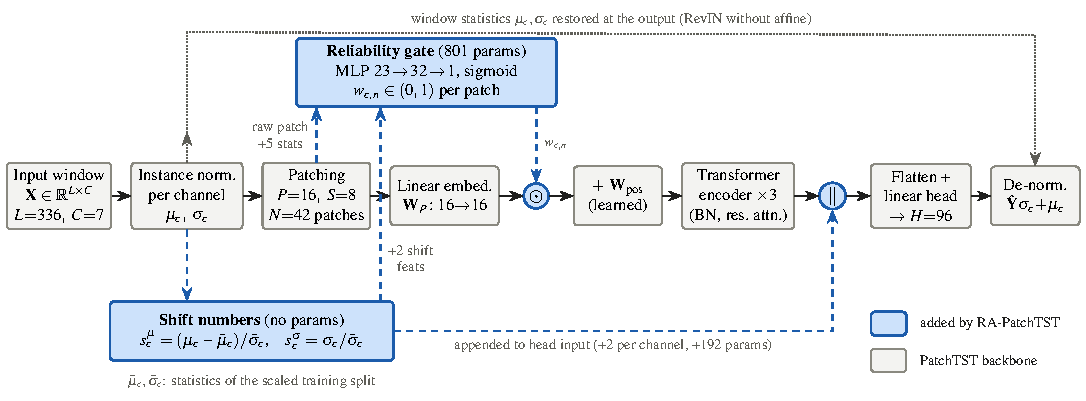
\includegraphics[width=\figwidth]{fig_architecture.pdf}
\caption{RA-PatchTST architecture. Grey blocks are the PatchTST backbone; blue blocks are the components added in this work. The reliability gate scores every patch and rescales its embedding before the position encoding is added; the two shift numbers are computed from the window statistics that instance normalization removes and are appended to the input of the linear head. Corruption-aware training (Fig.~\ref{fig:cat}) changes only the data fed to this network.}
\label{fig:arch}
\end{figure*}

\subsection{Data Preparation}
\label{sec:method-data}

The series is split chronologically into training, validation and test segments (Section~\ref{sec:exp}). A per-channel z-score scaler is fitted on the training segment only and applied to all three,
\begin{equation}
\begin{gathered}
\bar{s}_{t,c}=\frac{s_{t,c}-m_c}{d_c},\qquad m_c=\frac{1}{T_{\mathrm{tr}}}\sum_{t\le T_{\mathrm{tr}}}s_{t,c},\\
d_c^2=\frac{1}{T_{\mathrm{tr}}}\sum_{t\le T_{\mathrm{tr}}}(s_{t,c}-m_c)^2,
\end{gathered}
\label{eq:scale}
\end{equation}
so that no validation or test statistics leak into training. Windows of length $L+H$ are then cut with stride 1. Validation and test windows start $L$ steps before their segment so that the first forecast target lies exactly on the segment border, as in the Time-Series-Library protocol~\cite{tslib_code}. We also store the per-channel mean $\bar{\mu}_c$ and standard deviation $\bar{\sigma}_c$ of the \emph{scaled} training segment, which the shift features use. By construction $\bar{\mu}_c=0$ and $\bar{\sigma}_c=1$ up to rounding; the code keeps them explicit so that the same model can be used with other scalers.

\subsection{PatchTST Backbone}
\label{sec:method-backbone}

\subsubsection{Instance normalization}
For each window and channel the model computes
\begin{equation}
\begin{gathered}
\mu_c=\frac{1}{L}\sum_{i=1}^{L}x_{i,c},\qquad \sigma_c=\sqrt{\frac{1}{L}\sum_{i=1}^{L}(x_{i,c}-\mu_c)^2+\varepsilon},\\
x^{N}_{i,c}=\frac{x_{i,c}-\mu_c}{\sigma_c},
\end{gathered}
\label{eq:revin}
\end{equation}
with $\varepsilon=10^{-5}$. The statistics are treated as constants during back-propagation. This is RevIN~\cite{revin} without the learnable affine parameters, matching the configuration of the official PatchTST script for ETTh1.

\subsubsection{Patching}
Each normalized channel $\mathbf{x}^{N}_{c}\in\R^{L}$ is padded at the end with $S$ copies of its last value and unfolded into overlapping patches of length $P$ with stride $S$ (Fig.~\ref{fig:patching}):
\begin{equation}
\begin{gathered}
\mathbf{p}_{c,n}=\big[x^{N}_{nS+1,c},\dots,x^{N}_{nS+P,c}\big]^{\top}\in\R^{P},\\
n=0,\dots,N-1,\qquad N=\Big\lfloor\frac{L-P}{S}\Big\rfloor+2.
\end{gathered}
\label{eq:patch}
\end{equation}
With $L=336$, $P=16$ and $S=8$ this gives $N=42$ patches per channel, hence the name PatchTST/42.

\begin{figure}[!t]
\centering
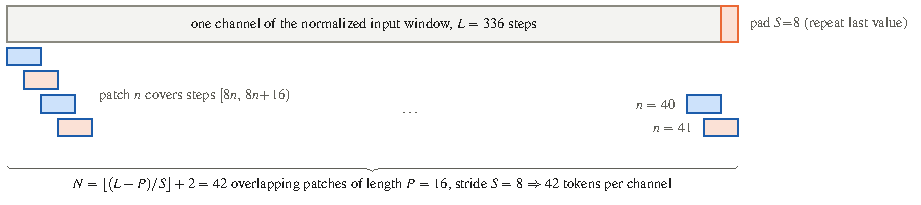
\includegraphics[width=\colfig]{fig_patching.pdf}
\caption{Patching of one channel. End padding with $S$ repeated values adds one patch, giving $N=42$ tokens for $L=336$, $P=16$, $S=8$.}
\label{fig:patching}
\end{figure}

\subsubsection{Embedding and encoder}
Each patch is mapped to a $D$-dimensional token by a shared linear layer, and a learnable position encoding $\mathbf{W}_{\mathrm{pos}}\in\R^{N\times D}$ is added:
\begin{equation}
\mathbf{e}_{c,n}=\mathbf{W}_P\,\mathbf{p}_{c,n}+\mathbf{b}_P,\qquad \mathbf{u}^{(0)}_{c,n}=\mathbf{e}_{c,n}+\mathbf{W}_{\mathrm{pos},n}.
\label{eq:embed}
\end{equation}
Channels are processed independently: the batch of $B$ windows becomes $B\cdot C$ sequences of $N$ tokens. Each of the three encoder layers applies multi-head self-attention with residual attention scores~\cite{realformer}, followed by a position-wise feed-forward network, each wrapped in a residual connection and BatchNorm~\cite{batchnorm}. For head $h$ in layer $l$,
\begin{equation}
\begin{gathered}
\mathbf{A}^{(l)}_h=\frac{\mathbf{Q}^{(l)}_h{\mathbf{K}^{(l)}_h}^{\top}}{\sqrt{d_k}}+\mathbf{A}^{(l-1)}_h,\\
\mathrm{head}^{(l)}_h=\mathrm{softmax}\big(\mathbf{A}^{(l)}_h\big)\,\mathbf{V}^{(l)}_h,
\end{gathered}
\label{eq:attn}
\end{equation}
where $\mathbf{A}^{(0)}_h=\mathbf{0}$ and $d_k=D/n_h$. The layer output is
\begin{align}
\mathbf{z}^{(l)}&=\mathrm{BN}\big(\mathbf{u}^{(l-1)}+\mathrm{Drop}(\mathrm{MHA}(\mathbf{u}^{(l-1)})\mathbf{W}_O)\big),\label{eq:layer1}\\
\mathbf{u}^{(l)}&=\mathrm{BN}\big(\mathbf{z}^{(l)}+\mathrm{Drop}(\mathbf{W}_2\,\mathrm{GELU}(\mathbf{W}_1\mathbf{z}^{(l)}))\big),\label{eq:layer2}
\end{align}
with GELU activation~\cite{gelu} and dropout~\cite{dropout}. We use $D=16$, $n_h=4$, a feed-forward width of 128 and dropout 0.3, the official settings for ETTh1.

\subsubsection{Head and de-normalization}
The $N$ output tokens of each channel are flattened into $\mathbf{h}_c\in\R^{ND}$ ($ND=672$), mapped to the horizon by a linear head, and the window statistics are restored:
\begin{equation}
\hat{\mathbf{y}}^{N}_c=\mathbf{W}_H\mathbf{h}_c+\mathbf{b}_H\in\R^{H},\qquad \hat{\mathbf{y}}_c=\sigma_c\,\hat{\mathbf{y}}^{N}_c+\mu_c.
\label{eq:head}
\end{equation}

\subsection{Patch Reliability Gate}
\label{sec:method-gate}

The gate is a small MLP that assigns every patch a weight $w_{c,n}\in(0,1)$ (Fig.~\ref{fig:gate}). Its input concatenates the 16 normalized values of the patch with seven summary features:
\begin{equation}
\begin{split}
\mathbf{g}_{c,n}=\mathrm{clip}_{[-10,10]}\Big(\big[&\mathbf{p}_{c,n};\ \bar{p}_{c,n};\ \varsigma_{c,n};\ j_{c,n};\\
&z_{c,n};\ a_{c,n};\ s^{\mu}_c;\ s^{\sigma}_c\big]\Big)\in\R^{23}.
\end{split}
\label{eq:gatein}
\end{equation}
Here $\bar{p}_{c,n}$ and $\varsigma_{c,n}$ are the mean and standard deviation of the patch, and $a_{c,n}=\max_k|p_{c,n,k}|$ is its largest absolute value. The jump feature compares a patch's mean with the average of its neighbours,
\begin{equation}
j_{c,n}=\Big|\bar{p}_{c,n}-\tfrac12\big(\bar{p}_{c,n-1}+\bar{p}_{c,n+1}\big)\Big|,
\label{eq:jump}
\end{equation}
with the first and last patch mean repeated at the borders. The zero share $z_{c,n}$ is the fraction of values in the corresponding patch of the \emph{un-normalized} (scaled) input that are exactly zero; it was designed to expose missing values, which the corruption model fills with the training mean, i.e., zero after scaling. The last two entries are the window-level shift features defined in~\eqref{eq:shift} below, broadcast to every patch of the channel. The gate is
\begin{equation}
w_{c,n}=\mathrm{sigmoid}\Big(\mathbf{v}_2^{\top}\,\mathrm{ReLU}\big(\mathbf{V}_1\mathbf{g}_{c,n}+\mathbf{c}_1\big)+c_2\Big),
\label{eq:gate}
\end{equation}
with $\mathbf{V}_1\in\R^{32\times23}$, $\mathbf{c}_1,\mathbf{v}_2\in\R^{32}$ and $c_2\in\R$. The weight rescales the patch embedding before the position encoding is added, replacing~\eqref{eq:embed} by
\begin{equation}
\mathbf{u}^{(0)}_{c,n}=w_{c,n}\big(\mathbf{W}_P\,\mathbf{p}_{c,n}+\mathbf{b}_P\big)+\mathbf{W}_{\mathrm{pos},n}.
\label{eq:gated}
\end{equation}
Applying the gate before the position encoding means that a fully distrusted patch still occupies its position in the sequence but carries no content. The output bias is initialized to $c_2=4$, so that $w\approx\mathrm{sigmoid}(4)\approx0.982$ at the start of training and the model initially behaves like PatchTST. The gate has $23\cdot32+32+32+1=801$ parameters. No supervision tells the gate which patches are corrupted; it is trained only through the forecasting loss. The code also supports an optional penalty $\lambda(1-\bar{w})$ that discourages uniformly low weights, but it was not used ($\lambda=0$) in any reported run.

\begin{figure}[!t]
\centering
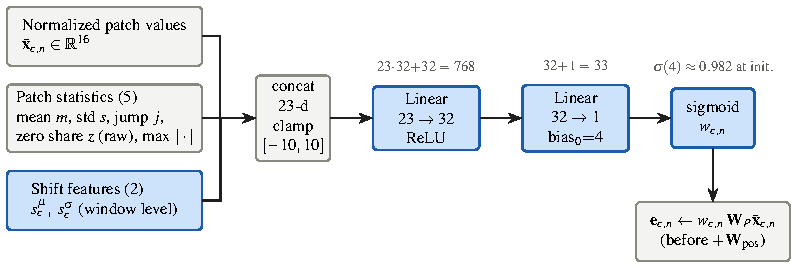
\includegraphics[width=\linewidth]{fig_gate.pdf}
\caption{Reliability gate. Each patch is scored from its 16 normalized values, five patch statistics and the two shift features of its channel. The score multiplies the patch embedding.}
\label{fig:gate}
\end{figure}

\subsection{Shift-Aware Head}
\label{sec:method-shift}

Instance normalization~\eqref{eq:revin} makes the encoder blind to where a window sits relative to the data the model was trained on: a window whose level has moved by two standard deviations looks the same after normalization as an ordinary one. The window statistics are added back at the output~\eqref{eq:head}, but only as an affine correction, so the shape of the forecast cannot depend on them. We compute two shift numbers per channel,
\begin{equation}
s^{\mu}_c=\frac{\mu_c-\bar{\mu}_c}{\bar{\sigma}_c},\qquad s^{\sigma}_c=\frac{\sigma_c}{\bar{\sigma}_c},
\label{eq:shift}
\end{equation}
and append them to the flattened encoder output before the head:
\begin{equation}
\hat{\mathbf{y}}^{N}_c=\mathbf{W}'_H\big[\mathbf{h}_c;\ s^{\mu}_c;\ s^{\sigma}_c\big]+\mathbf{b}_H,\qquad \mathbf{W}'_H\in\R^{H\times(ND+2)}.
\label{eq:shifthead}
\end{equation}
This adds $2H=192$ parameters. The idea is related to the de-stationary attention of Non-stationary Transformers~\cite{nstransformer}, which also reinjects removed statistics, but here they enter only the linear head. The same two numbers feed the gate.

\subsection{Corruption Model}
\label{sec:method-corrupt}

All corruptions act on scaled input windows, so a unit of one corresponds to one training standard deviation. Let $\mathbf{M}$ denote the mask of altered positions, $\odot$ the element-wise product and $\mathcal{B}(p)$ an independent Bernoulli draw per position.

\textit{Missing values (point):} $\mathbf{M}\sim\mathcal{B}(p)$ and $\tilde{\X}=(\mathbf{1}-\mathbf{M})\odot\X$, i.e., each dropped value is replaced by the training mean (zero).

\textit{Missing values (16-step stretch):} a stretch starts at each position with probability $p/16$ and zeroes the next 16 values of that channel, so the expected coverage is close to $p$ and a whole patch length can be lost at once.

\textit{Noise:} $\mathbf{M}\sim\mathcal{B}(p)$ and $\tilde{\X}=\X+\mathbf{M}\odot\bm{\epsilon}$ with $\epsilon_{i,c}\sim\mathcal{N}(0,1)$.

\textit{Anomaly (spike):} $\mathbf{M}\sim\mathcal{B}(p)$ and $\tilde{\X}=\X+\mathbf{M}\odot\mathbf{r}\odot\mathbf{a}$ with magnitudes $a_{i,c}\sim\mathcal{U}(3,5)$ and random signs $r_{i,c}\in\{-1,+1\}$.

\textit{Shift:} for each window and channel, $k$ segments of length $\lfloor L/10\rfloor=33$ with random start are transformed as
\begin{equation}
\tilde{x}_{i,c}=\alpha\,x_{i,c}+\beta,\qquad \alpha\sim\mathcal{U}(0.5,2),\quad \beta\sim\mathcal{U}(-2,2),
\label{eq:shiftcorr}
\end{equation}
with independent $(\alpha,\beta)$ per segment. Segments may overlap.

\textit{Mixed:} shift with $k=1$, then noise, spikes and point-wise missing values, each at $p=5\%$. Missing values are applied last so that dropped values stay exactly zero.

The severity levels are $p\in\{1,5,10,15\}\%$ of points for the first four types and $k\in\{1,3,5,10\}$ segments for shift. Fig.~\ref{fig:corr} shows each type on a real test window.

\begin{figure*}[!t]
\centering
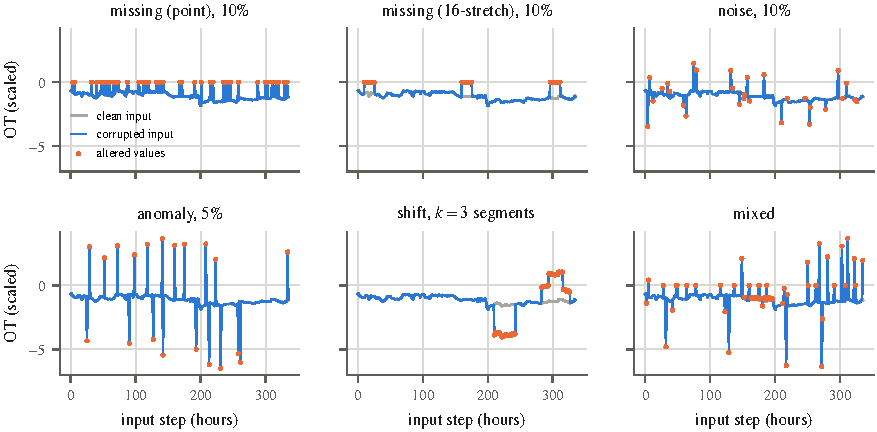
\includegraphics[width=\figwidth]{fig_corruptions.pdf}
\caption{The corruption types applied to one ETTh1 test input window (oil temperature channel, scaled units). Grey: clean input; blue: corrupted input; orange dots: altered values. The panels were drawn with a NumPy port of the project's corruption functions using the same distributions and parameters.}
\label{fig:corr}
\end{figure*}

\subsection{Corruption-Aware Training}
\label{sec:method-cat}

During training each window in a mini-batch is corrupted independently with probability $0.5$ (Fig.~\ref{fig:cat}). For a corrupted window the type is drawn uniformly from \{missing, noise, anomaly, shift\} and the level index uniformly from the four levels; a missing-value corruption is point-wise or stretch-wise with equal probability. The mixed setting is never used for training. The loss~\eqref{eq:mse} is always computed against the clean future, so the network learns to forecast the true continuation from damaged evidence. Because corruption is drawn afresh at every step, the model sees a different damaged copy of each window in every epoch.

\begin{figure}[!t]
\centering
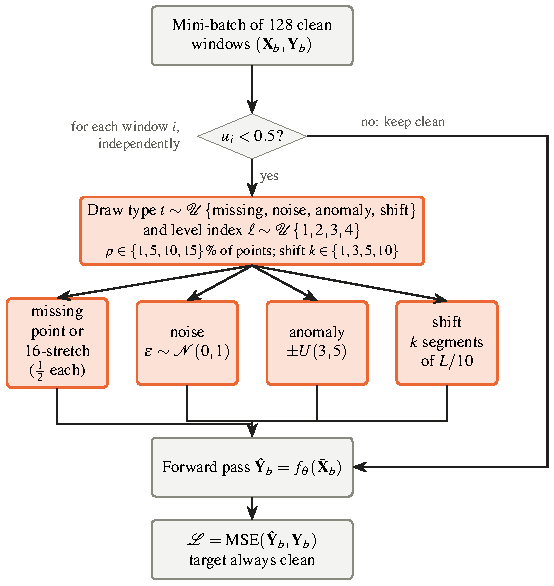
\includegraphics[width=\colfig]{fig_cat.pdf}
\caption{Corruption-aware training. Each window of a mini-batch is corrupted with probability 0.5 using a randomly chosen type and severity. The forecasting loss always uses the clean target.}
\label{fig:cat}
\end{figure}

\subsection{Optimization and Model Selection}
\label{sec:method-opt}

All variants use Adam~\cite{adam} with an initial learning rate $\eta_0=10^{-4}$, batch size 128 and the step decay of the official code (its ``type3'' schedule),
\begin{equation}
\eta_e=\eta_0\cdot0.9^{\max(0,\,e-4)},\qquad e=1,2,\dots
\label{eq:lr}
\end{equation}
Training runs for at most 20 epochs. After each epoch we evaluate the validation MSE on clean windows and on a fixed mixed-corruption copy of the validation set, and keep the checkpoint that minimizes
\begin{equation}
J=\tfrac12\big(\mathrm{MSE}_{\mathrm{val}}^{\mathrm{clean}}+\mathrm{MSE}_{\mathrm{val}}^{\mathrm{mixed}}\big).
\label{eq:select}
\end{equation}
Early stopping uses the same criterion with patience 5. We also keep the checkpoint with the lowest clean validation MSE, which is used only to report the clean reproduction of PatchTST. Algorithm~\ref{alg:train} summarizes the procedure.

\begin{algorithm}[!t]
\caption{Training and selection of one RA-PatchTST variant}
\label{alg:train}
\small
\begin{algorithmic}[1]
\Require training windows $\mathcal{D}_{\mathrm{tr}}$, validation windows $\mathcal{D}_{\mathrm{va}}$, variant flags (gate, shift head, CAT), seed
\State $\tilde{\mathcal{D}}_{\mathrm{va}}\gets$ mixed corruption of $\mathcal{D}_{\mathrm{va}}$ with seed 777
\State initialize $\theta$; gate output bias $c_2\gets4$; $J^\star\gets\infty$; $bad\gets0$
\For{$e=1$ \textbf{to} $20$}
  \State $\eta\gets10^{-4}\cdot0.9^{\max(0,e-4)}$
  \For{each mini-batch $(\X_b,\Y_b)$ of 128 windows, shuffled, last partial batch dropped}
    \If{CAT} \State $\X_b\gets$ corrupt each window with probability 0.5 (random type and level) \EndIf
    \State $\hat{\Y}_b\gets f_\theta(\X_b)$ \Comment{Eqs.~\eqref{eq:revin}--\eqref{eq:shifthead}}
    \State $\theta\gets\mathrm{Adam}\big(\theta,\nabla_\theta\,\mathrm{MSE}(\hat{\Y}_b,\Y_b),\eta\big)$
  \EndFor
  \State $J\gets\frac12\big(\mathrm{MSE}(f_\theta,\mathcal{D}_{\mathrm{va}})+\mathrm{MSE}(f_\theta,\tilde{\mathcal{D}}_{\mathrm{va}})\big)$
  \If{$J<J^\star$} \State $J^\star\gets J$;\ $\theta^\star\gets\theta$;\ $bad\gets0$ \Else \State $bad\gets bad+1$ \EndIf
  \If{$bad\ge5$} \textbf{break} \EndIf
\EndFor
\State \Return $\theta^\star$
\end{algorithmic}
\end{algorithm}

\subsection{Model Variants}
\label{sec:method-variants}

The ablation adds one component at a time (Table~\ref{tab:variants}). A0 is the PatchTST baseline. A1 adds corruption-aware training only, so it isolates the effect of the training data. A2 and A3 add the shift-aware head and the gate respectively on top of A1, and A4 is the full RA-PatchTST. Two further variants are defined in the code, A5 (A4 without corruption-aware training) and A6 (A4 with a gate that does not see the shift features), but they were not run and no result is reported for them.

\begin{table}[!t]
\centering
\caption{Model Variants of the Ablation}
\label{tab:variants}
\footnotesize
\colfit{%
\begin{tabular}{@{}lcccrl@{}}
\toprule
Variant & CAT & Shift head & Gate & Params & Status \\
\midrule
A0 PatchTST & -- & -- & -- & 81,728 & run, 2 seeds \\
A1 & \checkmark & -- & -- & 81,728 & run, 2 seeds \\
A2 & \checkmark & \checkmark & -- & 81,920 & run, 2 seeds \\
A3 & \checkmark & -- & \checkmark & 82,529 & run, 2 seeds \\
A4 RA-PatchTST & \checkmark & \checkmark & \checkmark & 82,721 & run, 2 seeds \\
A5 & -- & \checkmark & \checkmark & 82,721 & defined, not run \\
A6 & \checkmark & \checkmark & \checkmark$^{\dagger}$ & 82,657 & defined, not run \\
\bottomrule
\multicolumn{6}{@{}p{0.95\linewidth}@{}}{\scriptsize CAT: corruption-aware training. $^{\dagger}$Gate without the two shift features (21 inputs instead of 23).}
\end{tabular}}
\end{table}

\subsection{Complexity}
\label{sec:method-complexity}

For a batch of $B$ windows, self-attention costs $O(B\,C\,N^2 D)$ per layer and the feed-forward network $O(B\,C\,N\,D\,d_{ff})$. The gate adds $O(B\,C\,N\cdot(23\cdot32+32))$ operations, roughly the cost of one extra feed-forward layer of width 32 on the patch tokens, and the shift head adds $O(B\,C\,H)$. Neither changes the asymptotic cost. The parameter count of the backbone breaks down as follows: patch embedding 272, position encoding 672, three encoder layers of 5,392 each (attention projections 1,088, two BatchNorms 64, feed-forward 4,240) and the head 64,608, for 81,728 in total. The head dominates, and the gate and shift head together add 993 parameters (1.2\%).

\section{System Architecture}
\label{sec:arch}

The system has two parts: a Python research pipeline that prepares the data, corrupts inputs, trains and evaluates the variants and produces the reports, and a self-contained browser application that runs the trained baseline and RA-PatchTST side by side. Fig.~\ref{fig:pipeline} shows how data move through the pipeline.

\begin{figure*}[!t]
\centering
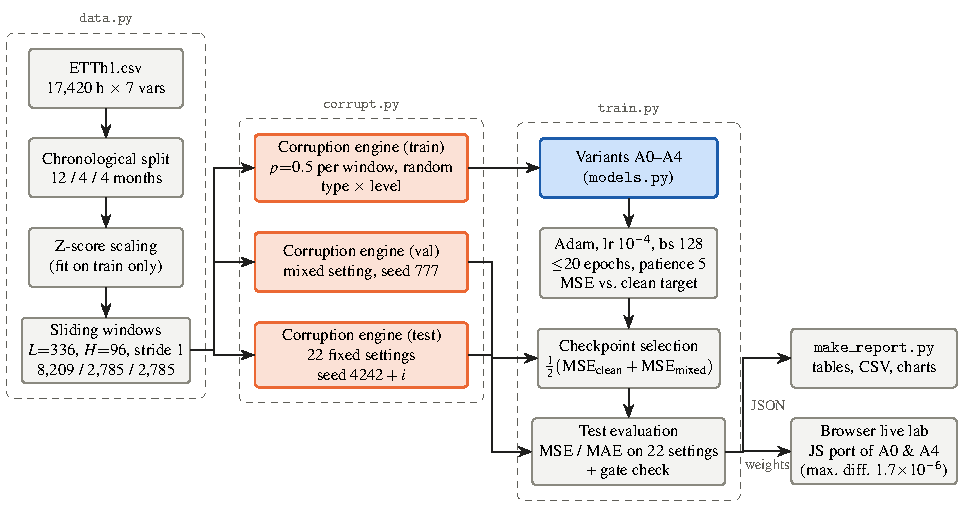
\includegraphics[width=0.92\textwidth]{fig_pipeline.pdf}
\caption{End-to-end pipeline. The same corruption engine produces random corruptions during training, one fixed mixed corruption of the validation set for model selection, and 22 fixed, seeded corruptions of the test set. Results are written as JSON files from which every table and chart is generated; the weights of A0 and A4 are exported to the browser application.}
\label{fig:pipeline}
\end{figure*}

\subsection{Module Design}

The code base consists of five Python modules with narrow interfaces (Table~\ref{tab:modules}). The data module returns tensors only and knows nothing about corruption. The corruption engine is a set of pure functions that take a scaled batch and a seeded random generator and return the corrupted batch together with the mask of altered positions; the same functions serve training, validation and testing, so the corruption seen in evaluation is guaranteed to be the one described in Section~\ref{sec:method-corrupt}. The model module defines a single class whose constructor flags switch the gate and the shift head on or off, and a table that maps each variant name to its flags. The training module owns optimization, selection, evaluation and the gate check, and writes one JSON file per (variant, seed). The report module reads only those JSON files.

\begin{table*}[!t]
\centering
\caption{Software Modules, Responsibilities and Interfaces}
\label{tab:modules}
\footnotesize
\renewcommand{\arraystretch}{1.15}
\begin{tabular}{@{}p{0.14\textwidth}p{0.42\textwidth}p{0.38\textwidth}@{}}
\toprule
Module & Responsibility & Input $\rightarrow$ output \\
\midrule
\texttt{data.py} & Chronological split, train-only scaling, sliding windows, training statistics & CSV file $\rightarrow$ train/val/test tensors, $\bar{\mu}_c,\bar{\sigma}_c$ \\
\texttt{corrupt.py} & Five corruption types, 22 test settings, training-time corruption, patch masks & window batch, seed $\rightarrow$ corrupted batch, mask \\
\texttt{models.py} & PatchTST backbone, reliability gate, shift head; variants A0 to A6 & window batch $\rightarrow$ forecast (and gate weights) \\
\texttt{train.py} & Training loop, checkpoint selection, resumable per-epoch checkpoints, test sweep, gate check & variant, seed $\rightarrow$ result JSON \\
\texttt{make\_report.py} & Aggregation over seeds, tables and charts & result JSON files $\rightarrow$ Markdown, CSV, PNG \\
Live lab (HTML) & JavaScript forward pass of A0 and A4 with embedded weights and test windows & user edits $\rightarrow$ two forecasts, errors, gate weights \\
\bottomrule
\end{tabular}
\end{table*}

\subsection{Tensor Flow Through the Model}

Table~\ref{tab:shapes} traces the shape of the data through one forward pass for a batch of $B$ windows. Channel independence is implemented by folding the channel axis into the batch axis before the encoder and unfolding it before the head; the gate and shift features are computed per channel before folding.

\begin{table}[!t]
\centering
\caption{Tensor Shapes in One Forward Pass}
\label{tab:shapes}
\footnotesize
\colfit{%
\begin{tabular}{@{}ll@{}}
\toprule
Stage & Shape \\
\midrule
Input window $\X$ & $(B,\ 336,\ 7)$ \\
Window statistics $\mu,\sigma$; shift numbers $s^{\mu},s^{\sigma}$ & $(B,\ 7)$ each \\
Patches $\mathbf{p}$ & $(B,\ 7,\ 42,\ 16)$ \\
Gate input $\mathbf{g}$ / gate weights $w$ & $(B,\ 7,\ 42,\ 23)$ / $(B,\ 7,\ 42)$ \\
Embeddings $\mathbf{u}^{(0)}$ (channels folded) & $(7B,\ 42,\ 16)$ \\
Encoder output & $(7B,\ 42,\ 16)$ \\
Head input $[\mathbf{h}_c;s^{\mu}_c;s^{\sigma}_c]$ & $(B,\ 7,\ 674)$ \\
Forecast $\hat{\Y}$ & $(B,\ 96,\ 7)$ \\
\bottomrule
\end{tabular}}
\end{table}

\subsection{Evaluation Subsystem}

Evaluation is deterministic by design. Test setting $i$ ($i=0,\dots,21$) is generated once from the clean test windows with generator seed $4242+i$, and the validation mixed set with seed 777, so all variants and seeds are scored on identical corrupted inputs. For the gated variants the evaluation also reads the gate weights for seven representative settings and splits them by a patch-level mask: a patch counts as corrupted if any of its 16 values was altered, computed by padding and unfolding the position mask exactly as the input is patched.

\subsection{Interactive Live Laboratory}

The live laboratory is a single HTML file that needs no server or network connection. It contains a JavaScript port of the forward pass of A0 and A4 (seed 2021), their trained weights, and a fixed set of 24 ETTh1 test windows. A user picks a window and a channel, applies damage through presets (missing stretches, noise, spikes, level and scale shifts, mixed) or by dragging individual readings, and sees the true future, both forecasts, the damaged input and the trust that the A4 gate gives each patch. A benchmark button runs both models on all $24\times7=168$ sample series under the current damage settings. A dashboard tab shows the experimental results of Section~\ref{sec:results} and states their limitations. When the page was built, the JavaScript forward pass was compared with PyTorch on sample windows and differed by at most $1.7\times10^{-6}$.

\section{Implementation}
\label{sec:impl}

\subsection{Environment}

The system is written in Python~3 with PyTorch~\cite{pytorch}, NumPy and pandas, and matplotlib for the charts. All experiments ran on a cloud CPU container with two virtual cores (Intel Xeon class, 2.1~GHz). Training used two worker processes with one thread each, running the (variant, seed) jobs in a fixed priority order; the script skips jobs whose result file already exists and saves a checkpoint after every epoch, so an interrupted schedule resumes where it stopped. No GPU was used, and a laptop CPU is sufficient to reproduce every run at roughly 40~s per epoch.

\subsection{Hyperparameters}

Table~\ref{tab:hparams} lists every setting. The backbone values are those of the official PatchTST script for ETTh1. No hyperparameter search was carried out for any variant; all variants share the same settings and training budget, so differences between them are attributable to the components being ablated and to seed variation.

\begin{table}[!t]
\centering
\caption{Hyperparameters (Identical for All Variants)}
\label{tab:hparams}
\footnotesize
\colfit{%
\begin{tabular}{@{}ll@{}}
\toprule
Setting & Value \\
\midrule
Look-back $L$ / horizon $H$ & 336 / 96 \\
Patch length $P$ / stride $S$ / patches $N$ & 16 / 8 / 42 \\
Encoder layers / heads / $D$ / FFN width & 3 / 4 / 16 / 128 \\
Dropout & 0.3 \\
Gate hidden width / output bias init. & 32 / $+4$ \\
Gate input clamp & $[-10,10]$ \\
Optimizer / initial learning rate & Adam / $10^{-4}$ \\
Learning-rate decay & $\times0.9$ per epoch after epoch 4 \\
Batch size & 128 (last partial batch dropped) \\
Max.\ epochs / early-stopping patience & 20 / 5 \\
Corruption probability in training & 0.5 per window \\
Training seeds & 2021, 2022 \\
Validation / test corruption seeds & 777 / $4242+i$ \\
Gate penalty $\lambda$ & 0 (not used) \\
\bottomrule
\end{tabular}}
\end{table}

\subsection{Faithfulness to the Official PatchTST}

The backbone was re-implemented from the official code~\cite{patchtst_code} rather than imported, so that the gate and shift head could be inserted at the exact points shown in Fig.~\ref{fig:arch}. It reproduces instance normalization without affine parameters, end padding, patch length 16 with stride 8, the learnable position encoding initialized uniformly in $[-0.02,0.02]$, post-norm encoder layers with BatchNorm, residual attention scores and GELU, and the flatten-linear head. Three small deviations were made, all documented with the code:
\begin{enumerate}
\item dropout is implemented with a uniform random mask ($\mathbf{x}\odot\mathbb{1}[\mathbf{u}\ge p]/(1-p)$, $\mathbf{u}\sim\mathcal{U}(0,1)$), which is mathematically the same inverted dropout but about twice as fast on the CPU;
\item the gate input is clamped to $[-10,10]$ to keep spikes from saturating the gate MLP;
\item the checkpoint used for corrupted-data results is chosen by the combined criterion~\eqref{eq:select} instead of clean validation loss alone, and the clean-validation checkpoint is kept separately for the reproduction check.
\end{enumerate}
The training budget is also smaller than the official one (20 epochs instead of up to 100), which is discussed with the results.

\subsection{Verification}

Before the experiments, the pipeline was checked with the tests in Table~\ref{tab:tests}. They confirm the split sizes, that scaling uses training statistics only, that corruption is deterministic for a given seed and touches only masked positions, that parameter counts match the design, that the untrained gate starts near one, that saved weights reproduce the stored results, and that the browser port agrees with PyTorch.

\begin{table*}[!t]
\centering
\caption{Verification Tests and Their Outcomes}
\label{tab:tests}
\footnotesize
\renewcommand{\arraystretch}{1.12}
\begin{tabular}{@{}lp{0.19\textwidth}p{0.22\textwidth}p{0.18\textwidth}p{0.24\textwidth}l@{}}
\toprule
ID & Purpose & Input & Expected & Observed & Result \\
\midrule
T1 & Window counts & ETTh1, $L=336$, $H=96$ & 8,209 / 2,785 / 2,785 & 8,209 / 2,785 / 2,785 & Pass \\
T2 & Train-only scaling & Training split & Mean 0, std 1 per variable & 0.0 and 1.0 for all 7 variables & Pass \\
T3 & Deterministic corruption & Mixed corruption, seed 4242 twice, then 4243 & Same seed identical; different seed differs & Identical; differs & Pass \\
T4 & Only masked values change & Missing, noise, spike, shift on 128 windows & Unmasked values unchanged & Unchanged for all four; 9.9\% altered at the 10\% level & Pass \\
T5 & Parameter counts & A0, A4, gate & 81,728 / 82,721 / 801 & 81,728 / 82,721 / 801 & Pass \\
T6 & Untrained gate near 1 & A4, untrained, 32 windows & $\approx0.98$ & 0.984 & Pass \\
T7 & Saved weights reproduce results & A0 and A4, seed 2021, clean and mixed test MSE & Match result files & 0.3785/0.4491 (A0), 0.3815/0.4276 (A4) & Pass \\
T8 & Browser port matches PyTorch & Sample windows & Max.\ difference $<10^{-5}$ & $1.7\times10^{-6}$ & Pass \\
T9 & Baseline reproduces paper & ETTh1, $H=96$ & Within 2\% of 0.375 & 0.379 ($+1.1\%$) & Pass \\
\bottomrule
\end{tabular}
\end{table*}

\subsection{Reproducibility}

All randomness is seeded. The training seed fixes model initialization, batch order and, through a separate generator offset by 1000, the training-time corruption. Corrupted evaluation sets use their own fixed seeds. The public ETTh1 file is used unchanged. Every number in Section~\ref{sec:results} is computed by script from the per-run JSON files, which also store the per-epoch training history; the tables and figures of this paper were regenerated from those files.

\section{Experimental Setup}
\label{sec:exp}

\subsection{Dataset}

ETTh1 is the hourly subset of the Electricity Transformer Temperature dataset introduced with Informer~\cite{informer} and distributed through the ETDataset repository~\cite{ettdata} and the Time-Series-Library~\cite{tslib_code}. The file covers 1 July 2016 to 26 June 2018 (17,420 hourly records) from one power transformer in China. It has seven variables: six load features (high, middle and low useful and useless load: HUFL, HULL, MUFL, MULL, LUFL, LULL) and the oil temperature OT. We found no missing values, no duplicate timestamps and no gaps in the hourly spacing. The load features contain negative values and large excursions (HUFL ranges from $-22.7$ to $23.6$), which we keep because they are part of the recorded signal. The data contain no personal information.

Following the standard protocol, the first 12 months form the training set, the next four months the validation set and the following four months the test set; the remaining 3,020 hours are not used. Table~\ref{tab:split} gives the periods and window counts, and Fig.~\ref{fig:dataset} shows two of the variables with the split. The test period falls in winter. Its mean oil temperature is 4.85 against 17.13 in the training year, and the standard deviation of HUFL is 7.66 against 5.81, so even the clean test set is shifted relative to training. Because windows are cut with stride 1, neighbouring samples overlap and are not independent.

\begin{table}[!t]
\centering
\caption{Chronological Split of ETTh1}
\label{tab:split}
\footnotesize
\colfit{%
\begin{tabular}{@{}llr@{}}
\toprule
Split & Period (hourly records) & Windows ($L{=}336$, $H{=}96$) \\
\midrule
Train & 2016-07-01 to 2017-06-25 (8,640) & 8,209 \\
Validation & 2017-06-26 to 2017-10-23 (2,880) & 2,785 \\
Test & 2017-10-24 to 2018-02-20 (2,880) & 2,785 \\
\bottomrule
\end{tabular}}
\end{table}

\begin{figure*}[!t]
\centering
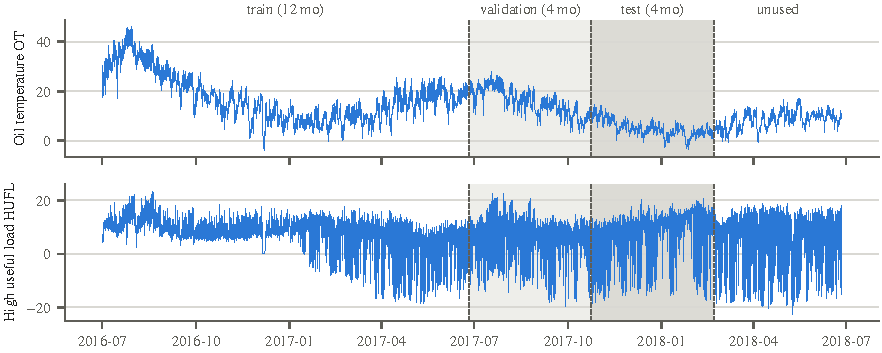
\includegraphics[width=\figwidth]{fig_dataset.pdf}
\caption{Two ETTh1 variables over the full recording with the chronological split. The shaded regions are the validation and test periods; the last 3,020 hours are not used.}
\label{fig:dataset}
\end{figure*}

\subsection{Test Conditions}

Each model is evaluated on 22 versions of the 2,785 test windows (Table~\ref{tab:settings}): the clean inputs, four severity levels for each of the five corruption families, and the mixed setting. Only the input windows are corrupted; the target is the clean future in every case. The mixed setting combines all four training families but at a fixed combination never seen during training.

\begin{table}[!t]
\centering
\caption{The 22 Test Conditions}
\label{tab:settings}
\footnotesize
\renewcommand{\arraystretch}{1.12}
\colfit{%
\begin{tabular}{@{}p{0.28\linewidth}p{0.36\linewidth}p{0.24\linewidth}@{}}
\toprule
Family & Parameters & Levels \\
\midrule
Clean & none & 1 \\
Missing (point) & fraction $p$ of values set to 0 & $p\in\{1,5,10,15\}\%$ \\
Missing (16-stretch) & stretches of 16 zeros, coverage $\approx p$ & $p\in\{1,5,10,15\}\%$ \\
Noise & $+\mathcal{N}(0,1)$ on fraction $p$ & $p\in\{1,5,10,15\}\%$ \\
Anomaly (spike) & $\pm\,\mathcal{U}(3,5)$ on fraction $p$ & $p\in\{1,5,10,15\}\%$ \\
Shift & $k$ segments of 33 steps, $\alpha\!\sim\!\mathcal{U}(0.5,2)$, $\beta\!\sim\!\mathcal{U}(-2,2)$ & $k\in\{1,3,5,10\}$ \\
Mixed & shift $k{=}1$ + noise, spike, missing at 5\% each & 1 \\
\bottomrule
\end{tabular}}
\end{table}

\subsection{Metrics}

We report the mean squared error and mean absolute error on the scaled data,
\begin{equation}
\begin{gathered}
\mathrm{MSE}=\frac{1}{|\mathcal{T}|HC}\sum_{\mathcal{T}}\sum_{i=1}^{H}\sum_{c=1}^{C}(\hat{y}_{i,c}-y_{i,c})^2,\\
\mathrm{MAE}=\frac{1}{|\mathcal{T}|HC}\sum_{\mathcal{T}}\sum_{i=1}^{H}\sum_{c=1}^{C}|\hat{y}_{i,c}-y_{i,c}|,
\end{gathered}
\label{eq:metrics}
\end{equation}
where $\mathcal{T}$ is the set of test windows; lower is better for both. Scaled units make the numbers comparable with published ETTh1 results. Results are aggregated by family (mean over the four levels) and as the mean over all 21 corrupted conditions. Relative change against a reference variant is $\Delta=100\,(\mathrm{MSE}_{v}/\mathrm{MSE}_{\mathrm{ref}}-1)\%$, computed from seed-averaged values, so negative values mean improvement. Gate behaviour is measured as the mean gate weight over corrupted and over clean patches.

\subsection{Statistical Treatment}

Each variant was trained with two seeds (2021 and 2022). We report means with the sample standard deviation over the two seeds, the per-seed values for the headline numbers, and a paired comparison of each variant with A1 in each seed. Two seeds and overlapping test windows do not support formal significance tests or confidence intervals, so we do not report any; the standard deviations should be read as indicating the spread between two runs, nothing more.

\subsection{Baselines}

The baseline is our PatchTST re-implementation (A0). No other published method was re-run under this protocol, so the paper makes no claim about RA-PatchTST relative to DLinear, iTransformer, SEER, TFPS, APT or any other model.

\section{Results and Discussion}
\label{sec:results}

All results are on the ETTh1 test split (2,785 windows, horizon 96, scaled units) and are means over two seeds unless stated otherwise. Table~\ref{tab:headline} gives the headline comparison between the baseline and the full model with the per-seed values; Tables~\ref{tab:groups-mse} to~\ref{tab:delta-a1} break the results down by corruption family and variant, and Appendix~\ref{app:full} lists every condition.

\begin{table}[!t]
\centering
\caption{Headline Results: PatchTST (A0) Versus RA-PatchTST (A4)}
\label{tab:headline}
\footnotesize
\colfit{%
\begin{tabular}{@{}llccl@{}}
\toprule
Model & Test condition & MSE & MAE & Per-seed MSE \\
\midrule
\tabin{tab_headline}
\bottomrule
\end{tabular}}
\end{table}

\subsection{Clean-Data Reproduction (O1)}

Table~\ref{tab:repro} reports the clean test error of each variant with the checkpoint chosen on clean validation loss, which is how PatchTST is usually evaluated. The baseline A0 reaches MSE 0.3791 and MAE 0.4008, against 0.375 and 0.399 published for PatchTST/42~\cite{patchtst}, a gap of 1.1\% in MSE and 0.5\% in MAE, which meets the 2\% target. The remaining gap is plausibly due to the shorter training budget: seed 2021 of A0 reached its best validation score in the last allowed epoch (Table~\ref{tab:cost}), so it had not finished improving. In every run the two checkpoint rules happened to select the same epoch, so the clean numbers in Tables~\ref{tab:headline} and~\ref{tab:repro} coincide.

\begin{table}[!t]
\centering
\caption{Clean Test Error With the Clean-Validation Checkpoint, Against the Published PatchTST/42 Result (MSE 0.375, MAE 0.399)}
\label{tab:repro}
\footnotesize
\colfit{%
\begin{tabular}{@{}lcccc@{}}
\toprule
Variant & MSE & MAE & $\Delta$MSE vs.\ paper & $\Delta$MAE vs.\ paper \\
\midrule
\tabin{tab_repro}
\bottomrule
\end{tabular}}
\end{table}

\subsection{How Much Does Corruption Hurt PatchTST? (RQ1)}

The baseline degrades very unevenly across corruption families (first column of Table~\ref{tab:groups-mse}, Fig.~\ref{fig:groups}). Point-wise missing values, 16-step stretches and noise raise its MSE by only 0.005 to 0.013 on average, and even at 15\% the worst of them costs 7\% (missing stretches, 0.406). Spikes raise the mean MSE to 0.458 ($+20.9\%$) and segment-level shift to 0.520 ($+37.1\%$); at ten shifted segments the MSE reaches 0.712, 88\% above the clean value. Averaged over all 21 corrupted conditions the baseline loses 13.3\%.

Instance normalization explains most of this pattern. A zero in a scaled series is the training mean, which instance normalization turns into a moderate value, and Gaussian noise of one standard deviation on a few percent of the points barely changes the window statistics. A spike of 3 to 5 standard deviations, on the other hand, inflates $\sigma_c$ in~\eqref{eq:revin}, which compresses every other value of the window after normalization and then stretches the forecast when the statistics are restored. A shifted segment moves both $\mu_c$ and $\sigma_c$ and changes the local shape that the patches encode. In both cases the damage spreads, through the window statistics, to every patch of the window.

\begin{table*}[!t]
\centering
\caption{Test MSE by Corruption Family (Mean $\pm$ Standard Deviation Over Two Seeds; Best in Bold)}
\label{tab:groups-mse}
\footnotesize
\begin{tabular}{@{}lccccc@{}}
\toprule
Test condition & A0 PatchTST & A1 +CAT & A2 +CAT+shift head & A3 +CAT+gate & A4 RA-PatchTST \\
\midrule
\tabin{tab_groups_mse}
\bottomrule
\end{tabular}
\end{table*}

\begin{table*}[!t]
\centering
\caption{Test MAE by Corruption Family (Mean $\pm$ Standard Deviation Over Two Seeds; Best in Bold)}
\label{tab:groups-mae}
\footnotesize
\begin{tabular}{@{}lccccc@{}}
\toprule
Test condition & A0 PatchTST & A1 +CAT & A2 +CAT+shift head & A3 +CAT+gate & A4 RA-PatchTST \\
\midrule
\tabin{tab_groups_mae}
\bottomrule
\end{tabular}
\end{table*}

\begin{figure*}[!t]
\centering
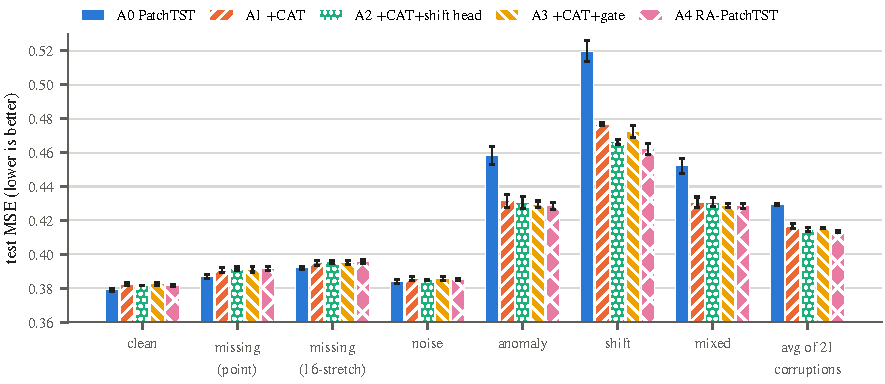
\includegraphics[width=\figwidth]{fig_mse_groups.pdf}
\caption{Test MSE by corruption family for the five variants (mean over two seeds; error bars show the standard deviation between seeds). Note that the vertical axis starts at 0.36.}
\label{fig:groups}
\end{figure*}

\subsection{Effect of RA-PatchTST (RQ2, H1)}

The full model lowers the average MSE over the 21 corrupted conditions from 0.429 to 0.413, a reduction of 3.7\% (Table~\ref{tab:delta-a0}). The reduction is 11.0\% under shift, 6.5\% under spikes and 5.2\% in the mixed setting, and the same ordering holds for MAE (Table~\ref{tab:groups-mae}). The price is a small loss elsewhere: $+0.7\%$ on clean inputs, $+1.3\%$ under point-wise missing values, $+0.9\%$ under missing stretches and $+0.2\%$ under noise. A4 beats A0 in 10 of the 21 corrupted conditions: all four spike levels, all four shift levels, the mixed setting and noise at 15\%. It is worse in the remaining eleven, all of them missing-value or low-level noise conditions where the baseline was already close to its clean error.

The improvement grows with severity (Fig.~\ref{fig:severity}). At one shifted segment A4 is 1.6\% better than A0, at ten segments 20.1\% better (0.569 against 0.712). For spikes the gain rises from 0.6\% at 1\% of points to 11.0\% at 15\%. Fig.~\ref{fig:heatmap} shows the same effect as degradation relative to each model's own clean error: A0 loses 88\% at the worst condition, A4 49\%, and averaged over the 21 conditions A0 loses 13.3\% and A4 8.3\%. For missing values the curves of the three models run nearly parallel, with A0 slightly below.

Against the success criteria of Section~\ref{sec:problem}, A4 lowers the average corrupted MSE in both seeds (0.4132 and 0.4137 against 0.4289 and 0.4298), raises clean MSE by 0.7\% (below the 2\% limit) and adds 1.2\% parameters (below 5\%). H1 is therefore supported on this dataset, with the qualification that the gain is concentrated in two corruption families.

\begin{table}[!t]
\centering
\caption{Change in Test MSE Relative to A0 (Negative Means Better)}
\label{tab:delta-a0}
\footnotesize
\colfit{%
\begin{tabular}{@{}lcccc@{}}
\toprule
Test condition & A1 & A2 & A3 & A4 \\
\midrule
\tabin{tab_delta_a0}
\bottomrule
\end{tabular}}
\end{table}

\begin{figure*}[!t]
\centering
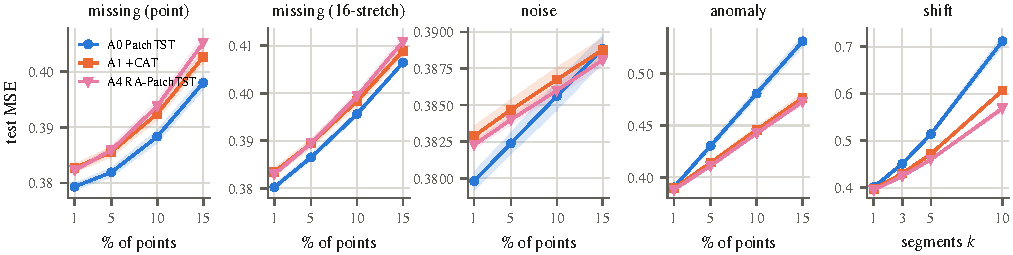
\includegraphics[width=\figwidth]{fig_severity.pdf}
\caption{Test MSE against corruption severity for A0, A1 and A4. Lines are seed means; the shaded bands span the two seeds. Note the different vertical scales.}
\label{fig:severity}
\end{figure*}

\begin{figure*}[!t]
\centering
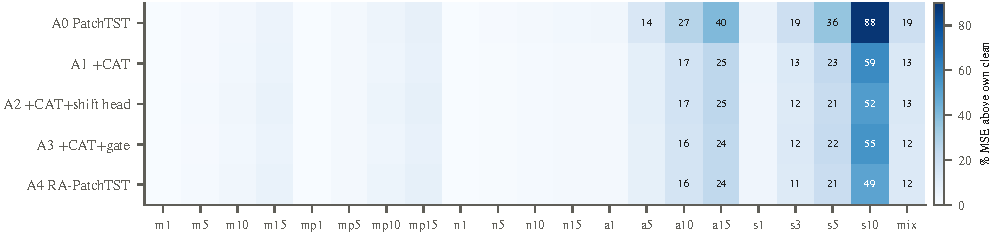
\includegraphics[width=\figwidth]{fig_heatmap.pdf}
\caption{Degradation of each variant relative to its own clean error, $100(\mathrm{MSE}_{\mathrm{cond}}/\mathrm{MSE}_{\mathrm{clean}}-1)$, for the 21 corrupted conditions (m: missing point, mp: missing 16-stretch, n: noise, a: anomaly, s: shift; numbers give the percentage level or the number of shifted segments). Cells of 10\% or more are labelled.}
\label{fig:heatmap}
\end{figure*}

\subsection{Ablation: Where Does the Gain Come From?}

Training on corrupted inputs alone (A1) already gives $-3.0\%$ of the $-3.7\%$ average reduction, that is, about four fifths of the total (Table~\ref{tab:delta-a0}, Fig.~\ref{fig:ablation}). Measured against A1 (Table~\ref{tab:delta-a1}), the shift-aware head (A2) adds $-0.5\%$ on average and $-2.2\%$ under shift, the gate (A3) adds $-0.3\%$ and $-0.9\%$, and the two together (A4) add $-0.8\%$ and $-3.0\%$. The effects of the two components add up almost exactly, which suggests that they address different parts of the problem: the head corrects the level and scale of the forecast, while the gate changes which patches the encoder relies on.

The shift-aware head is the more useful of the two architectural additions, as the analysis of RQ1 would predict: under shift the model needs the window level and scale that instance normalization removes, and the head gives them back. A2 and A4 also reach lower validation errors than A1 and A3 on both the clean and the mixed validation sets (Fig.~\ref{fig:learning}), which points to a benefit that is not limited to the test period.

\begin{table}[!t]
\centering
\caption{Change in Test MSE Relative to A1 (Corruption-Aware Training Only)}
\label{tab:delta-a1}
\footnotesize
\colfit{%
\begin{tabular}{@{}lccc@{}}
\toprule
Test condition & A2 & A3 & A4 \\
\midrule
\tabin{tab_delta_a1}
\bottomrule
\end{tabular}}
\end{table}

\begin{figure}[!t]
\centering
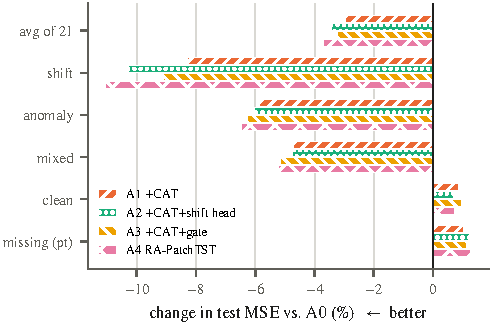
\includegraphics[width=\colfig]{fig_ablation.pdf}
\caption{Change in test MSE relative to A0 for each variant and selected condition groups. Bars to the left of zero are improvements.}
\label{fig:ablation}
\end{figure}

\subsection{Are the Differences Consistent Across Seeds?}

Table~\ref{tab:paired} compares each variant with A1 seed by seed on the average of the 21 corrupted conditions. All three variants improve on A1 in both seeds, and A4 does so by 0.0025 and 0.0039. These differences are small, of the same order as the gap between the two seeds of A1 (0.0020), and with two seeds no significance can be claimed. The comparison with A0 is on firmer ground: the difference between A0 and A4 (0.016) is about 18 times the seed spread of A0 (0.0009) and 32 times that of A4 (0.0005).

\begin{table}[!t]
\centering
\caption{Paired Per-Seed Comparison With A1 on the Average of the 21 Corrupted Conditions}
\label{tab:paired}
\footnotesize
\colfit{%
\begin{tabular}{@{}lcccl@{}}
\toprule
Variant & Seeds & Mean $\Delta$MSE & Seeds better & Per-seed $\Delta$MSE \\
\midrule
\tabin{tab_paired}
\bottomrule
\end{tabular}}
\end{table}

\subsection{Does the Gate Detect Corrupted Patches? (H2)}

Table~\ref{tab:gate} and Fig.~\ref{fig:gate-w} compare the mean gate weight on corrupted and clean patches for seven representative conditions. The gate does react to spikes: in A4 a patch containing a spike receives 0.939 on average, against 0.964 for clean patches in the same windows, and in A3 the gap is wider (0.926 against 0.963). Smaller gaps appear for shift ($-0.017$) and noise ($-0.007$). For missing values, which the zero-share feature was meant to expose, the gate hardly separates damaged from clean patches (a gap of 0.002 to 0.004).

All weights lie between 0.92 and 0.97, so the gate never comes close to switching a patch off; it behaves more like a mild global rescaling with a small extra discount on suspicious patches than like a filter. The gap is also largest for A3, where the gate is the only architectural addition, which suggests that in A4 the shift head takes over part of the work the gate would otherwise do. H2 is supported only weakly, and only for spikes. We therefore do not attribute the robustness of RA-PatchTST mainly to the gate.

\begin{table*}[!t]
\centering
\caption{Mean Gate Weight on Corrupted and Clean Patches (1.0: Fully Trusted). A Patch Counts as Corrupted if Any of Its 16 Values Was Altered}
\label{tab:gate}
\footnotesize
\begin{tabular}{@{}lccccccc@{}}
\toprule
 & & \multicolumn{3}{c}{A3 (+CAT+gate)} & \multicolumn{3}{c}{A4 (RA-PatchTST)} \\
\cmidrule(lr){3-5}\cmidrule(l){6-8}
Condition & Share corrupted & Corrupted & Clean & Gap & Corrupted & Clean & Gap \\
\midrule
\tabin{tab_gate}
\bottomrule
\end{tabular}
\end{table*}

\begin{figure*}[!t]
\centering
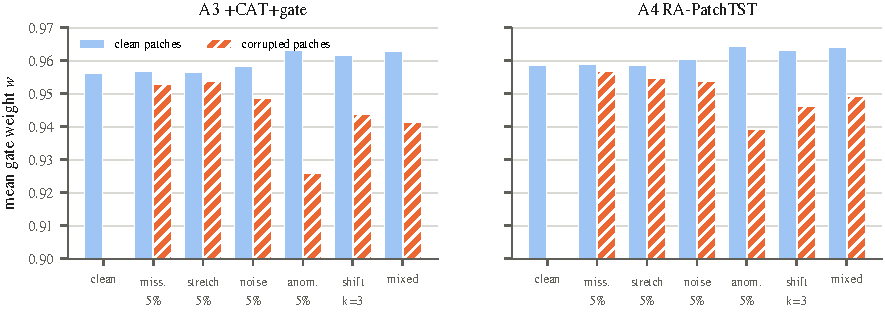
\includegraphics[width=\figwidth]{fig_gate_weights.pdf}
\caption{Mean gate weight on clean and corrupted patches for A3 and A4 (mean over two seeds). The vertical axis spans 0.90 to 0.97: every weight is close to one, and a clear gap appears only for spikes.}
\label{fig:gate-w}
\end{figure*}

\subsection{Training Dynamics}

Fig.~\ref{fig:learning} shows the validation curves. All runs used the full 20 epochs, and the selected checkpoints come from epochs 17 to 20 (Table~\ref{tab:cost}), so none of the models had clearly converged; the official schedule allows up to 100 epochs. On clean validation data A0 ends with the lowest error, as expected for the only model trained on clean data alone. On the mixed validation set the order reverses: at the selected epochs A4 reaches 0.729 to 0.734 and A0 0.761 to 0.765. In every variant the validation MSE is much higher than the test MSE (about 0.68 against 0.38 on clean data), so the two periods differ in difficulty and selection on the validation period transfers to the test period only approximately. Corruption-aware variants also end with higher training loss (0.383 to 0.388 against 0.357 to 0.358 for A0), because half of their training windows are corrupted.

\begin{figure*}[!t]
\centering
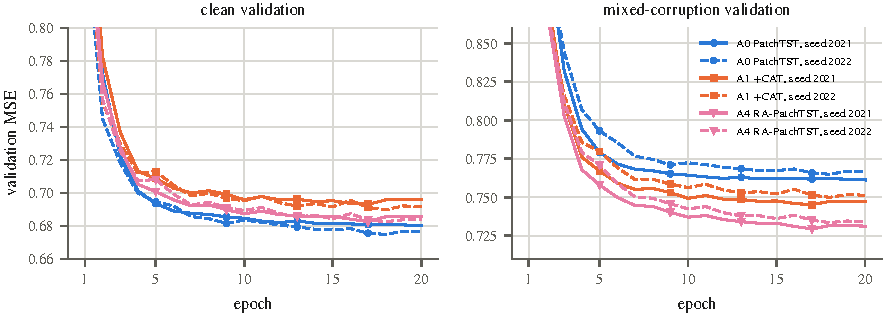
\includegraphics[width=\figwidth]{fig_learning.pdf}
\caption{Validation MSE per epoch for A0, A1 and A4 on clean (left) and mixed-corruption (right) validation windows. Solid lines: seed 2021; dashed lines: seed 2022.}
\label{fig:learning}
\end{figure*}

\subsection{Computational Cost}

Table~\ref{tab:cost} lists the cost of each variant. RA-PatchTST has 993 more parameters than PatchTST (1.2\%), of which 801 are in the gate and 192 in the head. Training time per epoch on one CPU thread rises from 37.0~s to 41.2~s ($+11\%$); 2.0~s of the increase comes from generating corruptions (A1 against A0), 2.0~s from the gate (A3 against A1) and under 1~s from the shift head (A2 against A1). Inference on the 2,785 test windows takes 4.2 to 5.5~s for all variants, and the differences between variants lie within the timing noise of a shared CPU.

\begin{table}[!t]
\centering
\caption{Model Size and Cost (Training Time on One CPU Thread; Inference Over 2,785 Test Windows)}
\label{tab:cost}
\footnotesize
\colfit{%
\begin{tabular}{@{}lrrrccc@{}}
\toprule
Variant & Params & $\Delta$ & Gate & s/epoch & Infer.\ (s) & Sel.\ epoch \\
\midrule
\tabin{tab_cost}
\bottomrule
\multicolumn{7}{@{}l@{}}{\scriptsize Sel.\ epoch: epoch of the selected checkpoint for seeds 2021/2022 (max.\ 20).}
\end{tabular}}
\end{table}

\subsection{Interactive Demonstration}

On the fixed set of 24 test windows $\times$ 7 channels in the live laboratory, with the mixed damage preset, the browser models (seed 2021) give MSE 0.433 for PatchTST and 0.426 for RA-PatchTST ($-1.5\%$), and RA-PatchTST is better on 112 of the 168 series. This is a small demonstration set and not part of the evaluation, but it agrees in direction with the test results.

\subsection{Discussion}

\subsubsection{Interpretation}
The baseline reproduces PatchTST closely and loses accuracy mainly under spikes and shift, in line with the concerns raised about window-local normalization~\cite{fan,apt,revinrole} and patch-level shift~\cite{tfps}. RA-PatchTST reduces these losses, and most of the reduction is due to the training data: a PatchTST that simply sees corrupted windows during training (A1) recovers about 80\% of the gain. The architectural additions help, mostly under shift, and the more effective of them is the simplest one, two numbers appended to the head. The gate learns to discount spikes a little but does not detect missing values.

\subsubsection{Why missing values get slightly worse}
All corruption-aware variants are 0.7 to 1.3\% worse than A0 under missing values and on clean data. Two causes are plausible. First, capacity and training signal are shared: the model spends part of both on spikes and shift, the most damaging families, at a small cost on the mild ones. Second, the zero-filling corruption is easy for the baseline to absorb (a zero is the training mean), so there is little to gain and some precision to lose. The weak response of the gate to missing values may also have a simple cause: the zero-share feature in~\eqref{eq:gatein} is one of 23 inputs, and nothing in the loss rewards the gate for using it.

\subsubsection{Practical significance}
The extra cost is small: 993 parameters, about 11\% more training time and no measurable inference overhead. For data that are mostly clean and complete, RA-PatchTST brings almost no benefit and a slight loss of accuracy. For sensors that are prone to spikes, recalibration jumps or regime changes, the reduction of up to 20\% at high shift severity is a meaningful gain. The model is a research prototype and has not been validated in operation.

\subsubsection{Limitations and threats to validity}
\label{sec:limitations}
The evidence is narrow. Only one dataset (ETTh1), one horizon (96) and one look-back (336) were tested, with two seeds and a 20-epoch budget, and no hyperparameters were tuned. No other published method was re-run, so nothing is claimed relative to SEER~\cite{seer}, TFPS~\cite{tfps}, APT~\cite{apt} or DLinear~\cite{dlinear}. The test corruptions come from the same families that were used in training (only their combination in the mixed setting is new), so the results show robustness to known corruption types, not to unseen ones. The corruptions are synthetic and may differ from real sensor faults. Test windows overlap, so naive confidence intervals would be too narrow. The differences between A2, A3, A4 and A1 are of the same order as the seed variation. Variants A5 and A6 and the gate penalty were not run, so we cannot say how the gate behaves without corruption-aware training or without the shift features. Error analysis by channel or by horizon step was not carried out.

\section{Future Scope}
\label{sec:future}

The limitations above point directly to the next steps, which we order from the most to the least immediate.

\subsubsection{Complete the ablation and strengthen the statistics}
Run at least five seeds per variant, complete A5 (no corruption-aware training) and A6 (gate without shift features), and test the gate penalty $\lambda$. Replace the two-seed standard deviations with confidence intervals from a moving-block bootstrap over test windows~\cite{kunsch}, which respects the overlap between neighbouring windows.

\subsubsection{Broaden the benchmark}
Repeat the protocol on ETTm1, Weather and Electricity and at horizons 192, 336 and 720, with the full training budget of the official code. Re-run DLinear~\cite{dlinear}, iTransformer~\cite{itransformer}, SEER~\cite{seer}, TFPS~\cite{tfps} and APT~\cite{apt} under the same corruption protocol so that the comparison no longer rests on a single baseline.

\subsubsection{Test generalization to unseen damage}
Hold corruption families out of training (for example, train without shift and test with it), add corruption types not modelled here such as stuck-at values, drift ramps and quantization, and evaluate on series with real logged sensor faults rather than synthetic ones.

\subsubsection{Improve the gate}
Give the gate an explicit missing-value mask where the data pipeline can supply one, add a weak auxiliary loss on synthetic corruptions that teaches it where damage is (the corruption engine already produces the mask), and let it act on the attention scores as well as the embeddings. The current result, a gate that stays near one, suggests that the forecasting loss alone gives it too little reason to discriminate.

\subsubsection{Extend the shift signal}
The two shift numbers proved the most useful addition. Richer global descriptors, such as frequency-domain statistics in the spirit of FAN~\cite{fan} or timestamp prototypes as in APT~\cite{apt}, could be passed to the head in the same cheap way, and the effect on clean accuracy should be checked across datasets.

\subsubsection{Towards deployment}
Couple the gate weights with a calibrated uncertainty estimate so that low trust in the input can be reported to an operator, and measure latency on embedded hardware typical of substation monitoring.

\section{Conclusion}
\label{sec:conclusion}

PatchTST gives every input patch the same trust and normalizes away the level and scale of each window, which makes it sensitive to spikes and to shifts in the input. We proposed RA-PatchTST, which adds a patch reliability gate, two shift features for the forecasting head and corruption-aware training, at a cost of 993 parameters, and evaluated it on ETTh1 against a PatchTST re-implementation that reproduces the published clean error to within 1.1\%. Across 21 corrupted test conditions the mean MSE fell from 0.429 to 0.413 ($-3.7\%$), with reductions of 11.0\% under shift, 6.5\% under spikes and 5.2\% under mixed damage, and of 20.1\% at the most severe shift; the clean error rose by 0.7\%.

The ablation qualifies these numbers. Training on corrupted inputs provides about four fifths of the gain. The shift-aware head adds most of the remainder and the gate a little more, and the two effects are additive. The gate discounts spiky patches but does not identify missing values, and its weights stay close to one. The study covers one dataset, one horizon and two seeds, with synthetic corruptions from the training families, so the evidence is preliminary. Within those limits, the results suggest that for patch-based forecasters a large part of the robustness to corrupted inputs can be bought cheaply, through the training data and a global view of shift, and that learning to distrust individual patches needs a stronger signal than the forecasting loss provides.


\section*{Acknowledgment}
The authors thank the Department of Computer Science and Engineering, Ramaiah Institute of Technology, for computing access and guidance. The ETTh1 dataset was released by Zhou \textit{et al.}~\cite{informer} through the ETDataset repository~\cite{ettdata}. The PatchTST re-implementation follows the official code of Nie \textit{et al.}~\cite{patchtst_code}, and the data protocol follows the Time-Series-Library~\cite{tslib_code}.

\bibliographystyle{IEEEtran}
\bibliography{refs}

\appendices
\section{Results for All 22 Test Conditions}
\label{app:full}

Table~\ref{tab:full} gives the test MSE of every variant for every test condition (mean over seeds 2021 and 2022), the MAE of A0 and A4, and the relative change in MSE of A4 against A0. The per-seed values of every run are stored in the result files of the project.

\begin{table*}[!t]
\centering
\caption{Test MSE of All Variants and MAE of A0 and A4 for Every Test Condition (Mean of Two Seeds; Lowest MSE in Bold)}
\label{tab:full}
\footnotesize
\begin{tabular}{@{}lccccccccc@{}}
\toprule
 & \multicolumn{5}{c}{MSE} & \multicolumn{2}{c}{MAE} & \\
\cmidrule(lr){2-6}\cmidrule(lr){7-8}
Condition & A0 & A1 & A2 & A3 & A4 & A0 & A4 & $\Delta$MSE A4 vs.\ A0 \\
\midrule
\tabin{tab_full}
\bottomrule
\end{tabular}
\end{table*}

\section{Data Dictionary}
\label{app:data}

\begin{table}[!h]
\centering
\caption{ETTh1 Variables (Original Units Are Not Stated in the Dataset Documentation)}
\label{tab:dict}
\footnotesize
\colfit{%
\begin{tabular}{@{}llrrrr@{}}
\toprule
Variable & Description & Mean & Std & Min & Max \\
\midrule
HUFL & High useful load & 7.38 & 7.07 & $-22.71$ & 23.64 \\
HULL & High useless load & 2.24 & 2.04 & $-4.76$ & 10.11 \\
MUFL & Middle useful load & 4.30 & 6.83 & $-25.09$ & 17.34 \\
MULL & Middle useless load & 0.88 & 1.81 & $-5.93$ & 7.75 \\
LUFL & Low useful load & 3.07 & 1.16 & $-1.19$ & 8.50 \\
LULL & Low useless load & 0.86 & 0.60 & $-1.37$ & 3.05 \\
OT & Oil temperature (target of interest) & 13.32 & 8.57 & $-4.08$ & 46.01 \\
\bottomrule
\multicolumn{6}{@{}l@{}}{\scriptsize Statistics over all 17,420 records. The \texttt{date} column (hourly timestamps) is dropped before modelling.}
\end{tabular}}
\end{table}

\section{Reproducing the Experiments}
\label{app:repro}

The experiments are reproduced with the commands below, run from the project folder with Python~3, PyTorch, NumPy, pandas and matplotlib installed.

\begin{footnotesize}
\begin{verbatim}
python data.py data_raw/ETTh1.csv
python train.py --variants A0 A1 A2 A3 A4 \
  --seeds 2021 2022 --epochs 20 --patience 5
python make_report.py
\end{verbatim}
\end{footnotesize}

\noindent The first command checks the split shapes, the second trains and evaluates all runs, and the third writes the summary tables and chart.

\noindent \texttt{run\_all.sh} contains the exact two-worker schedule that was used. The figures and tables of this paper are regenerated from the stored result files by \texttt{make\_figures.py} and \texttt{make\_tables.py} in the manuscript repository.


\end{document}
"
\ifdefined\cameraready
  \documentclass[journal]{IEEEtran}
\else
  \documentclass[journal,12pt,onecolumn]{IEEEtran}
\fi

\usepackage{cite}
\usepackage{amsmath,amssymb,amsfonts}
\usepackage{bm}
\usepackage{graphicx}
\usepackage{booktabs}
\usepackage{multirow}
\usepackage{array}
\usepackage{xcolor}
\usepackage{algorithm}
\usepackage{algpseudocode}
\usepackage{textcomp}
\usepackage{url}
\usepackage[hidelinks]{hyperref}
\graphicspath{{figures/}}
\interdisplaylinepenalty=2500

\ifdefined\cameraready
  \newcommand{\figwidth}{\textwidth}
  \newcommand{\colfig}{\columnwidth}
\else
  \newcommand{\figwidth}{0.98\textwidth}
  \newcommand{\colfig}{0.62\textwidth}
\fi

\newcommand{\X}{\mathbf{X}}
\newcommand{\Y}{\mathbf{Y}}
\newcommand{\R}{\mathbb{R}}
\DeclareMathOperator*{\argmin}{arg\,min}

\ifdefined\cameraready
  \newcommand{\colfit}[1]{\resizebox{\columnwidth}{!}{#1}}
\else
  \newcommand{\colfit}[1]{#1}
\fi
\makeatletter\newcommand{\tabin}[1]{\@@input tables/#1.tex }\makeatother
\hyphenation{Patch-TST RA-Patch-TST Trans-former}

\begin{document}

\title{RA-PatchTST: A Reliability-Aware Extension of PatchTST for Multivariate Time-Series Forecasting Under Corrupted Inputs}

\author{Jeevika~N,
        Jnanottam~G~Y,
        and~Mallegowda~M%
\thanks{The authors are with the Department of Computer Science and Engineering, Ramaiah Institute of Technology, MSR Nagar, MSRIT Post, Bengaluru 560054, India. This work was carried out as part of the course Artificial Intelligence and Machine Learning (24CS52), academic year 2026--27.}}

\markboth{RA-PatchTST: Reliability-Aware PatchTST Under Corrupted Inputs}%
{N \MakeLowercase{\textit{et al.}}: RA-PatchTST: Reliability-Aware PatchTST Under Corrupted Inputs}

\maketitle

\begin{abstract}
Patch-based Transformer forecasters such as PatchTST treat every input patch as equally trustworthy, yet sensor series routinely contain missing readings, measurement noise, spikes and shifts in level or scale. This paper presents RA-PatchTST, a reliability-aware extension of PatchTST that adds three small components to the original design: a patch reliability gate (a two-layer perceptron with 801 parameters that scores each patch between 0 and 1 and rescales its embedding), a shift-aware forecasting head that receives the mean and scale of each input window relative to the training statistics, which instance normalization would otherwise discard, and corruption-aware training, in which half of the training windows are corrupted on the fly while the loss is always computed against the clean future. The full model adds 993 parameters (1.2\%) to an 81,728-parameter backbone. We evaluate on the ETTh1 benchmark (17,420 hourly records, seven variables, chronological 12/4/4-month split, look-back 336, horizon 96) using five ablation variants, two random seeds and 22 fixed test conditions: clean data plus 21 seeded corruptions covering point-wise and 16-step missing values, Gaussian noise, spikes, segment-level shift and a mixed setting. Our PatchTST re-implementation reaches a clean test MSE of 0.379 against the published 0.375. RA-PatchTST lowers the mean MSE over the 21 corrupted conditions from 0.429 to 0.413 ($-3.7\%$), with the largest reductions under shift ($-11.0\%$), spikes ($-6.5\%$) and mixed damage ($-5.2\%$), at a cost of $+0.7\%$ on clean data and up to $+1.3\%$ under missing values. The ablation attributes about four fifths of the gain to corruption-aware training; the gate and the shift-aware head add a further $-0.8\%$, concentrated on shift. The gate assigns clearly lower weight to corrupted patches only for spikes. With one dataset, one horizon, two seeds and synthetic corruptions drawn from the training families, these results are preliminary evidence for the approach and do not establish general superiority.
\end{abstract}

\begin{IEEEkeywords}
Time-series forecasting, PatchTST, Transformer, robustness, distribution shift, data corruption, reliability gating, instance normalization, ablation study.
\end{IEEEkeywords}

\section{Introduction}
\label{sec:intro}

\IEEEPARstart{F}{orecasting} the next few days of a multivariate sensor series supports load planning in power networks, scheduling in industrial plants and maintenance of equipment such as power transformers. Deep forecasters for this task have changed quickly over the last five years. Informer~\cite{informer} and its successors Autoformer~\cite{autoformer} and FEDformer~\cite{fedformer} adapted the Transformer~\cite{vaswani} to long sequences. DLinear~\cite{dlinear} then showed that a single linear layer could match or beat these models on the standard long-term benchmarks, and PatchTST~\cite{patchtst} restored the lead of attention-based models by splitting each channel into short overlapping patches, treating each patch as a token and processing channels independently with shared weights. PatchTST is now a common baseline in forecasting studies and in benchmark libraries~\cite{tslib}.

These models are compared on clean benchmarks, while real sensor streams are noisy in several ways: readings go missing when a logger fails, analog channels pick up noise, transient faults produce isolated spikes, and recalibration or a change in operating regime moves a stretch of the series to a different level or scale~\cite{blazquez_anomaly,gama_drift}. In forecasting there are rarely labels that say which inputs are bad~\cite{seer}, so the model has to cope with corrupted inputs without being told where they are.

Two properties of PatchTST make it sensitive to such inputs. First, every patch enters the encoder with the same standing. The attention weights can in principle learn to ignore a damaged patch, but nothing in the architecture or the training signal encourages this. Second, PatchTST normalizes each input window by its own mean and standard deviation (the instance normalization of RevIN~\cite{revin}, without the affine part) and restores those statistics at the output. This helps under slow drift, but it also removes the information that would tell the model that a window sits at an unusual level relative to the training data. Recent analyses argue that window-local statistics cannot capture every kind of shift~\cite{fan,apt,revinrole}.

In our own baseline run, under the segment-level shift corruption described in Section~\ref{sec:exp}, the test MSE of a faithful PatchTST re-implementation on ETTh1 rises from 0.379 on clean inputs to 0.520 on average over four severity levels, and to 0.712 at the highest level. Spikes raise it to 0.458. Missing values and noise, by contrast, cost less than 0.015.

Existing remedies fall into three groups (Section~\ref{sec:lit}). Normalization-based methods such as RevIN~\cite{revin}, Dish-TS~\cite{dishts}, FAN~\cite{fan} and APT~\cite{apt} target distribution shift but do not weigh inputs by quality. Robustness-oriented frameworks such as SEER~\cite{seer}, RobustTSF~\cite{robusttsf} and TameR~\cite{tamer} address noisy or anomalous inputs, but either replace the forecaster with a new architecture, focus on one type of damage, or act only at training time~\cite{tps}. Expert-based and test-time methods such as TFPS~\cite{tfps} and SOLID~\cite{solid} add parameters or per-sample fine-tuning. None of the studies we surveyed offers a small plug-in for PatchTST that scores the reliability of each patch and gives the head a global view of shift within a single forward pass; we make no claim about work outside that set.

This paper studies whether such a plug-in helps, and by how much. We make four contributions.
\begin{enumerate}
\item A reproducible corruption benchmark on ETTh1 with 22 fixed test conditions (clean plus five corruption families at four severity levels and one mixed setting), in which every model sees identical corrupted inputs.
\item RA-PatchTST, which adds to PatchTST a patch reliability gate, two shift features appended to the forecasting head, and corruption-aware training, for 993 extra parameters in total.
\item An ablation over five variants (A0 to A4) and two seeds that separates the contribution of training on corrupted data from that of each architectural component, together with a direct check of whether the gate down-weights corrupted patches.
\item A browser-based live laboratory in which the original and the proposed model run side by side on real ETTh1 test windows that the user can damage interactively.
\end{enumerate}

RA-PatchTST reduces the average corrupted-input MSE by 3.7\% and the shift error by 11.0\%, but most of this gain comes from corruption-aware training, the gate is a weak detector except for spikes, and the model is slightly worse than PatchTST on clean data and under missing values. The PatchTST backbone is a re-implementation of the published design~\cite{patchtst,patchtst_code}; the research contribution lies in the gate, the shift features, their combination with corruption-aware training, and the ablation that measures what each part adds.

The rest of the paper is organized as follows. Section~\ref{sec:lit} reviews related work. Section~\ref{sec:problem} states the problem formally. Section~\ref{sec:method} develops the method, Section~\ref{sec:arch} describes the system architecture and Section~\ref{sec:impl} the implementation. Section~\ref{sec:exp} gives the experimental protocol and Section~\ref{sec:results} the results and their discussion. Sections~\ref{sec:future} and~\ref{sec:conclusion} outline future work and conclude.

\section{Literature Review}
\label{sec:lit}

We carried out a focused narrative review. We searched arXiv, the proceedings of ICLR, ICML, NeurIPS, AAAI and KDD, and the Google Scholar and GitHub pages of the papers found, using the terms \emph{PatchTST}, \emph{patch-based forecasting}, \emph{robust time series forecasting}, \emph{distribution shift}, \emph{instance normalization}, \emph{missing values} and \emph{anomalies}, for the period 2021 to 2026. A study was kept if it builds on or compares with patch-based Transformers, if it addresses corrupted inputs or distribution shift in forecasting, or if it defines the benchmark protocol. Several 2026 entries were preprints at the time of writing. Because the papers use different datasets, horizons and protocols, we do not compare their numbers with ours.

\subsection{From Sequence Transformers to Patch Tokens}

The Transformer~\cite{vaswani} replaced recurrence with self-attention, and Informer~\cite{informer} was among the first to adapt it to long-sequence time-series forecasting, introducing ProbSparse attention and, with it, the ETT datasets that remain a standard benchmark. Autoformer~\cite{autoformer} built series decomposition into the network and replaced point-wise attention with an auto-correlation mechanism, and FEDformer~\cite{fedformer} moved attention into the frequency domain. Zeng \textit{et al.}~\cite{dlinear} then questioned the whole line of work: one-layer linear models with a trend-seasonal split (DLinear) outperformed these Transformers on nine benchmarks, suggesting that point-wise tokens carry too little semantic content for attention to exploit.

PatchTST~\cite{patchtst} answered this by grouping consecutive time steps into patches, in the same spirit as the image patches of the Vision Transformer~\cite{vit}. A look-back of 336 steps cut into patches of 16 with stride 8 gives 42 tokens per channel, which shortens the attention span by a factor of about eight and gives each token local shape information. PatchTST also processes each channel independently with shared weights, and normalizes each input window with its own statistics. The official implementation~\cite{patchtst_code} uses BatchNorm inside the encoder~\cite{batchnorm}, GELU activations~\cite{gelu} and residual attention scores in the style of RealFormer~\cite{realformer}. On ETTh1 with look-back 336 and horizon 96, the supervised PatchTST/42 reports MSE 0.375 and MAE 0.399~\cite{patchtst}.

Later models moved in several directions. TimesNet~\cite{timesnet} reshapes a series into two-dimensional period-by-phase tensors. iTransformer~\cite{itransformer} inverts the token axis and attends across variables instead of time. TimeMixer~\cite{timemixer} mixes seasonal and trend components across scales with MLPs, and xPatch~\cite{xpatch} combines patching with exponential seasonal-trend decomposition in a dual-stream CNN and MLP network. Chronos~\cite{chronos} takes the foundation-model route, scaling and quantizing values into tokens and training a language-model architecture on a large corpus for zero-shot use. The Time-Series-Library survey and benchmark~\cite{tslib,tslib_code} fixes a common protocol for these models, which we follow.

\subsection{Normalization and Distribution Shift}

A forecaster trained on one period and applied to the next faces distribution shift, a problem studied in machine learning under the names dataset shift~\cite{datasetshift} and concept drift~\cite{gama_drift}. RevIN~\cite{revin} handles it by normalizing each input window and restoring its statistics at the output, with optional learnable affine parameters. Non-stationary Transformers~\cite{nstransformer} combine such series stationarization with a de-stationary attention that reinjects the removed statistics into the attention scores, which is the closest prior idea to our shift-aware head. Dish-TS~\cite{dishts} separates the shift within the look-back window from the shift between look-back and horizon. FAN~\cite{fan} argues that mean and variance do not describe non-stationarity in the frequency domain and removes the dominant Fourier components instead. APT~\cite{apt} adds affine prototypes indexed by timestamp because, in its authors' analysis, local mean and variance miss global shift. An analysis of RevIN using PatchTST~\cite{revinrole} finds that some of its parts are redundant or even harmful, and that it does not cover all forms of shift. TS\_Adam~\cite{tsadam} changes the optimizer to cope with drift during training.

Two methods react to shift more actively. TFPS~\cite{tfps} identifies patch-level distribution shift and routes patches to pattern-specific experts in the time and frequency domains. SOLID~\cite{solid} detects context-driven shift and fine-tunes the prediction layer for each test sample on similar training samples, which adds computation at test time just as TFPS adds experts.

\subsection{Robustness to Corrupted Inputs}

Missing values are usually handled by imputation before forecasting, with recurrent models such as BRITS~\cite{brits} or self-attention models such as SAITS~\cite{saits}; anomalies are usually handled by detection~\cite{blazquez_anomaly}. Both add a separate model with its own training and error. Several recent works instead make the forecaster itself tolerant to corruption. RobustTSF~\cite{robusttsf} analyzes forecasting when the training data contain anomalies and proposes a robust training procedure. TameR~\cite{tamer} uses global context to reduce the bias of forecasters toward recent, possibly corrupted, observations and reports gains under noise, missing values and anomalies. SEER~\cite{seer} is the closest work to ours: a Transformer framework with a channel-adaptive module and a learnable patch replacement module that filters low-quality patches, tested under missing values, shifts, anomalies and noise. SEER is a full framework, whereas we ask how much of the benefit a far smaller addition to an unchanged PatchTST can deliver. Temporal Patch Shuffle~\cite{tps} augments training data by shuffling patches and improves the robustness of several model families, PatchTST included, but at test time every patch is still trusted equally.

Our evaluation design borrows from computer vision, where Hendrycks and Dietterich~\cite{hendrycks_corrupt} defined a benchmark of common corruptions at graded severities applied to the test set only. A study of Autoformer, Informer and PatchTST on synthetic signals~\cite{synthbench} similarly compares architectures under controlled noise. Training on corrupted copies of the input is a form of data augmentation, which the survey of Wen \textit{et al.}~\cite{tsaug_survey} reviews for time series.

\subsection{Gating as a Soft Selection Mechanism}

Multiplicative gates with sigmoid outputs are a standard way to let a network decide how much of a signal to pass. LSTM gates~\cite{lstm} control the flow of memory, gated linear units~\cite{glu} modulate convolutional features, and squeeze-and-excitation blocks~\cite{senet} rescale feature channels using a small bottleneck MLP over pooled statistics. Our reliability gate follows the last pattern most closely: a small MLP reads summary statistics of each patch and outputs a scale factor applied to that patch's embedding.

\subsection{Summary and Research Gap}

Table~\ref{tab:lit} summarizes the studies most relevant to this work. Shift-oriented methods change normalization or add experts, but none of them weighs inputs by their quality. The robustness-oriented methods do address corrupted inputs, each in its own way: SEER and TameR with new architectures, RobustTSF with a focus on anomalies, and TPS through augmentation at training time only. The accuracy-oriented models address neither problem. None of them tests how far a few hundred parameters added to an unchanged PatchTST can go, or which of the possible additions helps; Sections~\ref{sec:method} and~\ref{sec:results} take up both questions.

\begin{table*}[!t]
\centering
\caption{Studies Most Relevant to This Work and the Gap Each Leaves Open}
\label{tab:lit}
\footnotesize
\renewcommand{\arraystretch}{1.15}
\begin{tabular}{@{}p{0.17\textwidth}p{0.36\textwidth}p{0.40\textwidth}@{}}
\toprule
Study (venue, year) & Approach & Relevance and limitation for this work \\
\midrule
SEER~\cite{seer} (ICML 2026) & Channel-adaptive module and learnable patch replacement that filters low-quality patches & Closest aim; a full new framework rather than a small add-on to PatchTST \\
APT~\cite{apt} (AAAI 2026) & Affine prototypes indexed by timestamp for shift & Shift only; motivates giving the model global statistics \\
TameR~\cite{tamer} (ICML 2026) & Global context against recent-data bias & Robust to noise, missing values and anomalies; no per-patch reliability score \\
TPS~\cite{tps} (preprint, 2026) & Patch shuffling as training augmentation & Training time only; all patches trusted equally at test time \\
RevIN analysis~\cite{revinrole} (preprint, 2026) & Ablation of RevIN components with PatchTST & Analysis only; supports adding a global view of shift \\
TS\_Adam~\cite{tsadam} (Neurocomputing, 2026) & Optimizer modified for drift & Cannot distinguish reliable from unreliable inputs \\
xPatch~\cite{xpatch} (AAAI 2025) & Dual-stream patching with exponential decomposition & Accuracy-oriented; no input-quality mechanism \\
TFPS~\cite{tfps} (NeurIPS 2025) & Pattern-specific experts for patch-level shift & More parameters; targets shift rather than noise or missing data \\
FAN~\cite{fan} (NeurIPS 2024) & Frequency adaptive normalization & Shift only; does not weigh patches by quality \\
RobustTSF~\cite{robusttsf} (ICLR 2024) & Robust training with anomalous data & Anomalies only; not patch-based \\
SOLID~\cite{solid} (KDD 2024) & Detect context-driven shift, fine-tune per sample & Costly at test time; our gate needs one forward pass \\
iTransformer~\cite{itransformer}, TimeMixer~\cite{timemixer} (ICLR 2024) & Variate tokens; multiscale MLP mixing & Accuracy-oriented baselines \\
Chronos~\cite{chronos} (TMLR 2024) & Pretrained tokenized forecaster & Large pretrained model; not a lightweight fix \\
DLinear~\cite{dlinear} (AAAI 2023) & Linear model with decomposition & Strong simple baseline; no robustness mechanism \\
PatchTST~\cite{patchtst} (ICLR 2023) & Patching, channel independence, instance norm. & Base model; equal trust in all patches, window-local statistics only \\
RevIN~\cite{revin} (ICLR 2022) & Reversible instance normalization & Uses only the window's own mean and variance \\
\bottomrule
\end{tabular}
\end{table*}

\section{Problem Statement}
\label{sec:problem}

\subsection{Forecasting Setting}

Let $\{\mathbf{s}_t\}_{t=1}^{T_{\mathrm{tot}}}$, $\mathbf{s}_t\in\R^{C}$, be a multivariate series with $C$ channels sampled at regular intervals. At time $t$ a forecaster receives the look-back window $\X=[\mathbf{s}_{t-L+1},\dots,\mathbf{s}_t]^{\top}\in\R^{L\times C}$ and predicts the next $H$ steps $\Y=[\mathbf{s}_{t+1},\dots,\mathbf{s}_{t+H}]^{\top}\in\R^{H\times C}$. In this work $C=7$, $L=336$ and $H=96$, so the model reads two weeks of hourly data and forecasts the next four days. A forecaster $f_\theta$ is trained by minimizing the mean squared error
\begin{equation}
\mathcal{L}(\theta)=\mathbb{E}_{(\X,\Y)}\Big[\tfrac{1}{HC}\big\lVert f_\theta(\X)-\Y\big\rVert_F^2\Big].
\label{eq:mse}
\end{equation}

\subsection{Corrupted Inputs}

In deployment the model may receive a corrupted window $\tilde{\X}=\mathcal{C}(\X;\,\kappa,\ell,\xi)$, where $\mathcal{C}$ is a corruption operator of type $\kappa$ (missing values, noise, spike, shift or a mixture), severity $\ell$, and random draw $\xi$. The location of the damage is unknown to the model; we write $\mathbf{M}\in\{0,1\}^{L\times C}$ for the mask of altered positions, which is used only for analysis. The forecast target is never corrupted: the goal is to predict the true future $\Y$ from damaged evidence $\tilde{\X}$. Section~\ref{sec:method-corrupt} defines $\mathcal{C}$ precisely.

\subsection{Problem Definition}

Given a PatchTST forecaster, the problem is to keep the forecast error low when the input is corrupted, with three constraints that make the result usable as a plug-in:
\begin{enumerate}
\item the error on clean inputs should not rise by more than 2\%;
\item the parameter count should not rise by more than 5\%;
\item the model must run in a single forward pass, without a separate imputation or detection model and without test-time adaptation.
\end{enumerate}

\subsection{Research Questions and Hypotheses}

\textit{RQ1:} How much accuracy does a faithful PatchTST lose under controlled input corruption, and which corruption types hurt most?

\textit{RQ2:} Can a reliability gate, a shift-aware head and corruption-aware training reduce that loss, and how much does each contribute?

We test two hypotheses separately.
\begin{itemize}
\item \textbf{H1.} Together, the three components lower the test MSE of PatchTST averaged over the corrupted conditions, while the clean-data MSE changes only slightly.
\item \textbf{H2.} The gate learns to assign lower weight to corrupted patches than to clean patches.
\end{itemize}

\subsection{Objectives and Success Criteria}

Table~\ref{tab:objectives} lists the objectives and how each is measured. The numerical thresholds are practical targets we set for a lightweight add-on, not standards from the literature. The original plan to cover four datasets (ETTh1, ETTm1, Weather, Electricity) and four horizons was reduced to ETTh1 at horizon 96 because all training ran on CPUs; Section~\ref{sec:limitations} returns to this.

\begin{table}[!t]
\centering
\caption{Objectives and Success Criteria}
\label{tab:objectives}
\footnotesize
\renewcommand{\arraystretch}{1.15}
\colfit{%
\begin{tabular}{@{}p{0.06\linewidth}p{0.42\linewidth}p{0.44\linewidth}@{}}
\toprule
ID & Objective & Measure and target \\
\midrule
O1 & Re-implement PatchTST and reproduce its clean ETTh1 result & Test MSE within 2\% of the published 0.375 \\
O2 & Build a seeded corruption benchmark & 22 conditions; identical inputs for all models \\
O3 & Design RA-PatchTST & Parameter increase below 5\% \\
O4 & Compare A0 with variants A1 to A4 & Mean corrupted MSE lower than A0 in every seed; clean MSE increase below 2\% \\
O5 & Check what the gate learns & Mean gate weight on corrupted vs.\ clean patches \\
O6 & Build an interactive demonstration & Browser port agrees with PyTorch within $10^{-5}$ \\
\bottomrule
\end{tabular}}
\end{table}

\section{Proposed Methodology}
\label{sec:method}

RA-PatchTST keeps the PatchTST backbone unchanged and adds three components (Fig.~\ref{fig:arch}). This section first describes data preparation and the backbone, then each addition, the corruption model used for training and testing, and the training objective.

\begin{figure*}[!t]
\centering
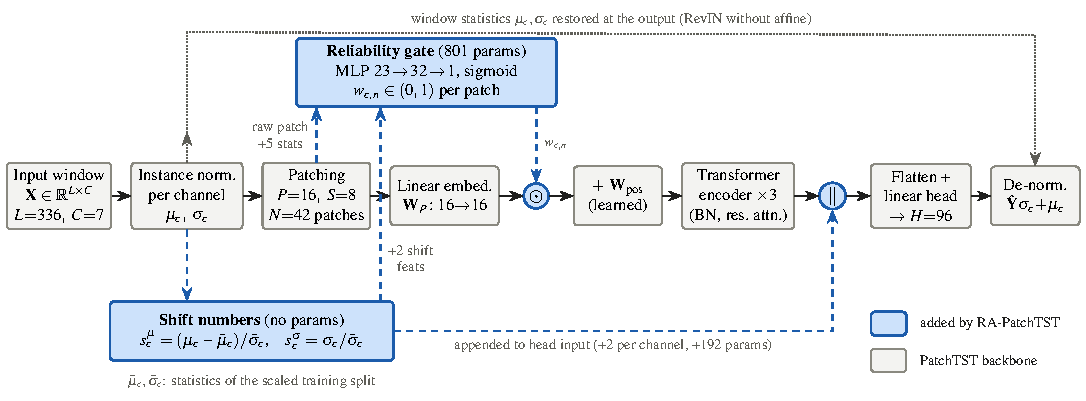
\includegraphics[width=\figwidth]{fig_architecture.pdf}
\caption{RA-PatchTST architecture. Grey blocks are the PatchTST backbone; blue blocks are the components added in this work. The reliability gate scores every patch and rescales its embedding before the position encoding is added; the two shift numbers are computed from the window statistics that instance normalization removes and are appended to the input of the linear head. Corruption-aware training (Fig.~\ref{fig:cat}) changes only the data fed to this network.}
\label{fig:arch}
\end{figure*}

\subsection{Data Preparation}
\label{sec:method-data}

The series is split chronologically into training, validation and test segments (Section~\ref{sec:exp}). A per-channel z-score scaler is fitted on the training segment only and applied to all three,
\begin{equation}
\begin{gathered}
\bar{s}_{t,c}=\frac{s_{t,c}-m_c}{d_c},\qquad m_c=\frac{1}{T_{\mathrm{tr}}}\sum_{t\le T_{\mathrm{tr}}}s_{t,c},\\
d_c^2=\frac{1}{T_{\mathrm{tr}}}\sum_{t\le T_{\mathrm{tr}}}(s_{t,c}-m_c)^2,
\end{gathered}
\label{eq:scale}
\end{equation}
so that no validation or test statistics leak into training. Windows of length $L+H$ are then cut with stride 1. Validation and test windows start $L$ steps before their segment so that the first forecast target lies exactly on the segment border, as in the Time-Series-Library protocol~\cite{tslib_code}. We also store the per-channel mean $\bar{\mu}_c$ and standard deviation $\bar{\sigma}_c$ of the \emph{scaled} training segment, which the shift features use. By construction $\bar{\mu}_c=0$ and $\bar{\sigma}_c=1$ up to rounding; the code keeps them explicit so that the same model can be used with other scalers.

\subsection{PatchTST Backbone}
\label{sec:method-backbone}

\subsubsection{Instance normalization}
For each window and channel the model computes
\begin{equation}
\begin{gathered}
\mu_c=\frac{1}{L}\sum_{i=1}^{L}x_{i,c},\qquad \sigma_c=\sqrt{\frac{1}{L}\sum_{i=1}^{L}(x_{i,c}-\mu_c)^2+\varepsilon},\\
x^{N}_{i,c}=\frac{x_{i,c}-\mu_c}{\sigma_c},
\end{gathered}
\label{eq:revin}
\end{equation}
with $\varepsilon=10^{-5}$. The statistics are treated as constants during back-propagation. This is RevIN~\cite{revin} without the learnable affine parameters, matching the configuration of the official PatchTST script for ETTh1.

\subsubsection{Patching}
Each normalized channel $\mathbf{x}^{N}_{c}\in\R^{L}$ is padded at the end with $S$ copies of its last value and unfolded into overlapping patches of length $P$ with stride $S$ (Fig.~\ref{fig:patching}):
\begin{equation}
\begin{gathered}
\mathbf{p}_{c,n}=\big[x^{N}_{nS+1,c},\dots,x^{N}_{nS+P,c}\big]^{\top}\in\R^{P},\\
n=0,\dots,N-1,\qquad N=\Big\lfloor\frac{L-P}{S}\Big\rfloor+2.
\end{gathered}
\label{eq:patch}
\end{equation}
With $L=336$, $P=16$ and $S=8$ this gives $N=42$ patches per channel, hence the name PatchTST/42.

\begin{figure}[!t]
\centering
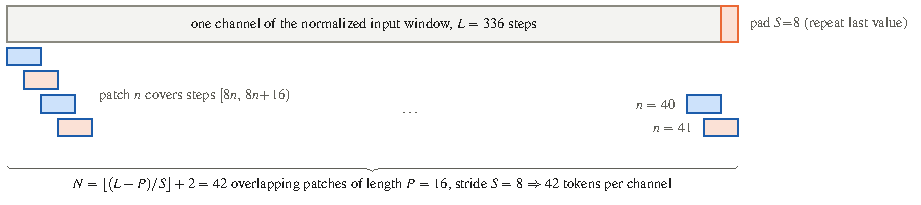
\includegraphics[width=\colfig]{fig_patching.pdf}
\caption{Patching of one channel. End padding with $S$ repeated values adds one patch, giving $N=42$ tokens for $L=336$, $P=16$, $S=8$.}
\label{fig:patching}
\end{figure}

\subsubsection{Embedding and encoder}
Each patch is mapped to a $D$-dimensional token by a shared linear layer, and a learnable position encoding $\mathbf{W}_{\mathrm{pos}}\in\R^{N\times D}$ is added:
\begin{equation}
\mathbf{e}_{c,n}=\mathbf{W}_P\,\mathbf{p}_{c,n}+\mathbf{b}_P,\qquad \mathbf{u}^{(0)}_{c,n}=\mathbf{e}_{c,n}+\mathbf{W}_{\mathrm{pos},n}.
\label{eq:embed}
\end{equation}
Channels are processed independently: the batch of $B$ windows becomes $B\cdot C$ sequences of $N$ tokens. Each of the three encoder layers applies multi-head self-attention with residual attention scores~\cite{realformer}, followed by a position-wise feed-forward network, each wrapped in a residual connection and BatchNorm~\cite{batchnorm}. For head $h$ in layer $l$,
\begin{equation}
\begin{gathered}
\mathbf{A}^{(l)}_h=\frac{\mathbf{Q}^{(l)}_h{\mathbf{K}^{(l)}_h}^{\top}}{\sqrt{d_k}}+\mathbf{A}^{(l-1)}_h,\\
\mathrm{head}^{(l)}_h=\mathrm{softmax}\big(\mathbf{A}^{(l)}_h\big)\,\mathbf{V}^{(l)}_h,
\end{gathered}
\label{eq:attn}
\end{equation}
where $\mathbf{A}^{(0)}_h=\mathbf{0}$ and $d_k=D/n_h$. The layer output is
\begin{align}
\mathbf{z}^{(l)}&=\mathrm{BN}\big(\mathbf{u}^{(l-1)}+\mathrm{Drop}(\mathrm{MHA}(\mathbf{u}^{(l-1)})\mathbf{W}_O)\big),\label{eq:layer1}\\
\mathbf{u}^{(l)}&=\mathrm{BN}\big(\mathbf{z}^{(l)}+\mathrm{Drop}(\mathbf{W}_2\,\mathrm{GELU}(\mathbf{W}_1\mathbf{z}^{(l)}))\big),\label{eq:layer2}
\end{align}
with GELU activation~\cite{gelu} and dropout~\cite{dropout}. We use $D=16$, $n_h=4$, a feed-forward width of 128 and dropout 0.3, the official settings for ETTh1.

\subsubsection{Head and de-normalization}
The $N$ output tokens of each channel are flattened into $\mathbf{h}_c\in\R^{ND}$ ($ND=672$), mapped to the horizon by a linear head, and the window statistics are restored:
\begin{equation}
\hat{\mathbf{y}}^{N}_c=\mathbf{W}_H\mathbf{h}_c+\mathbf{b}_H\in\R^{H},\qquad \hat{\mathbf{y}}_c=\sigma_c\,\hat{\mathbf{y}}^{N}_c+\mu_c.
\label{eq:head}
\end{equation}

\subsection{Patch Reliability Gate}
\label{sec:method-gate}

The gate is a small MLP that assigns every patch a weight $w_{c,n}\in(0,1)$ (Fig.~\ref{fig:gate}). Its input concatenates the 16 normalized values of the patch with seven summary features:
\begin{equation}
\begin{split}
\mathbf{g}_{c,n}=\mathrm{clip}_{[-10,10]}\Big(\big[&\mathbf{p}_{c,n};\ \bar{p}_{c,n};\ \varsigma_{c,n};\ j_{c,n};\\
&z_{c,n};\ a_{c,n};\ s^{\mu}_c;\ s^{\sigma}_c\big]\Big)\in\R^{23}.
\end{split}
\label{eq:gatein}
\end{equation}
Here $\bar{p}_{c,n}$ and $\varsigma_{c,n}$ are the mean and standard deviation of the patch, and $a_{c,n}=\max_k|p_{c,n,k}|$ is its largest absolute value. The jump feature compares a patch's mean with the average of its neighbours,
\begin{equation}
j_{c,n}=\Big|\bar{p}_{c,n}-\tfrac12\big(\bar{p}_{c,n-1}+\bar{p}_{c,n+1}\big)\Big|,
\label{eq:jump}
\end{equation}
with the first and last patch mean repeated at the borders. The zero share $z_{c,n}$ is the fraction of values in the corresponding patch of the \emph{un-normalized} (scaled) input that are exactly zero; it was designed to expose missing values, which the corruption model fills with the training mean, i.e., zero after scaling. The last two entries are the window-level shift features defined in~\eqref{eq:shift} below, broadcast to every patch of the channel. The gate is
\begin{equation}
w_{c,n}=\mathrm{sigmoid}\Big(\mathbf{v}_2^{\top}\,\mathrm{ReLU}\big(\mathbf{V}_1\mathbf{g}_{c,n}+\mathbf{c}_1\big)+c_2\Big),
\label{eq:gate}
\end{equation}
with $\mathbf{V}_1\in\R^{32\times23}$, $\mathbf{c}_1,\mathbf{v}_2\in\R^{32}$ and $c_2\in\R$. The weight rescales the patch embedding before the position encoding is added, replacing~\eqref{eq:embed} by
\begin{equation}
\mathbf{u}^{(0)}_{c,n}=w_{c,n}\big(\mathbf{W}_P\,\mathbf{p}_{c,n}+\mathbf{b}_P\big)+\mathbf{W}_{\mathrm{pos},n}.
\label{eq:gated}
\end{equation}
Applying the gate before the position encoding means that a fully distrusted patch still occupies its position in the sequence but carries no content. The output bias is initialized to $c_2=4$, so that $w\approx\mathrm{sigmoid}(4)\approx0.982$ at the start of training and the model initially behaves like PatchTST. The gate has $23\cdot32+32+32+1=801$ parameters. No supervision tells the gate which patches are corrupted; it is trained only through the forecasting loss. The code also supports an optional penalty $\lambda(1-\bar{w})$ that discourages uniformly low weights, but it was not used ($\lambda=0$) in any reported run.

\begin{figure}[!t]
\centering
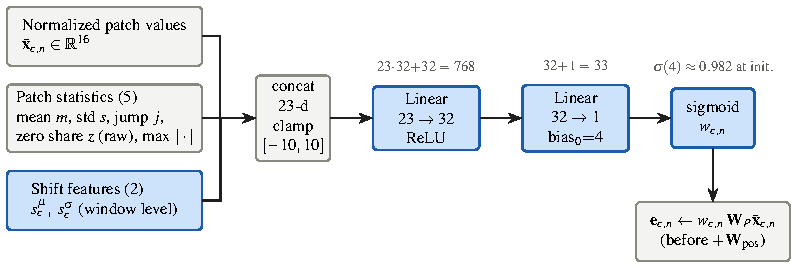
\includegraphics[width=\linewidth]{fig_gate.pdf}
\caption{Reliability gate. Each patch is scored from its 16 normalized values, five patch statistics and the two shift features of its channel. The score multiplies the patch embedding.}
\label{fig:gate}
\end{figure}

\subsection{Shift-Aware Head}
\label{sec:method-shift}

Instance normalization~\eqref{eq:revin} makes the encoder blind to where a window sits relative to the data the model was trained on: a window whose level has moved by two standard deviations looks the same after normalization as an ordinary one. The window statistics are added back at the output~\eqref{eq:head}, but only as an affine correction, so the shape of the forecast cannot depend on them. We compute two shift numbers per channel,
\begin{equation}
s^{\mu}_c=\frac{\mu_c-\bar{\mu}_c}{\bar{\sigma}_c},\qquad s^{\sigma}_c=\frac{\sigma_c}{\bar{\sigma}_c},
\label{eq:shift}
\end{equation}
and append them to the flattened encoder output before the head:
\begin{equation}
\hat{\mathbf{y}}^{N}_c=\mathbf{W}'_H\big[\mathbf{h}_c;\ s^{\mu}_c;\ s^{\sigma}_c\big]+\mathbf{b}_H,\qquad \mathbf{W}'_H\in\R^{H\times(ND+2)}.
\label{eq:shifthead}
\end{equation}
This adds $2H=192$ parameters. The idea is related to the de-stationary attention of Non-stationary Transformers~\cite{nstransformer}, which also reinjects removed statistics, but here they enter only the linear head. The same two numbers feed the gate.

\subsection{Corruption Model}
\label{sec:method-corrupt}

All corruptions act on scaled input windows, so a unit of one corresponds to one training standard deviation. Let $\mathbf{M}$ denote the mask of altered positions, $\odot$ the element-wise product and $\mathcal{B}(p)$ an independent Bernoulli draw per position.

\textit{Missing values (point):} $\mathbf{M}\sim\mathcal{B}(p)$ and $\tilde{\X}=(\mathbf{1}-\mathbf{M})\odot\X$, i.e., each dropped value is replaced by the training mean (zero).

\textit{Missing values (16-step stretch):} a stretch starts at each position with probability $p/16$ and zeroes the next 16 values of that channel, so the expected coverage is close to $p$ and a whole patch length can be lost at once.

\textit{Noise:} $\mathbf{M}\sim\mathcal{B}(p)$ and $\tilde{\X}=\X+\mathbf{M}\odot\bm{\epsilon}$ with $\epsilon_{i,c}\sim\mathcal{N}(0,1)$.

\textit{Anomaly (spike):} $\mathbf{M}\sim\mathcal{B}(p)$ and $\tilde{\X}=\X+\mathbf{M}\odot\mathbf{r}\odot\mathbf{a}$ with magnitudes $a_{i,c}\sim\mathcal{U}(3,5)$ and random signs $r_{i,c}\in\{-1,+1\}$.

\textit{Shift:} for each window and channel, $k$ segments of length $\lfloor L/10\rfloor=33$ with random start are transformed as
\begin{equation}
\tilde{x}_{i,c}=\alpha\,x_{i,c}+\beta,\qquad \alpha\sim\mathcal{U}(0.5,2),\quad \beta\sim\mathcal{U}(-2,2),
\label{eq:shiftcorr}
\end{equation}
with independent $(\alpha,\beta)$ per segment. Segments may overlap.

\textit{Mixed:} shift with $k=1$, then noise, spikes and point-wise missing values, each at $p=5\%$. Missing values are applied last so that dropped values stay exactly zero.

The severity levels are $p\in\{1,5,10,15\}\%$ of points for the first four types and $k\in\{1,3,5,10\}$ segments for shift. Fig.~\ref{fig:corr} shows each type on a real test window.

\begin{figure*}[!t]
\centering
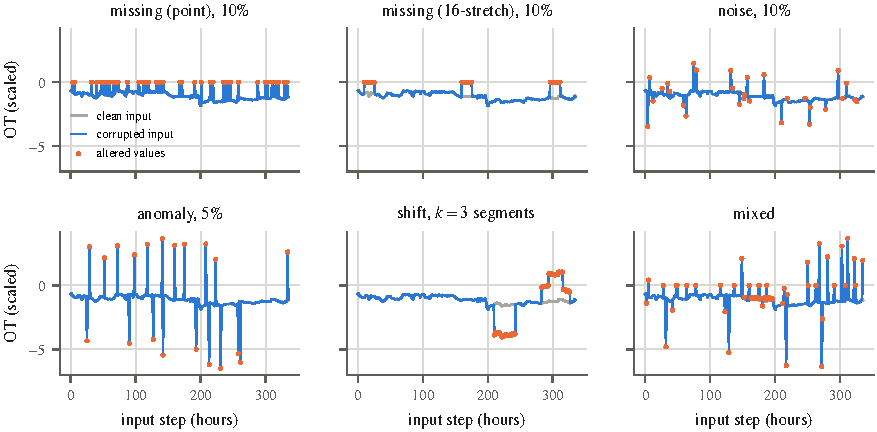
\includegraphics[width=\figwidth]{fig_corruptions.pdf}
\caption{The corruption types applied to one ETTh1 test input window (oil temperature channel, scaled units). Grey: clean input; blue: corrupted input; orange dots: altered values. The panels were drawn with a NumPy port of the project's corruption functions using the same distributions and parameters.}
\label{fig:corr}
\end{figure*}

\subsection{Corruption-Aware Training}
\label{sec:method-cat}

During training each window in a mini-batch is corrupted independently with probability $0.5$ (Fig.~\ref{fig:cat}). For a corrupted window the type is drawn uniformly from \{missing, noise, anomaly, shift\} and the level index uniformly from the four levels; a missing-value corruption is point-wise or stretch-wise with equal probability. The mixed setting is never used for training. The loss~\eqref{eq:mse} is always computed against the clean future, so the network learns to forecast the true continuation from damaged evidence. Because corruption is drawn afresh at every step, the model sees a different damaged copy of each window in every epoch.

\begin{figure}[!t]
\centering
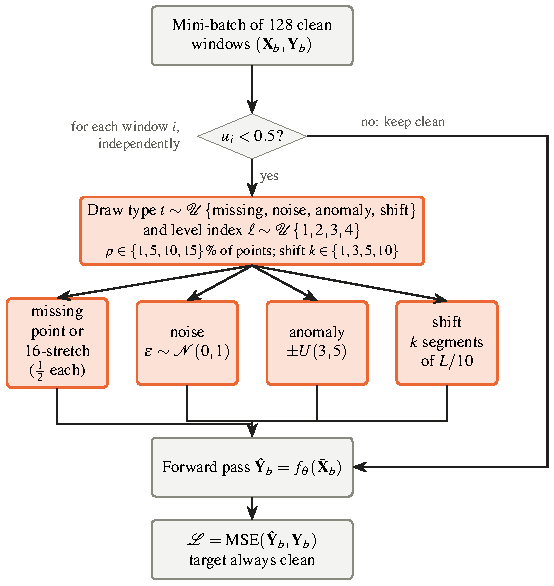
\includegraphics[width=\colfig]{fig_cat.pdf}
\caption{Corruption-aware training. Each window of a mini-batch is corrupted with probability 0.5 using a randomly chosen type and severity. The forecasting loss always uses the clean target.}
\label{fig:cat}
\end{figure}

\subsection{Optimization and Model Selection}
\label{sec:method-opt}

All variants use Adam~\cite{adam} with an initial learning rate $\eta_0=10^{-4}$, batch size 128 and the step decay of the official code (its ``type3'' schedule),
\begin{equation}
\eta_e=\eta_0\cdot0.9^{\max(0,\,e-4)},\qquad e=1,2,\dots
\label{eq:lr}
\end{equation}
Training runs for at most 20 epochs. After each epoch we evaluate the validation MSE on clean windows and on a fixed mixed-corruption copy of the validation set, and keep the checkpoint that minimizes
\begin{equation}
J=\tfrac12\big(\mathrm{MSE}_{\mathrm{val}}^{\mathrm{clean}}+\mathrm{MSE}_{\mathrm{val}}^{\mathrm{mixed}}\big).
\label{eq:select}
\end{equation}
Early stopping uses the same criterion with patience 5. We also keep the checkpoint with the lowest clean validation MSE, which is used only to report the clean reproduction of PatchTST. Algorithm~\ref{alg:train} summarizes the procedure.

\begin{algorithm}[!t]
\caption{Training and selection of one RA-PatchTST variant}
\label{alg:train}
\small
\begin{algorithmic}[1]
\Require training windows $\mathcal{D}_{\mathrm{tr}}$, validation windows $\mathcal{D}_{\mathrm{va}}$, variant flags (gate, shift head, CAT), seed
\State $\tilde{\mathcal{D}}_{\mathrm{va}}\gets$ mixed corruption of $\mathcal{D}_{\mathrm{va}}$ with seed 777
\State initialize $\theta$; gate output bias $c_2\gets4$; $J^\star\gets\infty$; $bad\gets0$
\For{$e=1$ \textbf{to} $20$}
  \State $\eta\gets10^{-4}\cdot0.9^{\max(0,e-4)}$
  \For{each mini-batch $(\X_b,\Y_b)$ of 128 windows, shuffled, last partial batch dropped}
    \If{CAT} \State $\X_b\gets$ corrupt each window with probability 0.5 (random type and level) \EndIf
    \State $\hat{\Y}_b\gets f_\theta(\X_b)$ \Comment{Eqs.~\eqref{eq:revin}--\eqref{eq:shifthead}}
    \State $\theta\gets\mathrm{Adam}\big(\theta,\nabla_\theta\,\mathrm{MSE}(\hat{\Y}_b,\Y_b),\eta\big)$
  \EndFor
  \State $J\gets\frac12\big(\mathrm{MSE}(f_\theta,\mathcal{D}_{\mathrm{va}})+\mathrm{MSE}(f_\theta,\tilde{\mathcal{D}}_{\mathrm{va}})\big)$
  \If{$J<J^\star$} \State $J^\star\gets J$;\ $\theta^\star\gets\theta$;\ $bad\gets0$ \Else \State $bad\gets bad+1$ \EndIf
  \If{$bad\ge5$} \textbf{break} \EndIf
\EndFor
\State \Return $\theta^\star$
\end{algorithmic}
\end{algorithm}

\subsection{Model Variants}
\label{sec:method-variants}

The ablation adds one component at a time (Table~\ref{tab:variants}). A0 is the PatchTST baseline. A1 adds corruption-aware training only, so it isolates the effect of the training data. A2 and A3 add the shift-aware head and the gate respectively on top of A1, and A4 is the full RA-PatchTST. Two further variants are defined in the code, A5 (A4 without corruption-aware training) and A6 (A4 with a gate that does not see the shift features), but they were not run and no result is reported for them.

\begin{table}[!t]
\centering
\caption{Model Variants of the Ablation}
\label{tab:variants}
\footnotesize
\colfit{%
\begin{tabular}{@{}lcccrl@{}}
\toprule
Variant & CAT & Shift head & Gate & Params & Status \\
\midrule
A0 PatchTST & -- & -- & -- & 81,728 & run, 2 seeds \\
A1 & \checkmark & -- & -- & 81,728 & run, 2 seeds \\
A2 & \checkmark & \checkmark & -- & 81,920 & run, 2 seeds \\
A3 & \checkmark & -- & \checkmark & 82,529 & run, 2 seeds \\
A4 RA-PatchTST & \checkmark & \checkmark & \checkmark & 82,721 & run, 2 seeds \\
A5 & -- & \checkmark & \checkmark & 82,721 & defined, not run \\
A6 & \checkmark & \checkmark & \checkmark$^{\dagger}$ & 82,657 & defined, not run \\
\bottomrule
\multicolumn{6}{@{}p{0.95\linewidth}@{}}{\scriptsize CAT: corruption-aware training. $^{\dagger}$Gate without the two shift features (21 inputs instead of 23).}
\end{tabular}}
\end{table}

\subsection{Complexity}
\label{sec:method-complexity}

For a batch of $B$ windows, self-attention costs $O(B\,C\,N^2 D)$ per layer and the feed-forward network $O(B\,C\,N\,D\,d_{ff})$. The gate adds $O(B\,C\,N\cdot(23\cdot32+32))$ operations, roughly the cost of one extra feed-forward layer of width 32 on the patch tokens, and the shift head adds $O(B\,C\,H)$. Neither changes the asymptotic cost. The parameter count of the backbone breaks down as follows: patch embedding 272, position encoding 672, three encoder layers of 5,392 each (attention projections 1,088, two BatchNorms 64, feed-forward 4,240) and the head 64,608, for 81,728 in total. The head dominates, and the gate and shift head together add 993 parameters (1.2\%).

\section{System Architecture}
\label{sec:arch}

The system has two parts: a Python research pipeline that prepares the data, corrupts inputs, trains and evaluates the variants and produces the reports, and a self-contained browser application that runs the trained baseline and RA-PatchTST side by side. Fig.~\ref{fig:pipeline} shows how data move through the pipeline.

\begin{figure*}[!t]
\centering
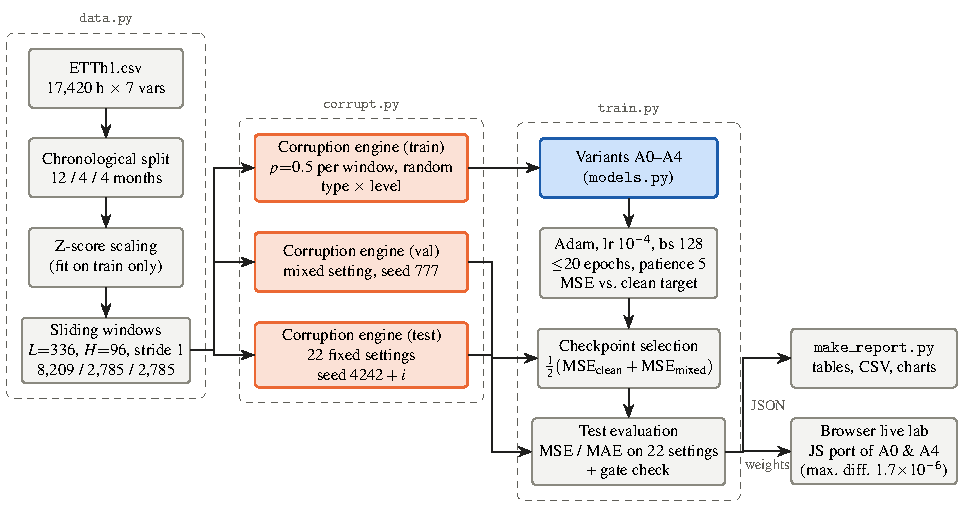
\includegraphics[width=0.92\textwidth]{fig_pipeline.pdf}
\caption{End-to-end pipeline. The same corruption engine produces random corruptions during training, one fixed mixed corruption of the validation set for model selection, and 22 fixed, seeded corruptions of the test set. Results are written as JSON files from which every table and chart is generated; the weights of A0 and A4 are exported to the browser application.}
\label{fig:pipeline}
\end{figure*}

\subsection{Module Design}

The code base consists of five Python modules with narrow interfaces (Table~\ref{tab:modules}). The data module returns tensors only and knows nothing about corruption. The corruption engine is a set of pure functions that take a scaled batch and a seeded random generator and return the corrupted batch together with the mask of altered positions; the same functions serve training, validation and testing, so the corruption seen in evaluation is guaranteed to be the one described in Section~\ref{sec:method-corrupt}. The model module defines a single class whose constructor flags switch the gate and the shift head on or off, and a table that maps each variant name to its flags. The training module owns optimization, selection, evaluation and the gate check, and writes one JSON file per (variant, seed). The report module reads only those JSON files.

\begin{table*}[!t]
\centering
\caption{Software Modules, Responsibilities and Interfaces}
\label{tab:modules}
\footnotesize
\renewcommand{\arraystretch}{1.15}
\begin{tabular}{@{}p{0.14\textwidth}p{0.42\textwidth}p{0.38\textwidth}@{}}
\toprule
Module & Responsibility & Input $\rightarrow$ output \\
\midrule
\texttt{data.py} & Chronological split, train-only scaling, sliding windows, training statistics & CSV file $\rightarrow$ train/val/test tensors, $\bar{\mu}_c,\bar{\sigma}_c$ \\
\texttt{corrupt.py} & Five corruption types, 22 test settings, training-time corruption, patch masks & window batch, seed $\rightarrow$ corrupted batch, mask \\
\texttt{models.py} & PatchTST backbone, reliability gate, shift head; variants A0 to A6 & window batch $\rightarrow$ forecast (and gate weights) \\
\texttt{train.py} & Training loop, checkpoint selection, resumable per-epoch checkpoints, test sweep, gate check & variant, seed $\rightarrow$ result JSON \\
\texttt{make\_report.py} & Aggregation over seeds, tables and charts & result JSON files $\rightarrow$ Markdown, CSV, PNG \\
Live lab (HTML) & JavaScript forward pass of A0 and A4 with embedded weights and test windows & user edits $\rightarrow$ two forecasts, errors, gate weights \\
\bottomrule
\end{tabular}
\end{table*}

\subsection{Tensor Flow Through the Model}

Table~\ref{tab:shapes} traces the shape of the data through one forward pass for a batch of $B$ windows. Channel independence is implemented by folding the channel axis into the batch axis before the encoder and unfolding it before the head; the gate and shift features are computed per channel before folding.

\begin{table}[!t]
\centering
\caption{Tensor Shapes in One Forward Pass}
\label{tab:shapes}
\footnotesize
\colfit{%
\begin{tabular}{@{}ll@{}}
\toprule
Stage & Shape \\
\midrule
Input window $\X$ & $(B,\ 336,\ 7)$ \\
Window statistics $\mu,\sigma$; shift numbers $s^{\mu},s^{\sigma}$ & $(B,\ 7)$ each \\
Patches $\mathbf{p}$ & $(B,\ 7,\ 42,\ 16)$ \\
Gate input $\mathbf{g}$ / gate weights $w$ & $(B,\ 7,\ 42,\ 23)$ / $(B,\ 7,\ 42)$ \\
Embeddings $\mathbf{u}^{(0)}$ (channels folded) & $(7B,\ 42,\ 16)$ \\
Encoder output & $(7B,\ 42,\ 16)$ \\
Head input $[\mathbf{h}_c;s^{\mu}_c;s^{\sigma}_c]$ & $(B,\ 7,\ 674)$ \\
Forecast $\hat{\Y}$ & $(B,\ 96,\ 7)$ \\
\bottomrule
\end{tabular}}
\end{table}

\subsection{Evaluation Subsystem}

Evaluation is deterministic by design. Test setting $i$ ($i=0,\dots,21$) is generated once from the clean test windows with generator seed $4242+i$, and the validation mixed set with seed 777, so all variants and seeds are scored on identical corrupted inputs. For the gated variants the evaluation also reads the gate weights for seven representative settings and splits them by a patch-level mask: a patch counts as corrupted if any of its 16 values was altered, computed by padding and unfolding the position mask exactly as the input is patched.

\subsection{Interactive Live Laboratory}

The live laboratory is a single HTML file that needs no server or network connection. It contains a JavaScript port of the forward pass of A0 and A4 (seed 2021), their trained weights, and a fixed set of 24 ETTh1 test windows. A user picks a window and a channel, applies damage through presets (missing stretches, noise, spikes, level and scale shifts, mixed) or by dragging individual readings, and sees the true future, both forecasts, the damaged input and the trust that the A4 gate gives each patch. A benchmark button runs both models on all $24\times7=168$ sample series under the current damage settings. A dashboard tab shows the experimental results of Section~\ref{sec:results} and states their limitations. When the page was built, the JavaScript forward pass was compared with PyTorch on sample windows and differed by at most $1.7\times10^{-6}$.

\section{Implementation}
\label{sec:impl}

\subsection{Environment}

The system is written in Python~3 with PyTorch~\cite{pytorch}, NumPy and pandas, and matplotlib for the charts. All experiments ran on a cloud CPU container with two virtual cores (Intel Xeon class, 2.1~GHz). Training used two worker processes with one thread each, running the (variant, seed) jobs in a fixed priority order; the script skips jobs whose result file already exists and saves a checkpoint after every epoch, so an interrupted schedule resumes where it stopped. No GPU was used, and a laptop CPU is sufficient to reproduce every run at roughly 40~s per epoch.

\subsection{Hyperparameters}

Table~\ref{tab:hparams} lists every setting. The backbone values are those of the official PatchTST script for ETTh1. No hyperparameter search was carried out for any variant; all variants share the same settings and training budget, so differences between them are attributable to the components being ablated and to seed variation.

\begin{table}[!t]
\centering
\caption{Hyperparameters (Identical for All Variants)}
\label{tab:hparams}
\footnotesize
\colfit{%
\begin{tabular}{@{}ll@{}}
\toprule
Setting & Value \\
\midrule
Look-back $L$ / horizon $H$ & 336 / 96 \\
Patch length $P$ / stride $S$ / patches $N$ & 16 / 8 / 42 \\
Encoder layers / heads / $D$ / FFN width & 3 / 4 / 16 / 128 \\
Dropout & 0.3 \\
Gate hidden width / output bias init. & 32 / $+4$ \\
Gate input clamp & $[-10,10]$ \\
Optimizer / initial learning rate & Adam / $10^{-4}$ \\
Learning-rate decay & $\times0.9$ per epoch after epoch 4 \\
Batch size & 128 (last partial batch dropped) \\
Max.\ epochs / early-stopping patience & 20 / 5 \\
Corruption probability in training & 0.5 per window \\
Training seeds & 2021, 2022 \\
Validation / test corruption seeds & 777 / $4242+i$ \\
Gate penalty $\lambda$ & 0 (not used) \\
\bottomrule
\end{tabular}}
\end{table}

\subsection{Faithfulness to the Official PatchTST}

The backbone was re-implemented from the official code~\cite{patchtst_code} rather than imported, so that the gate and shift head could be inserted at the exact points shown in Fig.~\ref{fig:arch}. It reproduces instance normalization without affine parameters, end padding, patch length 16 with stride 8, the learnable position encoding initialized uniformly in $[-0.02,0.02]$, post-norm encoder layers with BatchNorm, residual attention scores and GELU, and the flatten-linear head. Three small deviations were made, all documented with the code:
\begin{enumerate}
\item dropout is implemented with a uniform random mask ($\mathbf{x}\odot\mathbb{1}[\mathbf{u}\ge p]/(1-p)$, $\mathbf{u}\sim\mathcal{U}(0,1)$), which is mathematically the same inverted dropout but about twice as fast on the CPU;
\item the gate input is clamped to $[-10,10]$ to keep spikes from saturating the gate MLP;
\item the checkpoint used for corrupted-data results is chosen by the combined criterion~\eqref{eq:select} instead of clean validation loss alone, and the clean-validation checkpoint is kept separately for the reproduction check.
\end{enumerate}
The training budget is also smaller than the official one (20 epochs instead of up to 100), which is discussed with the results.

\subsection{Verification}

Before the experiments, the pipeline was checked with the tests in Table~\ref{tab:tests}. They confirm the split sizes, that scaling uses training statistics only, that corruption is deterministic for a given seed and touches only masked positions, that parameter counts match the design, that the untrained gate starts near one, that saved weights reproduce the stored results, and that the browser port agrees with PyTorch.

\begin{table*}[!t]
\centering
\caption{Verification Tests and Their Outcomes}
\label{tab:tests}
\footnotesize
\renewcommand{\arraystretch}{1.12}
\begin{tabular}{@{}lp{0.19\textwidth}p{0.22\textwidth}p{0.18\textwidth}p{0.24\textwidth}l@{}}
\toprule
ID & Purpose & Input & Expected & Observed & Result \\
\midrule
T1 & Window counts & ETTh1, $L=336$, $H=96$ & 8,209 / 2,785 / 2,785 & 8,209 / 2,785 / 2,785 & Pass \\
T2 & Train-only scaling & Training split & Mean 0, std 1 per variable & 0.0 and 1.0 for all 7 variables & Pass \\
T3 & Deterministic corruption & Mixed corruption, seed 4242 twice, then 4243 & Same seed identical; different seed differs & Identical; differs & Pass \\
T4 & Only masked values change & Missing, noise, spike, shift on 128 windows & Unmasked values unchanged & Unchanged for all four; 9.9\% altered at the 10\% level & Pass \\
T5 & Parameter counts & A0, A4, gate & 81,728 / 82,721 / 801 & 81,728 / 82,721 / 801 & Pass \\
T6 & Untrained gate near 1 & A4, untrained, 32 windows & $\approx0.98$ & 0.984 & Pass \\
T7 & Saved weights reproduce results & A0 and A4, seed 2021, clean and mixed test MSE & Match result files & 0.3785/0.4491 (A0), 0.3815/0.4276 (A4) & Pass \\
T8 & Browser port matches PyTorch & Sample windows & Max.\ difference $<10^{-5}$ & $1.7\times10^{-6}$ & Pass \\
T9 & Baseline reproduces paper & ETTh1, $H=96$ & Within 2\% of 0.375 & 0.379 ($+1.1\%$) & Pass \\
\bottomrule
\end{tabular}
\end{table*}

\subsection{Reproducibility}

All randomness is seeded. The training seed fixes model initialization, batch order and, through a separate generator offset by 1000, the training-time corruption. Corrupted evaluation sets use their own fixed seeds. The public ETTh1 file is used unchanged. Every number in Section~\ref{sec:results} is computed by script from the per-run JSON files, which also store the per-epoch training history; the tables and figures of this paper were regenerated from those files.

\section{Experimental Setup}
\label{sec:exp}

\subsection{Dataset}

ETTh1 is the hourly subset of the Electricity Transformer Temperature dataset introduced with Informer~\cite{informer} and distributed through the ETDataset repository~\cite{ettdata} and the Time-Series-Library~\cite{tslib_code}. The file covers 1 July 2016 to 26 June 2018 (17,420 hourly records) from one power transformer in China. It has seven variables: six load features (high, middle and low useful and useless load: HUFL, HULL, MUFL, MULL, LUFL, LULL) and the oil temperature OT. We found no missing values, no duplicate timestamps and no gaps in the hourly spacing. The load features contain negative values and large excursions (HUFL ranges from $-22.7$ to $23.6$), which we keep because they are part of the recorded signal. The data contain no personal information.

Following the standard protocol, the first 12 months form the training set, the next four months the validation set and the following four months the test set; the remaining 3,020 hours are not used. Table~\ref{tab:split} gives the periods and window counts, and Fig.~\ref{fig:dataset} shows two of the variables with the split. The test period falls in winter. Its mean oil temperature is 4.85 against 17.13 in the training year, and the standard deviation of HUFL is 7.66 against 5.81, so even the clean test set is shifted relative to training. Because windows are cut with stride 1, neighbouring samples overlap and are not independent.

\begin{table}[!t]
\centering
\caption{Chronological Split of ETTh1}
\label{tab:split}
\footnotesize
\colfit{%
\begin{tabular}{@{}llr@{}}
\toprule
Split & Period (hourly records) & Windows ($L{=}336$, $H{=}96$) \\
\midrule
Train & 2016-07-01 to 2017-06-25 (8,640) & 8,209 \\
Validation & 2017-06-26 to 2017-10-23 (2,880) & 2,785 \\
Test & 2017-10-24 to 2018-02-20 (2,880) & 2,785 \\
\bottomrule
\end{tabular}}
\end{table}

\begin{figure*}[!t]
\centering
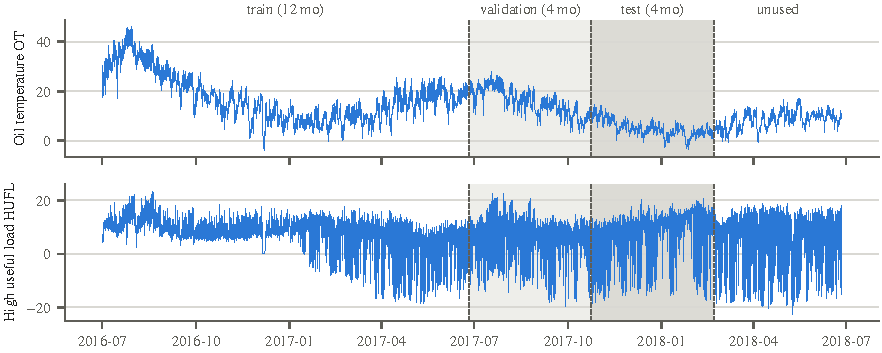
\includegraphics[width=\figwidth]{fig_dataset.pdf}
\caption{Two ETTh1 variables over the full recording with the chronological split. The shaded regions are the validation and test periods; the last 3,020 hours are not used.}
\label{fig:dataset}
\end{figure*}

\subsection{Test Conditions}

Each model is evaluated on 22 versions of the 2,785 test windows (Table~\ref{tab:settings}): the clean inputs, four severity levels for each of the five corruption families, and the mixed setting. Only the input windows are corrupted; the target is the clean future in every case. The mixed setting combines all four training families but at a fixed combination never seen during training.

\begin{table}[!t]
\centering
\caption{The 22 Test Conditions}
\label{tab:settings}
\footnotesize
\renewcommand{\arraystretch}{1.12}
\colfit{%
\begin{tabular}{@{}p{0.28\linewidth}p{0.36\linewidth}p{0.24\linewidth}@{}}
\toprule
Family & Parameters & Levels \\
\midrule
Clean & none & 1 \\
Missing (point) & fraction $p$ of values set to 0 & $p\in\{1,5,10,15\}\%$ \\
Missing (16-stretch) & stretches of 16 zeros, coverage $\approx p$ & $p\in\{1,5,10,15\}\%$ \\
Noise & $+\mathcal{N}(0,1)$ on fraction $p$ & $p\in\{1,5,10,15\}\%$ \\
Anomaly (spike) & $\pm\,\mathcal{U}(3,5)$ on fraction $p$ & $p\in\{1,5,10,15\}\%$ \\
Shift & $k$ segments of 33 steps, $\alpha\!\sim\!\mathcal{U}(0.5,2)$, $\beta\!\sim\!\mathcal{U}(-2,2)$ & $k\in\{1,3,5,10\}$ \\
Mixed & shift $k{=}1$ + noise, spike, missing at 5\% each & 1 \\
\bottomrule
\end{tabular}}
\end{table}

\subsection{Metrics}

We report the mean squared error and mean absolute error on the scaled data,
\begin{equation}
\begin{gathered}
\mathrm{MSE}=\frac{1}{|\mathcal{T}|HC}\sum_{\mathcal{T}}\sum_{i=1}^{H}\sum_{c=1}^{C}(\hat{y}_{i,c}-y_{i,c})^2,\\
\mathrm{MAE}=\frac{1}{|\mathcal{T}|HC}\sum_{\mathcal{T}}\sum_{i=1}^{H}\sum_{c=1}^{C}|\hat{y}_{i,c}-y_{i,c}|,
\end{gathered}
\label{eq:metrics}
\end{equation}
where $\mathcal{T}$ is the set of test windows; lower is better for both. Scaled units make the numbers comparable with published ETTh1 results. Results are aggregated by family (mean over the four levels) and as the mean over all 21 corrupted conditions. Relative change against a reference variant is $\Delta=100\,(\mathrm{MSE}_{v}/\mathrm{MSE}_{\mathrm{ref}}-1)\%$, computed from seed-averaged values, so negative values mean improvement. Gate behaviour is measured as the mean gate weight over corrupted and over clean patches.

\subsection{Statistical Treatment}

Each variant was trained with two seeds (2021 and 2022). We report means with the sample standard deviation over the two seeds, the per-seed values for the headline numbers, and a paired comparison of each variant with A1 in each seed. Two seeds and overlapping test windows do not support formal significance tests or confidence intervals, so we do not report any; the standard deviations should be read as indicating the spread between two runs, nothing more.

\subsection{Baselines}

The baseline is our PatchTST re-implementation (A0). No other published method was re-run under this protocol, so the paper makes no claim about RA-PatchTST relative to DLinear, iTransformer, SEER, TFPS, APT or any other model.

\section{Results and Discussion}
\label{sec:results}

All results are on the ETTh1 test split (2,785 windows, horizon 96, scaled units) and are means over two seeds unless stated otherwise. Table~\ref{tab:headline} gives the headline comparison between the baseline and the full model with the per-seed values; Tables~\ref{tab:groups-mse} to~\ref{tab:delta-a1} break the results down by corruption family and variant, and Appendix~\ref{app:full} lists every condition.

\begin{table}[!t]
\centering
\caption{Headline Results: PatchTST (A0) Versus RA-PatchTST (A4)}
\label{tab:headline}
\footnotesize
\colfit{%
\begin{tabular}{@{}llccl@{}}
\toprule
Model & Test condition & MSE & MAE & Per-seed MSE \\
\midrule
\tabin{tab_headline}
\bottomrule
\end{tabular}}
\end{table}

\subsection{Clean-Data Reproduction (O1)}

Table~\ref{tab:repro} reports the clean test error of each variant with the checkpoint chosen on clean validation loss, which is how PatchTST is usually evaluated. The baseline A0 reaches MSE 0.3791 and MAE 0.4008, against 0.375 and 0.399 published for PatchTST/42~\cite{patchtst}, a gap of 1.1\% in MSE and 0.5\% in MAE, which meets the 2\% target. The remaining gap is plausibly due to the shorter training budget: seed 2021 of A0 reached its best validation score in the last allowed epoch (Table~\ref{tab:cost}), so it had not finished improving. In every run the two checkpoint rules happened to select the same epoch, so the clean numbers in Tables~\ref{tab:headline} and~\ref{tab:repro} coincide.

\begin{table}[!t]
\centering
\caption{Clean Test Error With the Clean-Validation Checkpoint, Against the Published PatchTST/42 Result (MSE 0.375, MAE 0.399)}
\label{tab:repro}
\footnotesize
\colfit{%
\begin{tabular}{@{}lcccc@{}}
\toprule
Variant & MSE & MAE & $\Delta$MSE vs.\ paper & $\Delta$MAE vs.\ paper \\
\midrule
\tabin{tab_repro}
\bottomrule
\end{tabular}}
\end{table}

\subsection{How Much Does Corruption Hurt PatchTST? (RQ1)}

The baseline degrades very unevenly across corruption families (first column of Table~\ref{tab:groups-mse}, Fig.~\ref{fig:groups}). Point-wise missing values, 16-step stretches and noise raise its MSE by only 0.005 to 0.013 on average, and even at 15\% the worst of them costs 7\% (missing stretches, 0.406). Spikes raise the mean MSE to 0.458 ($+20.9\%$) and segment-level shift to 0.520 ($+37.1\%$); at ten shifted segments the MSE reaches 0.712, 88\% above the clean value. Averaged over all 21 corrupted conditions the baseline loses 13.3\%.

Instance normalization explains most of this pattern. A zero in a scaled series is the training mean, which instance normalization turns into a moderate value, and Gaussian noise of one standard deviation on a few percent of the points barely changes the window statistics. A spike of 3 to 5 standard deviations, on the other hand, inflates $\sigma_c$ in~\eqref{eq:revin}, which compresses every other value of the window after normalization and then stretches the forecast when the statistics are restored. A shifted segment moves both $\mu_c$ and $\sigma_c$ and changes the local shape that the patches encode. In both cases the damage spreads, through the window statistics, to every patch of the window.

\begin{table*}[!t]
\centering
\caption{Test MSE by Corruption Family (Mean $\pm$ Standard Deviation Over Two Seeds; Best in Bold)}
\label{tab:groups-mse}
\footnotesize
\begin{tabular}{@{}lccccc@{}}
\toprule
Test condition & A0 PatchTST & A1 +CAT & A2 +CAT+shift head & A3 +CAT+gate & A4 RA-PatchTST \\
\midrule
\tabin{tab_groups_mse}
\bottomrule
\end{tabular}
\end{table*}

\begin{table*}[!t]
\centering
\caption{Test MAE by Corruption Family (Mean $\pm$ Standard Deviation Over Two Seeds; Best in Bold)}
\label{tab:groups-mae}
\footnotesize
\begin{tabular}{@{}lccccc@{}}
\toprule
Test condition & A0 PatchTST & A1 +CAT & A2 +CAT+shift head & A3 +CAT+gate & A4 RA-PatchTST \\
\midrule
\tabin{tab_groups_mae}
\bottomrule
\end{tabular}
\end{table*}

\begin{figure*}[!t]
\centering
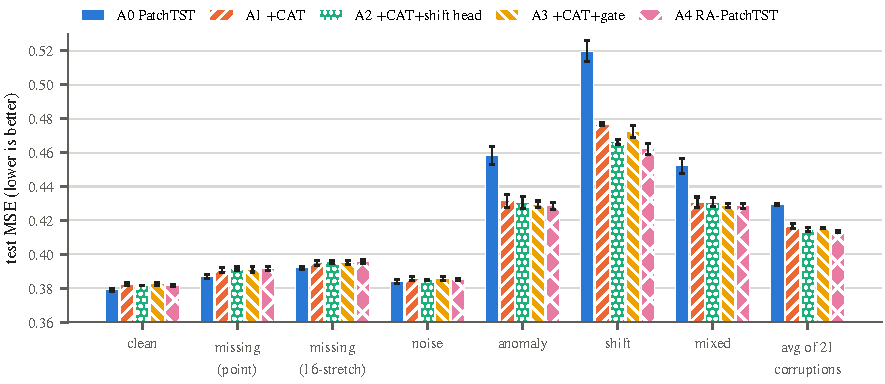
\includegraphics[width=\figwidth]{fig_mse_groups.pdf}
\caption{Test MSE by corruption family for the five variants (mean over two seeds; error bars show the standard deviation between seeds). Note that the vertical axis starts at 0.36.}
\label{fig:groups}
\end{figure*}

\subsection{Effect of RA-PatchTST (RQ2, H1)}

The full model lowers the average MSE over the 21 corrupted conditions from 0.429 to 0.413, a reduction of 3.7\% (Table~\ref{tab:delta-a0}). The reduction is 11.0\% under shift, 6.5\% under spikes and 5.2\% in the mixed setting, and the same ordering holds for MAE (Table~\ref{tab:groups-mae}). The price is a small loss elsewhere: $+0.7\%$ on clean inputs, $+1.3\%$ under point-wise missing values, $+0.9\%$ under missing stretches and $+0.2\%$ under noise. A4 beats A0 in 10 of the 21 corrupted conditions: all four spike levels, all four shift levels, the mixed setting and noise at 15\%. It is worse in the remaining eleven, all of them missing-value or low-level noise conditions where the baseline was already close to its clean error.

The improvement grows with severity (Fig.~\ref{fig:severity}). At one shifted segment A4 is 1.6\% better than A0, at ten segments 20.1\% better (0.569 against 0.712). For spikes the gain rises from 0.6\% at 1\% of points to 11.0\% at 15\%. Fig.~\ref{fig:heatmap} shows the same effect as degradation relative to each model's own clean error: A0 loses 88\% at the worst condition, A4 49\%, and averaged over the 21 conditions A0 loses 13.3\% and A4 8.3\%. For missing values the curves of the three models run nearly parallel, with A0 slightly below.

Against the success criteria of Section~\ref{sec:problem}, A4 lowers the average corrupted MSE in both seeds (0.4132 and 0.4137 against 0.4289 and 0.4298), raises clean MSE by 0.7\% (below the 2\% limit) and adds 1.2\% parameters (below 5\%). H1 is therefore supported on this dataset, with the qualification that the gain is concentrated in two corruption families.

\begin{table}[!t]
\centering
\caption{Change in Test MSE Relative to A0 (Negative Means Better)}
\label{tab:delta-a0}
\footnotesize
\colfit{%
\begin{tabular}{@{}lcccc@{}}
\toprule
Test condition & A1 & A2 & A3 & A4 \\
\midrule
\tabin{tab_delta_a0}
\bottomrule
\end{tabular}}
\end{table}

\begin{figure*}[!t]
\centering
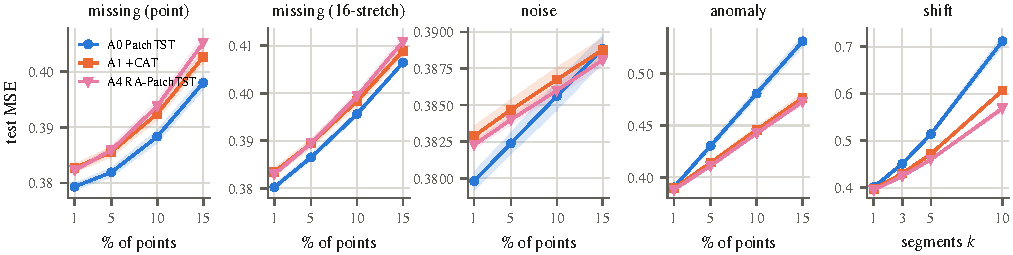
\includegraphics[width=\figwidth]{fig_severity.pdf}
\caption{Test MSE against corruption severity for A0, A1 and A4. Lines are seed means; the shaded bands span the two seeds. Note the different vertical scales.}
\label{fig:severity}
\end{figure*}

\begin{figure*}[!t]
\centering
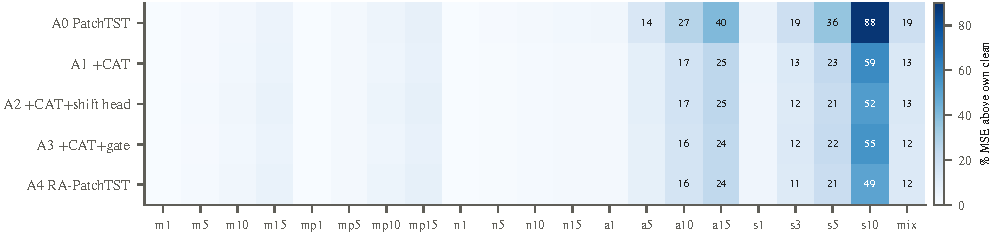
\includegraphics[width=\figwidth]{fig_heatmap.pdf}
\caption{Degradation of each variant relative to its own clean error, $100(\mathrm{MSE}_{\mathrm{cond}}/\mathrm{MSE}_{\mathrm{clean}}-1)$, for the 21 corrupted conditions (m: missing point, mp: missing 16-stretch, n: noise, a: anomaly, s: shift; numbers give the percentage level or the number of shifted segments). Cells of 10\% or more are labelled.}
\label{fig:heatmap}
\end{figure*}

\subsection{Ablation: Where Does the Gain Come From?}

Training on corrupted inputs alone (A1) already gives $-3.0\%$ of the $-3.7\%$ average reduction, that is, about four fifths of the total (Table~\ref{tab:delta-a0}, Fig.~\ref{fig:ablation}). Measured against A1 (Table~\ref{tab:delta-a1}), the shift-aware head (A2) adds $-0.5\%$ on average and $-2.2\%$ under shift, the gate (A3) adds $-0.3\%$ and $-0.9\%$, and the two together (A4) add $-0.8\%$ and $-3.0\%$. The effects of the two components add up almost exactly, which suggests that they address different parts of the problem: the head corrects the level and scale of the forecast, while the gate changes which patches the encoder relies on.

The shift-aware head is the more useful of the two architectural additions, as the analysis of RQ1 would predict: under shift the model needs the window level and scale that instance normalization removes, and the head gives them back. A2 and A4 also reach lower validation errors than A1 and A3 on both the clean and the mixed validation sets (Fig.~\ref{fig:learning}), which points to a benefit that is not limited to the test period.

\begin{table}[!t]
\centering
\caption{Change in Test MSE Relative to A1 (Corruption-Aware Training Only)}
\label{tab:delta-a1}
\footnotesize
\colfit{%
\begin{tabular}{@{}lccc@{}}
\toprule
Test condition & A2 & A3 & A4 \\
\midrule
\tabin{tab_delta_a1}
\bottomrule
\end{tabular}}
\end{table}

\begin{figure}[!t]
\centering
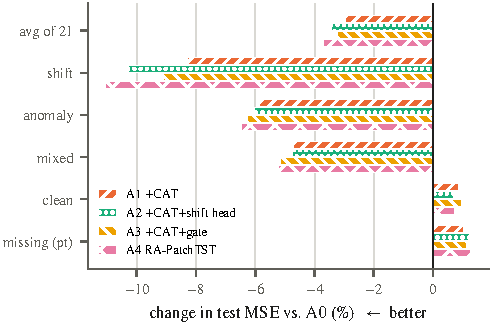
\includegraphics[width=\colfig]{fig_ablation.pdf}
\caption{Change in test MSE relative to A0 for each variant and selected condition groups. Bars to the left of zero are improvements.}
\label{fig:ablation}
\end{figure}

\subsection{Are the Differences Consistent Across Seeds?}

Table~\ref{tab:paired} compares each variant with A1 seed by seed on the average of the 21 corrupted conditions. All three variants improve on A1 in both seeds, and A4 does so by 0.0025 and 0.0039. These differences are small, of the same order as the gap between the two seeds of A1 (0.0020), and with two seeds no significance can be claimed. The comparison with A0 is on firmer ground: the difference between A0 and A4 (0.016) is about 18 times the seed spread of A0 (0.0009) and 32 times that of A4 (0.0005).

\begin{table}[!t]
\centering
\caption{Paired Per-Seed Comparison With A1 on the Average of the 21 Corrupted Conditions}
\label{tab:paired}
\footnotesize
\colfit{%
\begin{tabular}{@{}lcccl@{}}
\toprule
Variant & Seeds & Mean $\Delta$MSE & Seeds better & Per-seed $\Delta$MSE \\
\midrule
\tabin{tab_paired}
\bottomrule
\end{tabular}}
\end{table}

\subsection{Does the Gate Detect Corrupted Patches? (H2)}

Table~\ref{tab:gate} and Fig.~\ref{fig:gate-w} compare the mean gate weight on corrupted and clean patches for seven representative conditions. The gate does react to spikes: in A4 a patch containing a spike receives 0.939 on average, against 0.964 for clean patches in the same windows, and in A3 the gap is wider (0.926 against 0.963). Smaller gaps appear for shift ($-0.017$) and noise ($-0.007$). For missing values, which the zero-share feature was meant to expose, the gate hardly separates damaged from clean patches (a gap of 0.002 to 0.004).

All weights lie between 0.92 and 0.97, so the gate never comes close to switching a patch off; it behaves more like a mild global rescaling with a small extra discount on suspicious patches than like a filter. The gap is also largest for A3, where the gate is the only architectural addition, which suggests that in A4 the shift head takes over part of the work the gate would otherwise do. H2 is supported only weakly, and only for spikes. We therefore do not attribute the robustness of RA-PatchTST mainly to the gate.

\begin{table*}[!t]
\centering
\caption{Mean Gate Weight on Corrupted and Clean Patches (1.0: Fully Trusted). A Patch Counts as Corrupted if Any of Its 16 Values Was Altered}
\label{tab:gate}
\footnotesize
\begin{tabular}{@{}lccccccc@{}}
\toprule
 & & \multicolumn{3}{c}{A3 (+CAT+gate)} & \multicolumn{3}{c}{A4 (RA-PatchTST)} \\
\cmidrule(lr){3-5}\cmidrule(l){6-8}
Condition & Share corrupted & Corrupted & Clean & Gap & Corrupted & Clean & Gap \\
\midrule
\tabin{tab_gate}
\bottomrule
\end{tabular}
\end{table*}

\begin{figure*}[!t]
\centering
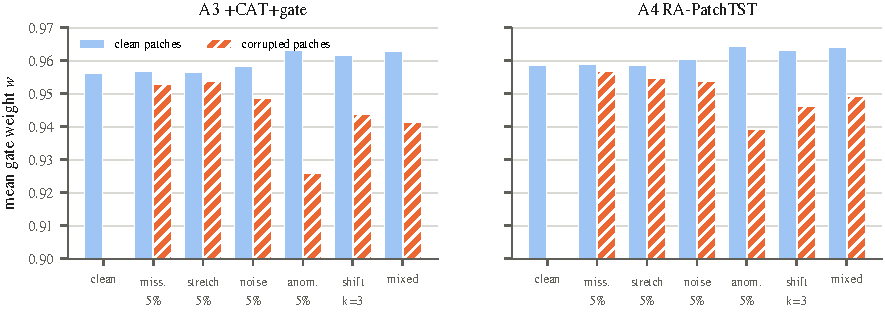
\includegraphics[width=\figwidth]{fig_gate_weights.pdf}
\caption{Mean gate weight on clean and corrupted patches for A3 and A4 (mean over two seeds). The vertical axis spans 0.90 to 0.97: every weight is close to one, and a clear gap appears only for spikes.}
\label{fig:gate-w}
\end{figure*}

\subsection{Training Dynamics}

Fig.~\ref{fig:learning} shows the validation curves. All runs used the full 20 epochs, and the selected checkpoints come from epochs 17 to 20 (Table~\ref{tab:cost}), so none of the models had clearly converged; the official schedule allows up to 100 epochs. On clean validation data A0 ends with the lowest error, as expected for the only model trained on clean data alone. On the mixed validation set the order reverses: at the selected epochs A4 reaches 0.729 to 0.734 and A0 0.761 to 0.765. In every variant the validation MSE is much higher than the test MSE (about 0.68 against 0.38 on clean data), so the two periods differ in difficulty and selection on the validation period transfers to the test period only approximately. Corruption-aware variants also end with higher training loss (0.383 to 0.388 against 0.357 to 0.358 for A0), because half of their training windows are corrupted.

\begin{figure*}[!t]
\centering
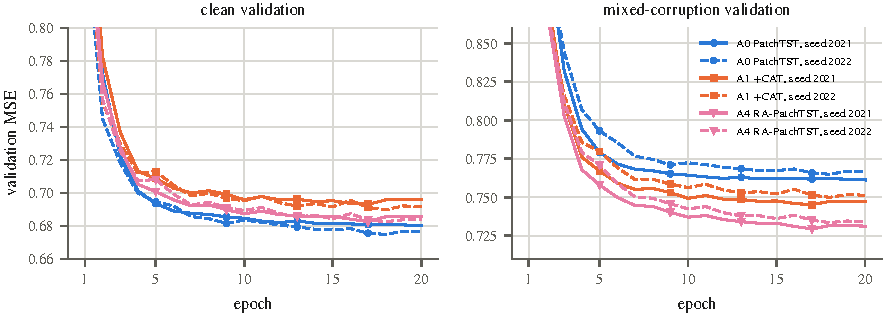
\includegraphics[width=\figwidth]{fig_learning.pdf}
\caption{Validation MSE per epoch for A0, A1 and A4 on clean (left) and mixed-corruption (right) validation windows. Solid lines: seed 2021; dashed lines: seed 2022.}
\label{fig:learning}
\end{figure*}

\subsection{Computational Cost}

Table~\ref{tab:cost} lists the cost of each variant. RA-PatchTST has 993 more parameters than PatchTST (1.2\%), of which 801 are in the gate and 192 in the head. Training time per epoch on one CPU thread rises from 37.0~s to 41.2~s ($+11\%$); 2.0~s of the increase comes from generating corruptions (A1 against A0), 2.0~s from the gate (A3 against A1) and under 1~s from the shift head (A2 against A1). Inference on the 2,785 test windows takes 4.2 to 5.5~s for all variants, and the differences between variants lie within the timing noise of a shared CPU.

\begin{table}[!t]
\centering
\caption{Model Size and Cost (Training Time on One CPU Thread; Inference Over 2,785 Test Windows)}
\label{tab:cost}
\footnotesize
\colfit{%
\begin{tabular}{@{}lrrrccc@{}}
\toprule
Variant & Params & $\Delta$ & Gate & s/epoch & Infer.\ (s) & Sel.\ epoch \\
\midrule
\tabin{tab_cost}
\bottomrule
\multicolumn{7}{@{}l@{}}{\scriptsize Sel.\ epoch: epoch of the selected checkpoint for seeds 2021/2022 (max.\ 20).}
\end{tabular}}
\end{table}

\subsection{Interactive Demonstration}

On the fixed set of 24 test windows $\times$ 7 channels in the live laboratory, with the mixed damage preset, the browser models (seed 2021) give MSE 0.433 for PatchTST and 0.426 for RA-PatchTST ($-1.5\%$), and RA-PatchTST is better on 112 of the 168 series. This is a small demonstration set and not part of the evaluation, but it agrees in direction with the test results.

\subsection{Discussion}

\subsubsection{Interpretation}
The baseline reproduces PatchTST closely and loses accuracy mainly under spikes and shift, in line with the concerns raised about window-local normalization~\cite{fan,apt,revinrole} and patch-level shift~\cite{tfps}. RA-PatchTST reduces these losses, and most of the reduction is due to the training data: a PatchTST that simply sees corrupted windows during training (A1) recovers about 80\% of the gain. The architectural additions help, mostly under shift, and the more effective of them is the simplest one, two numbers appended to the head. The gate learns to discount spikes a little but does not detect missing values.

\subsubsection{Why missing values get slightly worse}
All corruption-aware variants are 0.7 to 1.3\% worse than A0 under missing values and on clean data. Two causes are plausible. First, capacity and training signal are shared: the model spends part of both on spikes and shift, the most damaging families, at a small cost on the mild ones. Second, the zero-filling corruption is easy for the baseline to absorb (a zero is the training mean), so there is little to gain and some precision to lose. The weak response of the gate to missing values may also have a simple cause: the zero-share feature in~\eqref{eq:gatein} is one of 23 inputs, and nothing in the loss rewards the gate for using it.

\subsubsection{Practical significance}
The extra cost is small: 993 parameters, about 11\% more training time and no measurable inference overhead. For data that are mostly clean and complete, RA-PatchTST brings almost no benefit and a slight loss of accuracy. For sensors that are prone to spikes, recalibration jumps or regime changes, the reduction of up to 20\% at high shift severity is a meaningful gain. The model is a research prototype and has not been validated in operation.

\subsubsection{Limitations and threats to validity}
\label{sec:limitations}
The evidence is narrow. Only one dataset (ETTh1), one horizon (96) and one look-back (336) were tested, with two seeds and a 20-epoch budget, and no hyperparameters were tuned. No other published method was re-run, so nothing is claimed relative to SEER~\cite{seer}, TFPS~\cite{tfps}, APT~\cite{apt} or DLinear~\cite{dlinear}. The test corruptions come from the same families that were used in training (only their combination in the mixed setting is new), so the results show robustness to known corruption types, not to unseen ones. The corruptions are synthetic and may differ from real sensor faults. Test windows overlap, so naive confidence intervals would be too narrow. The differences between A2, A3, A4 and A1 are of the same order as the seed variation. Variants A5 and A6 and the gate penalty were not run, so we cannot say how the gate behaves without corruption-aware training or without the shift features. Error analysis by channel or by horizon step was not carried out.

\section{Future Scope}
\label{sec:future}

The limitations above point directly to the next steps, which we order from the most to the least immediate.

\subsubsection{Complete the ablation and strengthen the statistics}
Run at least five seeds per variant, complete A5 (no corruption-aware training) and A6 (gate without shift features), and test the gate penalty $\lambda$. Replace the two-seed standard deviations with confidence intervals from a moving-block bootstrap over test windows~\cite{kunsch}, which respects the overlap between neighbouring windows.

\subsubsection{Broaden the benchmark}
Repeat the protocol on ETTm1, Weather and Electricity and at horizons 192, 336 and 720, with the full training budget of the official code. Re-run DLinear~\cite{dlinear}, iTransformer~\cite{itransformer}, SEER~\cite{seer}, TFPS~\cite{tfps} and APT~\cite{apt} under the same corruption protocol so that the comparison no longer rests on a single baseline.

\subsubsection{Test generalization to unseen damage}
Hold corruption families out of training (for example, train without shift and test with it), add corruption types not modelled here such as stuck-at values, drift ramps and quantization, and evaluate on series with real logged sensor faults rather than synthetic ones.

\subsubsection{Improve the gate}
Give the gate an explicit missing-value mask where the data pipeline can supply one, add a weak auxiliary loss on synthetic corruptions that teaches it where damage is (the corruption engine already produces the mask), and let it act on the attention scores as well as the embeddings. The current result, a gate that stays near one, suggests that the forecasting loss alone gives it too little reason to discriminate.

\subsubsection{Extend the shift signal}
The two shift numbers proved the most useful addition. Richer global descriptors, such as frequency-domain statistics in the spirit of FAN~\cite{fan} or timestamp prototypes as in APT~\cite{apt}, could be passed to the head in the same cheap way, and the effect on clean accuracy should be checked across datasets.

\subsubsection{Towards deployment}
Couple the gate weights with a calibrated uncertainty estimate so that low trust in the input can be reported to an operator, and measure latency on embedded hardware typical of substation monitoring.

\section{Conclusion}
\label{sec:conclusion}

PatchTST gives every input patch the same trust and normalizes away the level and scale of each window, which makes it sensitive to spikes and to shifts in the input. We proposed RA-PatchTST, which adds a patch reliability gate, two shift features for the forecasting head and corruption-aware training, at a cost of 993 parameters, and evaluated it on ETTh1 against a PatchTST re-implementation that reproduces the published clean error to within 1.1\%. Across 21 corrupted test conditions the mean MSE fell from 0.429 to 0.413 ($-3.7\%$), with reductions of 11.0\% under shift, 6.5\% under spikes and 5.2\% under mixed damage, and of 20.1\% at the most severe shift; the clean error rose by 0.7\%.

The ablation qualifies these numbers. Training on corrupted inputs provides about four fifths of the gain. The shift-aware head adds most of the remainder and the gate a little more, and the two effects are additive. The gate discounts spiky patches but does not identify missing values, and its weights stay close to one. The study covers one dataset, one horizon and two seeds, with synthetic corruptions from the training families, so the evidence is preliminary. Within those limits, the results suggest that for patch-based forecasters a large part of the robustness to corrupted inputs can be bought cheaply, through the training data and a global view of shift, and that learning to distrust individual patches needs a stronger signal than the forecasting loss provides.


\section*{Acknowledgment}
The authors thank the Department of Computer Science and Engineering, Ramaiah Institute of Technology, for computing access and guidance. The ETTh1 dataset was released by Zhou \textit{et al.}~\cite{informer} through the ETDataset repository~\cite{ettdata}. The PatchTST re-implementation follows the official code of Nie \textit{et al.}~\cite{patchtst_code}, and the data protocol follows the Time-Series-Library~\cite{tslib_code}.

\bibliographystyle{IEEEtran}
\bibliography{refs}

\appendices
\section{Results for All 22 Test Conditions}
\label{app:full}

Table~\ref{tab:full} gives the test MSE of every variant for every test condition (mean over seeds 2021 and 2022), the MAE of A0 and A4, and the relative change in MSE of A4 against A0. The per-seed values of every run are stored in the result files of the project.

\begin{table*}[!t]
\centering
\caption{Test MSE of All Variants and MAE of A0 and A4 for Every Test Condition (Mean of Two Seeds; Lowest MSE in Bold)}
\label{tab:full}
\footnotesize
\begin{tabular}{@{}lccccccccc@{}}
\toprule
 & \multicolumn{5}{c}{MSE} & \multicolumn{2}{c}{MAE} & \\
\cmidrule(lr){2-6}\cmidrule(lr){7-8}
Condition & A0 & A1 & A2 & A3 & A4 & A0 & A4 & $\Delta$MSE A4 vs.\ A0 \\
\midrule
\tabin{tab_full}
\bottomrule
\end{tabular}
\end{table*}

\section{Data Dictionary}
\label{app:data}

\begin{table}[!h]
\centering
\caption{ETTh1 Variables (Original Units Are Not Stated in the Dataset Documentation)}
\label{tab:dict}
\footnotesize
\colfit{%
\begin{tabular}{@{}llrrrr@{}}
\toprule
Variable & Description & Mean & Std & Min & Max \\
\midrule
HUFL & High useful load & 7.38 & 7.07 & $-22.71$ & 23.64 \\
HULL & High useless load & 2.24 & 2.04 & $-4.76$ & 10.11 \\
MUFL & Middle useful load & 4.30 & 6.83 & $-25.09$ & 17.34 \\
MULL & Middle useless load & 0.88 & 1.81 & $-5.93$ & 7.75 \\
LUFL & Low useful load & 3.07 & 1.16 & $-1.19$ & 8.50 \\
LULL & Low useless load & 0.86 & 0.60 & $-1.37$ & 3.05 \\
OT & Oil temperature (target of interest) & 13.32 & 8.57 & $-4.08$ & 46.01 \\
\bottomrule
\multicolumn{6}{@{}l@{}}{\scriptsize Statistics over all 17,420 records. The \texttt{date} column (hourly timestamps) is dropped before modelling.}
\end{tabular}}
\end{table}

\section{Reproducing the Experiments}
\label{app:repro}

The experiments are reproduced with the commands below, run from the project folder with Python~3, PyTorch, NumPy, pandas and matplotlib installed.

\begin{footnotesize}
\begin{verbatim}
python data.py data_raw/ETTh1.csv
python train.py --variants A0 A1 A2 A3 A4 \
  --seeds 2021 2022 --epochs 20 --patience 5
python make_report.py
\end{verbatim}
\end{footnotesize}

\noindent The first command checks the split shapes, the second trains and evaluates all runs, and the third writes the summary tables and chart.

\noindent \texttt{run\_all.sh} contains the exact two-worker schedule that was used. The figures and tables of this paper are regenerated from the stored result files by \texttt{make\_figures.py} and \texttt{make\_tables.py} in the manuscript repository.


\end{document}
